\documentclass[twoside]{book}

% Packages required by doxygen
\usepackage{fixltx2e}
\usepackage{calc}
\usepackage{doxygen}
\usepackage[export]{adjustbox} % also loads graphicx
\usepackage{graphicx}
\usepackage[utf8]{inputenc}
\usepackage{makeidx}
\usepackage{multicol}
\usepackage{multirow}
\PassOptionsToPackage{warn}{textcomp}
\usepackage{textcomp}
\usepackage[nointegrals]{wasysym}
\usepackage[table]{xcolor}

% Font selection
\usepackage[T1]{fontenc}
\usepackage[scaled=.90]{helvet}
\usepackage{courier}
\usepackage{amssymb}
\usepackage{sectsty}
\renewcommand{\familydefault}{\sfdefault}
\allsectionsfont{%
  \fontseries{bc}\selectfont%
  \color{darkgray}%
}
\renewcommand{\DoxyLabelFont}{%
  \fontseries{bc}\selectfont%
  \color{darkgray}%
}
\newcommand{\+}{\discretionary{\mbox{\scriptsize$\hookleftarrow$}}{}{}}

% Page & text layout
\usepackage{geometry}
\geometry{%
  a4paper,%
  top=2.5cm,%
  bottom=2.5cm,%
  left=2.5cm,%
  right=2.5cm%
}
\tolerance=750
\hfuzz=15pt
\hbadness=750
\setlength{\emergencystretch}{15pt}
\setlength{\parindent}{0cm}
\setlength{\parskip}{3ex plus 2ex minus 2ex}
\makeatletter
\renewcommand{\paragraph}{%
  \@startsection{paragraph}{4}{0ex}{-1.0ex}{1.0ex}{%
    \normalfont\normalsize\bfseries\SS@parafont%
  }%
}
\renewcommand{\subparagraph}{%
  \@startsection{subparagraph}{5}{0ex}{-1.0ex}{1.0ex}{%
    \normalfont\normalsize\bfseries\SS@subparafont%
  }%
}
\makeatother

% Headers & footers
\usepackage{fancyhdr}
\pagestyle{fancyplain}
\fancyhead[LE]{\fancyplain{}{\bfseries\thepage}}
\fancyhead[CE]{\fancyplain{}{}}
\fancyhead[RE]{\fancyplain{}{\bfseries\leftmark}}
\fancyhead[LO]{\fancyplain{}{\bfseries\rightmark}}
\fancyhead[CO]{\fancyplain{}{}}
\fancyhead[RO]{\fancyplain{}{\bfseries\thepage}}
\fancyfoot[LE]{\fancyplain{}{}}
\fancyfoot[CE]{\fancyplain{}{}}
\fancyfoot[RE]{\fancyplain{}{\bfseries\scriptsize Generated by Doxygen }}
\fancyfoot[LO]{\fancyplain{}{\bfseries\scriptsize Generated by Doxygen }}
\fancyfoot[CO]{\fancyplain{}{}}
\fancyfoot[RO]{\fancyplain{}{}}
\renewcommand{\footrulewidth}{0.4pt}
\renewcommand{\chaptermark}[1]{%
  \markboth{#1}{}%
}
\renewcommand{\sectionmark}[1]{%
  \markright{\thesection\ #1}%
}

% Indices & bibliography
\usepackage{natbib}
\usepackage[titles]{tocloft}
\setcounter{tocdepth}{3}
\setcounter{secnumdepth}{5}
\makeindex

% Hyperlinks (required, but should be loaded last)
\usepackage{ifpdf}
\ifpdf
  \usepackage[pdftex,pagebackref=true]{hyperref}
\else
  \usepackage[ps2pdf,pagebackref=true]{hyperref}
\fi
\hypersetup{%
  colorlinks=true,%
  linkcolor=blue,%
  citecolor=blue,%
  unicode%
}

% Custom commands
\newcommand{\clearemptydoublepage}{%
  \newpage{\pagestyle{empty}\cleardoublepage}%
}

\usepackage{caption}
\captionsetup{labelsep=space,justification=centering,font={bf},singlelinecheck=off,skip=4pt,position=top}

%===== C O N T E N T S =====

\begin{document}

% Titlepage & ToC
\hypersetup{pageanchor=false,
             bookmarksnumbered=true,
             pdfencoding=unicode
            }
\pagenumbering{alph}
\begin{titlepage}
\vspace*{7cm}
\begin{center}%
{\Large Extremum Search \\[1ex]\large 1.\+0 }\\
\vspace*{1cm}
{\large Generated by Doxygen 1.8.13}\\
\end{center}
\end{titlepage}
\clearemptydoublepage
\pagenumbering{roman}
\tableofcontents
\clearemptydoublepage
\pagenumbering{arabic}
\hypersetup{pageanchor=true}

%--- Begin generated contents ---
\chapter{Hierarchical Index}
\section{Class Hierarchy}
This inheritance list is sorted roughly, but not completely, alphabetically\+:\begin{DoxyCompactList}
\item \contentsline{section}{Area}{\pageref{class_area}}{}
\begin{DoxyCompactList}
\item \contentsline{section}{N\+Cube}{\pageref{class_n_cube}}{}
\item \contentsline{section}{Range}{\pageref{class_range}}{}
\end{DoxyCompactList}
\item \contentsline{section}{Function}{\pageref{class_function}}{}
\begin{DoxyCompactList}
\item \contentsline{section}{Smooth\+Function}{\pageref{class_smooth_function}}{}
\item \contentsline{section}{Test\+Func01}{\pageref{class_test_func01}}{}
\item \contentsline{section}{Test\+Func02}{\pageref{class_test_func02}}{}
\item \contentsline{section}{Test\+Func03}{\pageref{class_test_func03}}{}
\item \contentsline{section}{Test\+Func04}{\pageref{class_test_func04}}{}
\item \contentsline{section}{Test\+Func05}{\pageref{class_test_func05}}{}
\end{DoxyCompactList}
\item \contentsline{section}{Optimization\+Method}{\pageref{class_optimization_method}}{}
\begin{DoxyCompactList}
\item \contentsline{section}{Nelder\+Mead}{\pageref{class_nelder_mead}}{}
\item \contentsline{section}{Random\+Search}{\pageref{class_random_search}}{}
\end{DoxyCompactList}
\item \contentsline{section}{Opt\+Result}{\pageref{struct_opt_result}}{}
\item \contentsline{section}{Simplex}{\pageref{class_simplex}}{}
\item \contentsline{section}{Terminal\+Condition}{\pageref{class_terminal_condition}}{}
\begin{DoxyCompactList}
\item \contentsline{section}{Count\+Condition}{\pageref{class_count_condition}}{}
\begin{DoxyCompactList}
\item \contentsline{section}{Condition\+Improvement}{\pageref{class_condition_improvement}}{}
\item \contentsline{section}{Condition\+Iter}{\pageref{class_condition_iter}}{}
\end{DoxyCompactList}
\item \contentsline{section}{Eps\+Condition}{\pageref{class_eps_condition}}{}
\begin{DoxyCompactList}
\item \contentsline{section}{Condition\+F\+Diff}{\pageref{class_condition_f_diff}}{}
\item \contentsline{section}{Condition\+Grad}{\pageref{class_condition_grad}}{}
\item \contentsline{section}{Condition\+X\+Diff}{\pageref{class_condition_x_diff}}{}
\end{DoxyCompactList}
\end{DoxyCompactList}
\item \contentsline{section}{v\+Point}{\pageref{classv_point}}{}
\end{DoxyCompactList}

\chapter{Class Index}
\section{Class List}
Here are the classes, structs, unions and interfaces with brief descriptions\+:\begin{DoxyCompactList}
\item\contentsline{section}{\hyperlink{class_area}{Area} }{\pageref{class_area}}{}
\item\contentsline{section}{\hyperlink{class_condition_f_diff}{Condition\+F\+Diff} }{\pageref{class_condition_f_diff}}{}
\item\contentsline{section}{\hyperlink{class_condition_grad}{Condition\+Grad} }{\pageref{class_condition_grad}}{}
\item\contentsline{section}{\hyperlink{class_condition_improvement}{Condition\+Improvement} }{\pageref{class_condition_improvement}}{}
\item\contentsline{section}{\hyperlink{class_condition_iter}{Condition\+Iter} }{\pageref{class_condition_iter}}{}
\item\contentsline{section}{\hyperlink{class_condition_x_diff}{Condition\+X\+Diff} }{\pageref{class_condition_x_diff}}{}
\item\contentsline{section}{\hyperlink{class_count_condition}{Count\+Condition} }{\pageref{class_count_condition}}{}
\item\contentsline{section}{\hyperlink{class_eps_condition}{Eps\+Condition} }{\pageref{class_eps_condition}}{}
\item\contentsline{section}{\hyperlink{class_function}{Function} }{\pageref{class_function}}{}
\item\contentsline{section}{\hyperlink{class_n_cube}{N\+Cube} }{\pageref{class_n_cube}}{}
\item\contentsline{section}{\hyperlink{class_nelder_mead}{Nelder\+Mead} }{\pageref{class_nelder_mead}}{}
\item\contentsline{section}{\hyperlink{class_optimization_method}{Optimization\+Method} }{\pageref{class_optimization_method}}{}
\item\contentsline{section}{\hyperlink{struct_opt_result}{Opt\+Result} }{\pageref{struct_opt_result}}{}
\item\contentsline{section}{\hyperlink{class_random_search}{Random\+Search} }{\pageref{class_random_search}}{}
\item\contentsline{section}{\hyperlink{class_range}{Range} }{\pageref{class_range}}{}
\item\contentsline{section}{\hyperlink{class_simplex}{Simplex} }{\pageref{class_simplex}}{}
\item\contentsline{section}{\hyperlink{class_smooth_function}{Smooth\+Function} }{\pageref{class_smooth_function}}{}
\item\contentsline{section}{\hyperlink{class_terminal_condition}{Terminal\+Condition} }{\pageref{class_terminal_condition}}{}
\item\contentsline{section}{\hyperlink{class_test_func01}{Test\+Func01} }{\pageref{class_test_func01}}{}
\item\contentsline{section}{\hyperlink{class_test_func02}{Test\+Func02} }{\pageref{class_test_func02}}{}
\item\contentsline{section}{\hyperlink{class_test_func03}{Test\+Func03} }{\pageref{class_test_func03}}{}
\item\contentsline{section}{\hyperlink{class_test_func04}{Test\+Func04} }{\pageref{class_test_func04}}{}
\item\contentsline{section}{\hyperlink{class_test_func05}{Test\+Func05} }{\pageref{class_test_func05}}{}
\item\contentsline{section}{\hyperlink{classv_point}{v\+Point} }{\pageref{classv_point}}{}
\end{DoxyCompactList}

\chapter{File Index}
\section{File List}
Here is a list of all documented files with brief descriptions\+:\begin{DoxyCompactList}
\item\contentsline{section}{{\bfseries area.\+h} }{\pageref{area_8h}}{}
\item\contentsline{section}{{\bfseries commands.\+h} }{\pageref{commands_8h}}{}
\item\contentsline{section}{{\bfseries condition\+\_\+f\+\_\+difference.\+h} }{\pageref{condition__f__difference_8h}}{}
\item\contentsline{section}{{\bfseries condition\+\_\+grad.\+h} }{\pageref{condition__grad_8h}}{}
\item\contentsline{section}{{\bfseries condition\+\_\+improvement.\+h} }{\pageref{condition__improvement_8h}}{}
\item\contentsline{section}{{\bfseries condition\+\_\+iter.\+h} }{\pageref{condition__iter_8h}}{}
\item\contentsline{section}{{\bfseries condition\+\_\+x\+\_\+difference.\+h} }{\pageref{condition__x__difference_8h}}{}
\item\contentsline{section}{{\bfseries count\+\_\+condition.\+h} }{\pageref{count__condition_8h}}{}
\item\contentsline{section}{{\bfseries eps\+\_\+condition.\+h} }{\pageref{eps__condition_8h}}{}
\item\contentsline{section}{\hyperlink{function_8h}{function.\+h} }{\pageref{function_8h}}{}
\item\contentsline{section}{{\bfseries ncube.\+h} }{\pageref{ncube_8h}}{}
\item\contentsline{section}{{\bfseries nelder\+\_\+mead.\+h} }{\pageref{nelder__mead_8h}}{}
\item\contentsline{section}{{\bfseries optimization\+\_\+method.\+h} }{\pageref{optimization__method_8h}}{}
\item\contentsline{section}{{\bfseries random\+\_\+search.\+h} }{\pageref{random__search_8h}}{}
\item\contentsline{section}{{\bfseries random\+\_\+seed.\+h} }{\pageref{random__seed_8h}}{}
\item\contentsline{section}{{\bfseries range.\+h} }{\pageref{range_8h}}{}
\item\contentsline{section}{{\bfseries Simplex.\+h} }{\pageref{_simplex_8h}}{}
\item\contentsline{section}{{\bfseries smooth\+\_\+function.\+h} }{\pageref{smooth__function_8h}}{}
\item\contentsline{section}{{\bfseries terminal\+\_\+condition.\+h} }{\pageref{terminal__condition_8h}}{}
\item\contentsline{section}{{\bfseries test\+\_\+func\+\_\+01.\+h} }{\pageref{test__func__01_8h}}{}
\item\contentsline{section}{{\bfseries test\+\_\+func\+\_\+02.\+h} }{\pageref{test__func__02_8h}}{}
\item\contentsline{section}{{\bfseries test\+\_\+func\+\_\+03.\+h} }{\pageref{test__func__03_8h}}{}
\item\contentsline{section}{{\bfseries test\+\_\+func\+\_\+04.\+h} }{\pageref{test__func__04_8h}}{}
\item\contentsline{section}{{\bfseries test\+\_\+func\+\_\+05.\+h} }{\pageref{test__func__05_8h}}{}
\item\contentsline{section}{{\bfseries variables.\+h} }{\pageref{variables_8h}}{}
\item\contentsline{section}{{\bfseries vpoint.\+h} }{\pageref{vpoint_8h}}{}
\end{DoxyCompactList}

\chapter{Class Documentation}
\hypertarget{class_area}{}\section{Area Class Reference}
\label{class_area}\index{Area@{Area}}


{\ttfamily \#include $<$area.\+h$>$}

Inheritance diagram for Area\+:\begin{figure}[H]
\begin{center}
\leavevmode
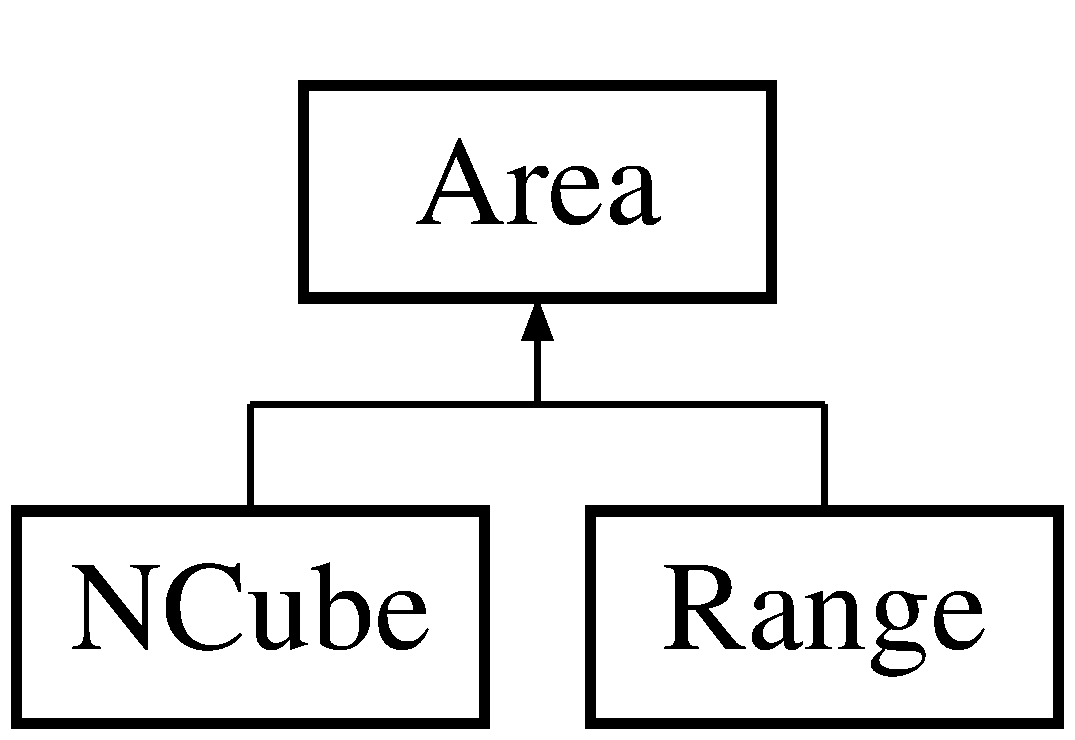
\includegraphics[height=2.000000cm]{class_area}
\end{center}
\end{figure}
\subsection*{Public Member Functions}
\begin{DoxyCompactItemize}
\item 
\hyperlink{class_area_acb26df340d249e1704501d55cacbc93e}{Area} (int \+\_\+dim)
\item 
virtual \hyperlink{class_area_a5ed5a9705b2715f347b764894c5015f0}{$\sim$\+Area} ()
\item 
virtual bool \hyperlink{class_area_a08775973fcf205fb91654b25a08f6bea}{In} (const \hyperlink{classv_point}{v\+Point} \&X) const =0
\item 
virtual \hyperlink{classv_point}{v\+Point} \hyperlink{class_area_a8a921495c0cca4095c8386f7b48ef086}{Random\+Point} () const =0
\item 
virtual std\+::shared\+\_\+ptr$<$ \hyperlink{class_area}{Area} $>$ \hyperlink{class_area_a8f28e6be12d6b1bf7217f51307ab937e}{Sub\+Area} (const \hyperlink{classv_point}{v\+Point} \&X, double epsilon) const =0
\item 
int \hyperlink{class_area_a4a7d5f99dd276ecc047fe75f448432ec}{Get\+Dim} () const
\begin{DoxyCompactList}\small\item\em returns the dimension of the area \end{DoxyCompactList}\item 
virtual void \hyperlink{class_area_abc427001b3685b08cd836badffedfbbe}{Info} () const =0
\end{DoxyCompactItemize}
\subsection*{Protected Attributes}
\begin{DoxyCompactItemize}
\item 
\mbox{\Hypertarget{class_area_ad1b73c86b972c92515c26f9f6a78afab}\label{class_area_ad1b73c86b972c92515c26f9f6a78afab}} 
int \hyperlink{class_area_ad1b73c86b972c92515c26f9f6a78afab}{dim}
\begin{DoxyCompactList}\small\item\em the dimension of the area \end{DoxyCompactList}\end{DoxyCompactItemize}
\subsection*{Friends}
\begin{DoxyCompactItemize}
\item 
std\+::ostream \& \hyperlink{class_area_ada6f29b8de500da1ce8e36efb839d484}{operator$<$$<$} (std\+::ostream \&out, std\+::shared\+\_\+ptr$<$ \hyperlink{class_area}{Area} $>$ A)
\end{DoxyCompactItemize}


\subsection{Detailed Description}
\hypertarget{function_8h_DESCRIPTION}{}\subsection{D\+E\+S\+C\+R\+I\+P\+T\+I\+ON}\label{function_8h_DESCRIPTION}
The \hyperlink{class_area}{Area} class represents a multidimensional subset of real vector points 

\subsection{Constructor \& Destructor Documentation}
\mbox{\Hypertarget{class_area_acb26df340d249e1704501d55cacbc93e}\label{class_area_acb26df340d249e1704501d55cacbc93e}} 
\index{Area@{Area}!Area@{Area}}
\index{Area@{Area}!Area@{Area}}
\subsubsection{\texorpdfstring{Area()}{Area()}}
{\footnotesize\ttfamily Area\+::\+Area (\begin{DoxyParamCaption}\item[{int}]{\+\_\+dim }\end{DoxyParamCaption})\hspace{0.3cm}{\ttfamily [inline]}}

constructor that sets the dimension of the area 
\begin{DoxyParams}{Parameters}
{\em \+\_\+dim} & the area dimension \\
\hline
\end{DoxyParams}
\mbox{\Hypertarget{class_area_a5ed5a9705b2715f347b764894c5015f0}\label{class_area_a5ed5a9705b2715f347b764894c5015f0}} 
\index{Area@{Area}!````~Area@{$\sim$\+Area}}
\index{````~Area@{$\sim$\+Area}!Area@{Area}}
\subsubsection{\texorpdfstring{$\sim$\+Area()}{~Area()}}
{\footnotesize\ttfamily virtual Area\+::$\sim$\+Area (\begin{DoxyParamCaption}{ }\end{DoxyParamCaption})\hspace{0.3cm}{\ttfamily [inline]}, {\ttfamily [virtual]}}

destructor of the class 

\subsection{Member Function Documentation}
\mbox{\Hypertarget{class_area_a4a7d5f99dd276ecc047fe75f448432ec}\label{class_area_a4a7d5f99dd276ecc047fe75f448432ec}} 
\index{Area@{Area}!Get\+Dim@{Get\+Dim}}
\index{Get\+Dim@{Get\+Dim}!Area@{Area}}
\subsubsection{\texorpdfstring{Get\+Dim()}{GetDim()}}
{\footnotesize\ttfamily int Area\+::\+Get\+Dim (\begin{DoxyParamCaption}{ }\end{DoxyParamCaption}) const\hspace{0.3cm}{\ttfamily [inline]}}



returns the dimension of the area 

returns the area dimension \begin{DoxyReturn}{Returns}
the dimension of the area 
\end{DoxyReturn}
\mbox{\Hypertarget{class_area_a08775973fcf205fb91654b25a08f6bea}\label{class_area_a08775973fcf205fb91654b25a08f6bea}} 
\index{Area@{Area}!In@{In}}
\index{In@{In}!Area@{Area}}
\subsubsection{\texorpdfstring{In()}{In()}}
{\footnotesize\ttfamily virtual bool Area\+::\+In (\begin{DoxyParamCaption}\item[{const \hyperlink{classv_point}{v\+Point} \&}]{X }\end{DoxyParamCaption}) const\hspace{0.3cm}{\ttfamily [pure virtual]}}

abstract method that indicates whether vector point is in the area 
\begin{DoxyParams}{Parameters}
{\em X} & vector point \\
\hline
\end{DoxyParams}
\begin{DoxyReturn}{Returns}
true if the point is in the area and false otherwise 
\end{DoxyReturn}


Implemented in \hyperlink{class_n_cube_a042595f5e33795b2b454c2da3e9f13e0}{N\+Cube}, and \hyperlink{class_range_abaec0363220c4fbedaca148a4790bc9e}{Range}.

\mbox{\Hypertarget{class_area_abc427001b3685b08cd836badffedfbbe}\label{class_area_abc427001b3685b08cd836badffedfbbe}} 
\index{Area@{Area}!Info@{Info}}
\index{Info@{Info}!Area@{Area}}
\subsubsection{\texorpdfstring{Info()}{Info()}}
{\footnotesize\ttfamily virtual void Area\+::\+Info (\begin{DoxyParamCaption}{ }\end{DoxyParamCaption}) const\hspace{0.3cm}{\ttfamily [pure virtual]}}

writes information about the area to std\+::cout 

Implemented in \hyperlink{class_n_cube_aa7387e8654574bf3f4a0e32633516451}{N\+Cube}, and \hyperlink{class_range_adcbfaa8ea3d2e6da005573fd8146e952}{Range}.

\mbox{\Hypertarget{class_area_a8a921495c0cca4095c8386f7b48ef086}\label{class_area_a8a921495c0cca4095c8386f7b48ef086}} 
\index{Area@{Area}!Random\+Point@{Random\+Point}}
\index{Random\+Point@{Random\+Point}!Area@{Area}}
\subsubsection{\texorpdfstring{Random\+Point()}{RandomPoint()}}
{\footnotesize\ttfamily virtual \hyperlink{classv_point}{v\+Point} Area\+::\+Random\+Point (\begin{DoxyParamCaption}{ }\end{DoxyParamCaption}) const\hspace{0.3cm}{\ttfamily [pure virtual]}}

abstract method that returns a uniformly distributed random point from the area 

Implemented in \hyperlink{class_n_cube_a44e37293282724b0454c4542fa001c60}{N\+Cube}, and \hyperlink{class_range_a71795faae3f99507eb999e7df0c248da}{Range}.

\mbox{\Hypertarget{class_area_a8f28e6be12d6b1bf7217f51307ab937e}\label{class_area_a8f28e6be12d6b1bf7217f51307ab937e}} 
\index{Area@{Area}!Sub\+Area@{Sub\+Area}}
\index{Sub\+Area@{Sub\+Area}!Area@{Area}}
\subsubsection{\texorpdfstring{Sub\+Area()}{SubArea()}}
{\footnotesize\ttfamily virtual std\+::shared\+\_\+ptr$<$\hyperlink{class_area}{Area}$>$ Area\+::\+Sub\+Area (\begin{DoxyParamCaption}\item[{const \hyperlink{classv_point}{v\+Point} \&}]{X,  }\item[{double}]{epsilon }\end{DoxyParamCaption}) const\hspace{0.3cm}{\ttfamily [pure virtual]}}

abstract method that returns a pointer to a neighbourhood of a point within the area 
\begin{DoxyParams}{Parameters}
{\em X} & vector point for which the neighbourhood is provided \\
\hline
{\em epsilon} & positive real number that indicates the size of the neighbourhood \\
\hline
\end{DoxyParams}
\begin{DoxyReturn}{Returns}
shared pointer to the neighbourhood of the point 
\end{DoxyReturn}


Implemented in \hyperlink{class_n_cube_a88be716167199c626d1c5063b6929303}{N\+Cube}, and \hyperlink{class_range_ab75514ad9a6e950a15d901020a65119a}{Range}.



\subsection{Friends And Related Function Documentation}
\mbox{\Hypertarget{class_area_ada6f29b8de500da1ce8e36efb839d484}\label{class_area_ada6f29b8de500da1ce8e36efb839d484}} 
\index{Area@{Area}!operator$<$$<$@{operator$<$$<$}}
\index{operator$<$$<$@{operator$<$$<$}!Area@{Area}}
\subsubsection{\texorpdfstring{operator$<$$<$}{operator<<}}
{\footnotesize\ttfamily std\+::ostream\& operator$<$$<$ (\begin{DoxyParamCaption}\item[{std\+::ostream \&}]{out,  }\item[{std\+::shared\+\_\+ptr$<$ \hyperlink{class_area}{Area} $>$}]{A }\end{DoxyParamCaption})\hspace{0.3cm}{\ttfamily [friend]}}

overloaded output to std\+::cout 

The documentation for this class was generated from the following file\+:\begin{DoxyCompactItemize}
\item 
area.\+h\end{DoxyCompactItemize}

\hypertarget{class_condition_f_diff}{}\section{Condition\+F\+Diff Class Reference}
\label{class_condition_f_diff}\index{Condition\+F\+Diff@{Condition\+F\+Diff}}


{\ttfamily \#include $<$condition\+\_\+f\+\_\+difference.\+h$>$}

Inheritance diagram for Condition\+F\+Diff\+:\begin{figure}[H]
\begin{center}
\leavevmode
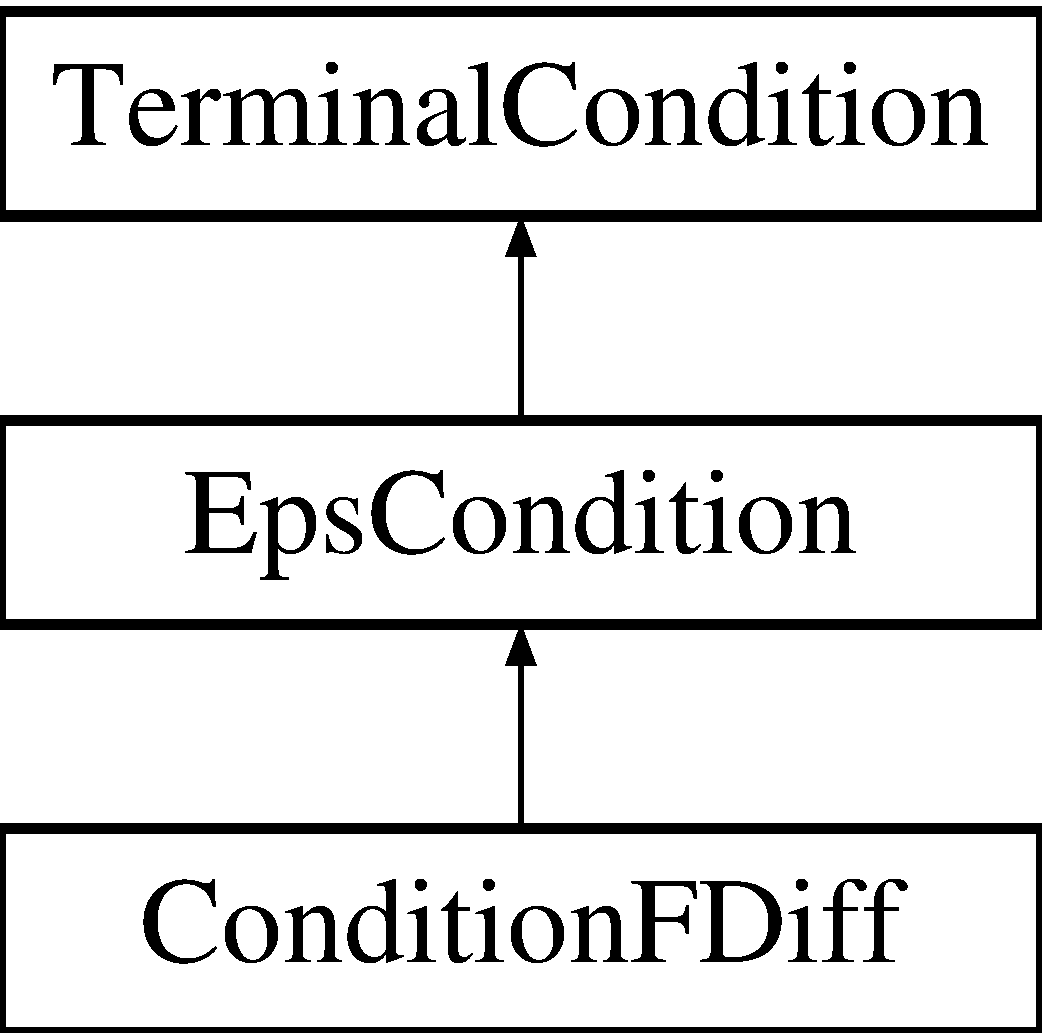
\includegraphics[height=3.000000cm]{class_condition_f_diff}
\end{center}
\end{figure}
\subsection*{Public Member Functions}
\begin{DoxyCompactItemize}
\item 
\mbox{\Hypertarget{class_condition_f_diff_af123e2b22ecad36fe88f3eba2a9ec3b6}\label{class_condition_f_diff_af123e2b22ecad36fe88f3eba2a9ec3b6}} 
\hyperlink{class_condition_f_diff_af123e2b22ecad36fe88f3eba2a9ec3b6}{Condition\+F\+Diff} (double \+\_\+eps)
\begin{DoxyCompactList}\small\item\em constructor \end{DoxyCompactList}\item 
\mbox{\Hypertarget{class_condition_f_diff_aebe3f77b561340000aebf0c97bd71144}\label{class_condition_f_diff_aebe3f77b561340000aebf0c97bd71144}} 
virtual \hyperlink{class_condition_f_diff_aebe3f77b561340000aebf0c97bd71144}{$\sim$\+Condition\+F\+Diff} ()
\begin{DoxyCompactList}\small\item\em destructor \end{DoxyCompactList}\item 
virtual bool \hyperlink{class_condition_f_diff_a31b06f62d08ab7c2ec1b011148889aab}{Stop} (std\+::shared\+\_\+ptr$<$ \hyperlink{class_function}{Function} $>$ F, const std\+::vector$<$ \hyperlink{classv_point}{v\+Point} $>$ \&Approx, const std\+::vector$<$ double $>$ \&Evals) const override
\item 
\mbox{\Hypertarget{class_condition_f_diff_af632ec588748eeb234bd1df7e95f74ea}\label{class_condition_f_diff_af632ec588748eeb234bd1df7e95f74ea}} 
virtual void \hyperlink{class_condition_f_diff_af632ec588748eeb234bd1df7e95f74ea}{Info} () const
\begin{DoxyCompactList}\small\item\em writes the name of the condition and the current value of epsilon \end{DoxyCompactList}\end{DoxyCompactItemize}
\subsection*{Additional Inherited Members}


\subsection{Detailed Description}
\hypertarget{function_8h_DESCRIPTION}{}\subsection{D\+E\+S\+C\+R\+I\+P\+T\+I\+ON}\label{function_8h_DESCRIPTION}
\hyperlink{class_condition_f_diff}{Condition\+F\+Diff} class is derived from \hyperlink{class_eps_condition}{Eps\+Condition} and represents a terminal condition based on the current value between the function evaluations of the last two approximations. 

\subsection{Member Function Documentation}
\mbox{\Hypertarget{class_condition_f_diff_a31b06f62d08ab7c2ec1b011148889aab}\label{class_condition_f_diff_a31b06f62d08ab7c2ec1b011148889aab}} 
\index{Condition\+F\+Diff@{Condition\+F\+Diff}!Stop@{Stop}}
\index{Stop@{Stop}!Condition\+F\+Diff@{Condition\+F\+Diff}}
\subsubsection{\texorpdfstring{Stop()}{Stop()}}
{\footnotesize\ttfamily bool Condition\+F\+Diff\+::\+Stop (\begin{DoxyParamCaption}\item[{std\+::shared\+\_\+ptr$<$ \hyperlink{class_function}{Function} $>$}]{F,  }\item[{const std\+::vector$<$ \hyperlink{classv_point}{v\+Point} $>$ \&}]{Approx,  }\item[{const std\+::vector$<$ double $>$ \&}]{Evals }\end{DoxyParamCaption}) const\hspace{0.3cm}{\ttfamily [override]}, {\ttfamily [virtual]}}

Overrides \hyperlink{class_terminal_condition_ad6294bf2bd6f5e2c6164e461c24d3198}{Terminal\+Condition\+::\+Stop} \begin{DoxyReturn}{Returns}
T\+R\+UE if the absolute value of the difference of the function evaluations of the two last approximations is less than epsilon and F\+A\+L\+SE otherwise 
\end{DoxyReturn}


Reimplemented from \hyperlink{class_terminal_condition_ad6294bf2bd6f5e2c6164e461c24d3198}{Terminal\+Condition}.



The documentation for this class was generated from the following files\+:\begin{DoxyCompactItemize}
\item 
condition\+\_\+f\+\_\+difference.\+h\item 
condition\+\_\+f\+\_\+difference.\+cpp\end{DoxyCompactItemize}

\hypertarget{class_condition_grad}{}\section{Condition\+Grad Class Reference}
\label{class_condition_grad}\index{Condition\+Grad@{Condition\+Grad}}


{\ttfamily \#include $<$condition\+\_\+grad.\+h$>$}

Inheritance diagram for Condition\+Grad\+:\begin{figure}[H]
\begin{center}
\leavevmode
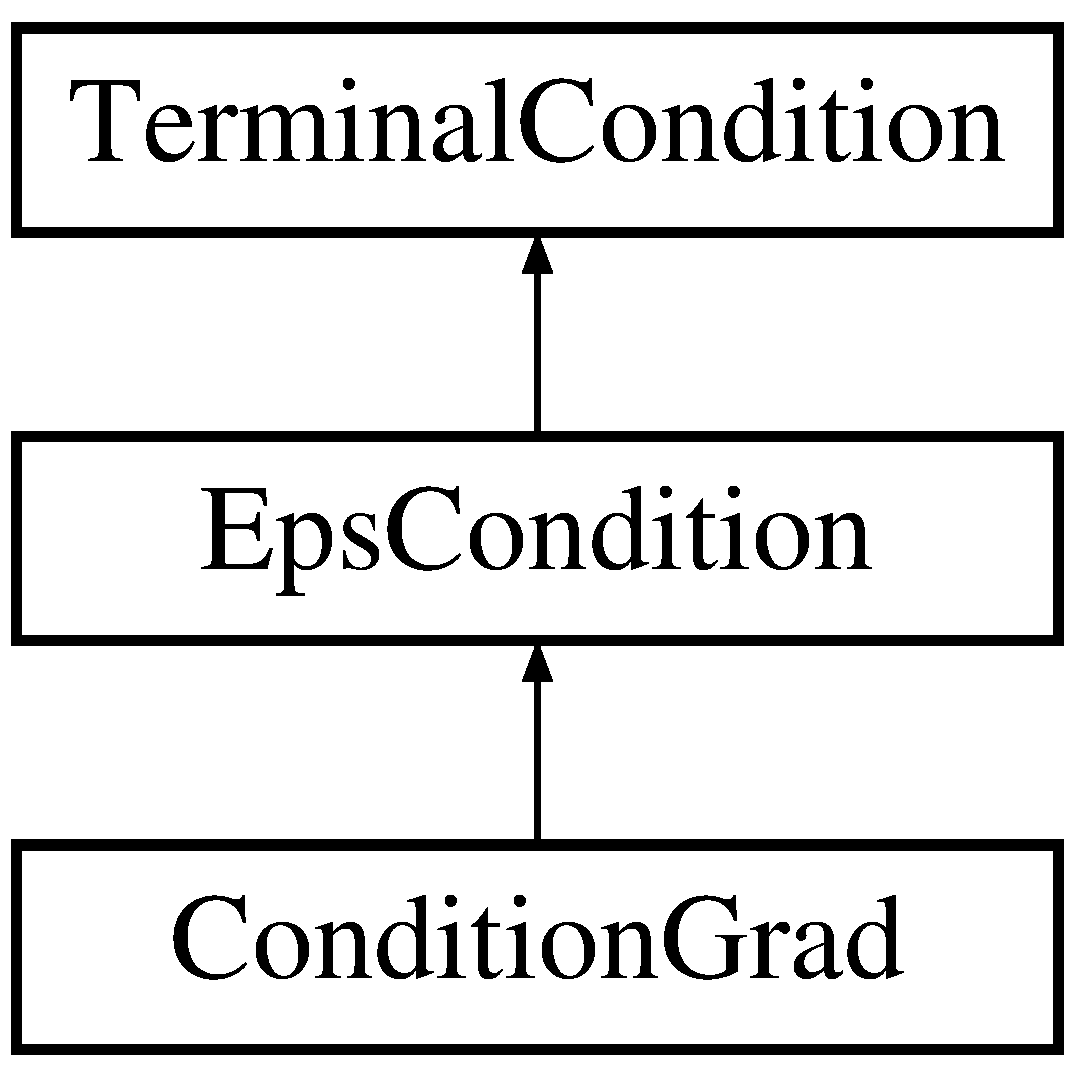
\includegraphics[height=3.000000cm]{class_condition_grad}
\end{center}
\end{figure}
\subsection*{Public Member Functions}
\begin{DoxyCompactItemize}
\item 
\mbox{\Hypertarget{class_condition_grad_a117455621eed050b982af3797e4ae232}\label{class_condition_grad_a117455621eed050b982af3797e4ae232}} 
\hyperlink{class_condition_grad_a117455621eed050b982af3797e4ae232}{Condition\+Grad} (double \+\_\+eps)
\begin{DoxyCompactList}\small\item\em constructor \end{DoxyCompactList}\item 
\mbox{\Hypertarget{class_condition_grad_a8320f7ec520c5a8a3f76981faccba3a8}\label{class_condition_grad_a8320f7ec520c5a8a3f76981faccba3a8}} 
\hyperlink{class_condition_grad_a8320f7ec520c5a8a3f76981faccba3a8}{$\sim$\+Condition\+Grad} ()
\begin{DoxyCompactList}\small\item\em destructor \end{DoxyCompactList}\item 
virtual bool \hyperlink{class_condition_grad_a28d97a0d0291b24976d4499b904190a7}{Stop} (std\+::shared\+\_\+ptr$<$ \hyperlink{class_function}{Function} $>$ F, const std\+::vector$<$ \hyperlink{classv_point}{v\+Point} $>$ \&Approx, const std\+::vector$<$ double $>$ \&Evals) const override
\item 
\mbox{\Hypertarget{class_condition_grad_a76f405067bfa70754c77dfadbaad5d3e}\label{class_condition_grad_a76f405067bfa70754c77dfadbaad5d3e}} 
virtual void \hyperlink{class_condition_grad_a76f405067bfa70754c77dfadbaad5d3e}{Info} () const
\begin{DoxyCompactList}\small\item\em writes the name of the condition and the current value of epsilon \end{DoxyCompactList}\end{DoxyCompactItemize}
\subsection*{Additional Inherited Members}


\subsection{Detailed Description}
\hypertarget{function_8h_DESCRIPTION}{}\subsection{D\+E\+S\+C\+R\+I\+P\+T\+I\+ON}\label{function_8h_DESCRIPTION}
Conditio\+Grad class is derived from \hyperlink{class_eps_condition}{Eps\+Condition} and represents a terminal condition based on the current value of the gradient of the function in the last approximation. 

\subsection{Member Function Documentation}
\mbox{\Hypertarget{class_condition_grad_a28d97a0d0291b24976d4499b904190a7}\label{class_condition_grad_a28d97a0d0291b24976d4499b904190a7}} 
\index{Condition\+Grad@{Condition\+Grad}!Stop@{Stop}}
\index{Stop@{Stop}!Condition\+Grad@{Condition\+Grad}}
\subsubsection{\texorpdfstring{Stop()}{Stop()}}
{\footnotesize\ttfamily bool Condition\+Grad\+::\+Stop (\begin{DoxyParamCaption}\item[{std\+::shared\+\_\+ptr$<$ \hyperlink{class_function}{Function} $>$}]{F,  }\item[{const std\+::vector$<$ \hyperlink{classv_point}{v\+Point} $>$ \&}]{Approx,  }\item[{const std\+::vector$<$ double $>$ \&}]{Evals }\end{DoxyParamCaption}) const\hspace{0.3cm}{\ttfamily [override]}, {\ttfamily [virtual]}}

Overrides \hyperlink{class_terminal_condition_ad6294bf2bd6f5e2c6164e461c24d3198}{Terminal\+Condition\+::\+Stop}. \begin{DoxyReturn}{Returns}
T\+R\+UE if the absolute value of the gradient of the function for the last approximation is less than epsilon and F\+A\+L\+SE otherwise. 
\end{DoxyReturn}


Reimplemented from \hyperlink{class_terminal_condition_ad6294bf2bd6f5e2c6164e461c24d3198}{Terminal\+Condition}.



The documentation for this class was generated from the following files\+:\begin{DoxyCompactItemize}
\item 
condition\+\_\+grad.\+h\item 
condition\+\_\+grad.\+cpp\end{DoxyCompactItemize}

\hypertarget{class_condition_improvement}{}\section{Condition\+Improvement Class Reference}
\label{class_condition_improvement}\index{Condition\+Improvement@{Condition\+Improvement}}


{\ttfamily \#include $<$condition\+\_\+improvement.\+h$>$}

Inheritance diagram for Condition\+Improvement\+:\begin{figure}[H]
\begin{center}
\leavevmode
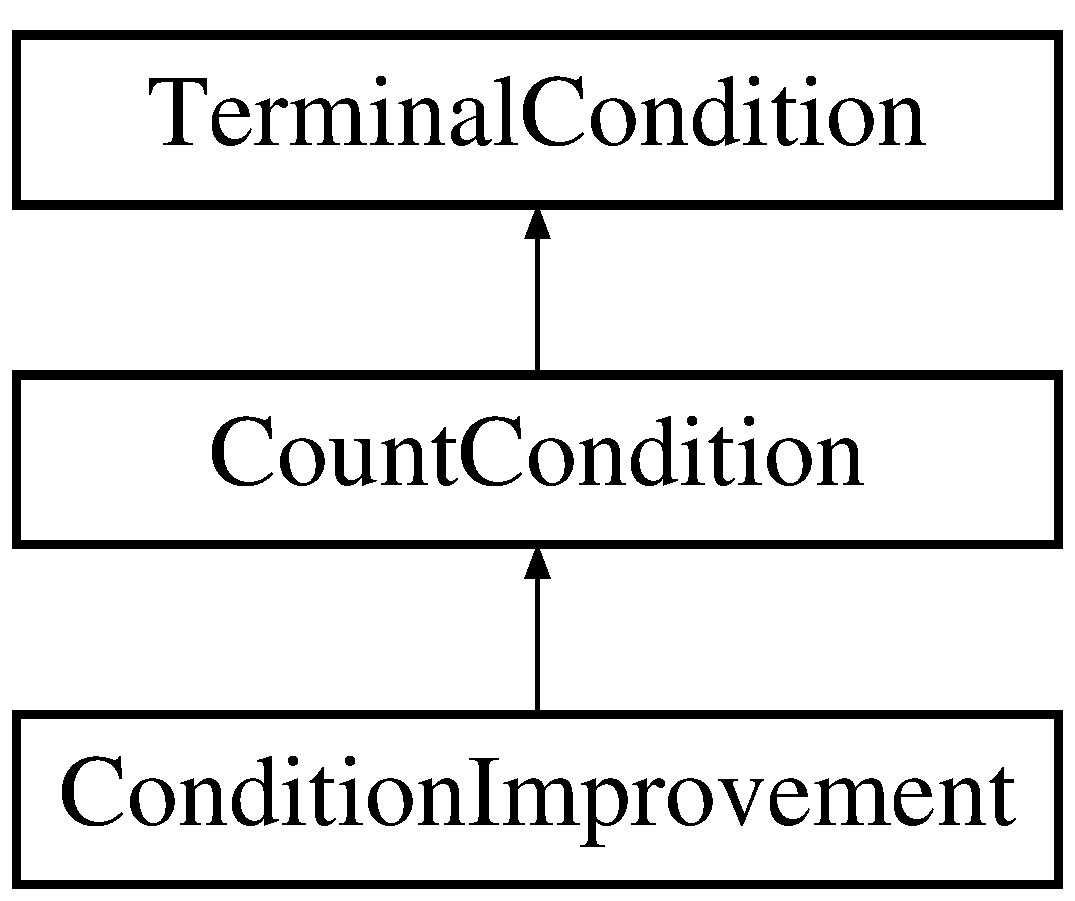
\includegraphics[height=3.000000cm]{class_condition_improvement}
\end{center}
\end{figure}
\subsection*{Public Member Functions}
\begin{DoxyCompactItemize}
\item 
\mbox{\Hypertarget{class_condition_improvement_aeff76aebcc0ce426a5dcd519547785be}\label{class_condition_improvement_aeff76aebcc0ce426a5dcd519547785be}} 
\hyperlink{class_condition_improvement_aeff76aebcc0ce426a5dcd519547785be}{Condition\+Improvement} (int \+\_\+mcount)
\begin{DoxyCompactList}\small\item\em constructor \end{DoxyCompactList}\item 
\mbox{\Hypertarget{class_condition_improvement_a1148c246d35ac61028db95d8c9289427}\label{class_condition_improvement_a1148c246d35ac61028db95d8c9289427}} 
\hyperlink{class_condition_improvement_a1148c246d35ac61028db95d8c9289427}{$\sim$\+Condition\+Improvement} ()
\begin{DoxyCompactList}\small\item\em destructor \end{DoxyCompactList}\item 
virtual bool \hyperlink{class_condition_improvement_a012d8db22fd6fcf8a71ab0fb5ecc1940}{Stop} (std\+::shared\+\_\+ptr$<$ \hyperlink{class_function}{Function} $>$ F, const std\+::vector$<$ \hyperlink{classv_point}{v\+Point} $>$ \&Approx, const std\+::vector$<$ double $>$ \&Evals) const override
\item 
\mbox{\Hypertarget{class_condition_improvement_a88b5dfa7c724f8d75276d4a65eb1f398}\label{class_condition_improvement_a88b5dfa7c724f8d75276d4a65eb1f398}} 
virtual void \hyperlink{class_condition_improvement_a88b5dfa7c724f8d75276d4a65eb1f398}{Info} () const
\begin{DoxyCompactList}\small\item\em writes the name of the condition and the current value of \end{DoxyCompactList}\end{DoxyCompactItemize}


\subsection{Detailed Description}
\hypertarget{function_8h_DESCRIPTION}{}\subsection{D\+E\+S\+C\+R\+I\+P\+T\+I\+ON}\label{function_8h_DESCRIPTION}
\hyperlink{class_condition_improvement}{Condition\+Improvement} class is derived from \hyperlink{class_count_condition}{Count\+Condition} and represents a terminal condition based with the method of termination based on the number of failures to improve the current approximation. 

\subsection{Member Function Documentation}
\mbox{\Hypertarget{class_condition_improvement_a012d8db22fd6fcf8a71ab0fb5ecc1940}\label{class_condition_improvement_a012d8db22fd6fcf8a71ab0fb5ecc1940}} 
\index{Condition\+Improvement@{Condition\+Improvement}!Stop@{Stop}}
\index{Stop@{Stop}!Condition\+Improvement@{Condition\+Improvement}}
\subsubsection{\texorpdfstring{Stop()}{Stop()}}
{\footnotesize\ttfamily bool Condition\+Improvement\+::\+Stop (\begin{DoxyParamCaption}\item[{std\+::shared\+\_\+ptr$<$ \hyperlink{class_function}{Function} $>$}]{F,  }\item[{const std\+::vector$<$ \hyperlink{classv_point}{v\+Point} $>$ \&}]{Approx,  }\item[{const std\+::vector$<$ double $>$ \&}]{Evals }\end{DoxyParamCaption}) const\hspace{0.3cm}{\ttfamily [override]}, {\ttfamily [virtual]}}

Overrides Terminal\+Condtion\+::\+Stop \begin{DoxyReturn}{Returns}
F\+A\+L\+SE if in the last Count\+Condition\+::max\+\_\+count of iterations the approximation was not improved and T\+R\+UE otherwise 
\end{DoxyReturn}


Reimplemented from \hyperlink{class_terminal_condition_ad6294bf2bd6f5e2c6164e461c24d3198}{Terminal\+Condition}.



The documentation for this class was generated from the following files\+:\begin{DoxyCompactItemize}
\item 
condition\+\_\+improvement.\+h\item 
condition\+\_\+improvement.\+cpp\end{DoxyCompactItemize}

\hypertarget{class_condition_iter}{}\section{Condition\+Iter Class Reference}
\label{class_condition_iter}\index{Condition\+Iter@{Condition\+Iter}}


{\ttfamily \#include $<$condition\+\_\+iter.\+h$>$}

Inheritance diagram for Condition\+Iter\+:\begin{figure}[H]
\begin{center}
\leavevmode
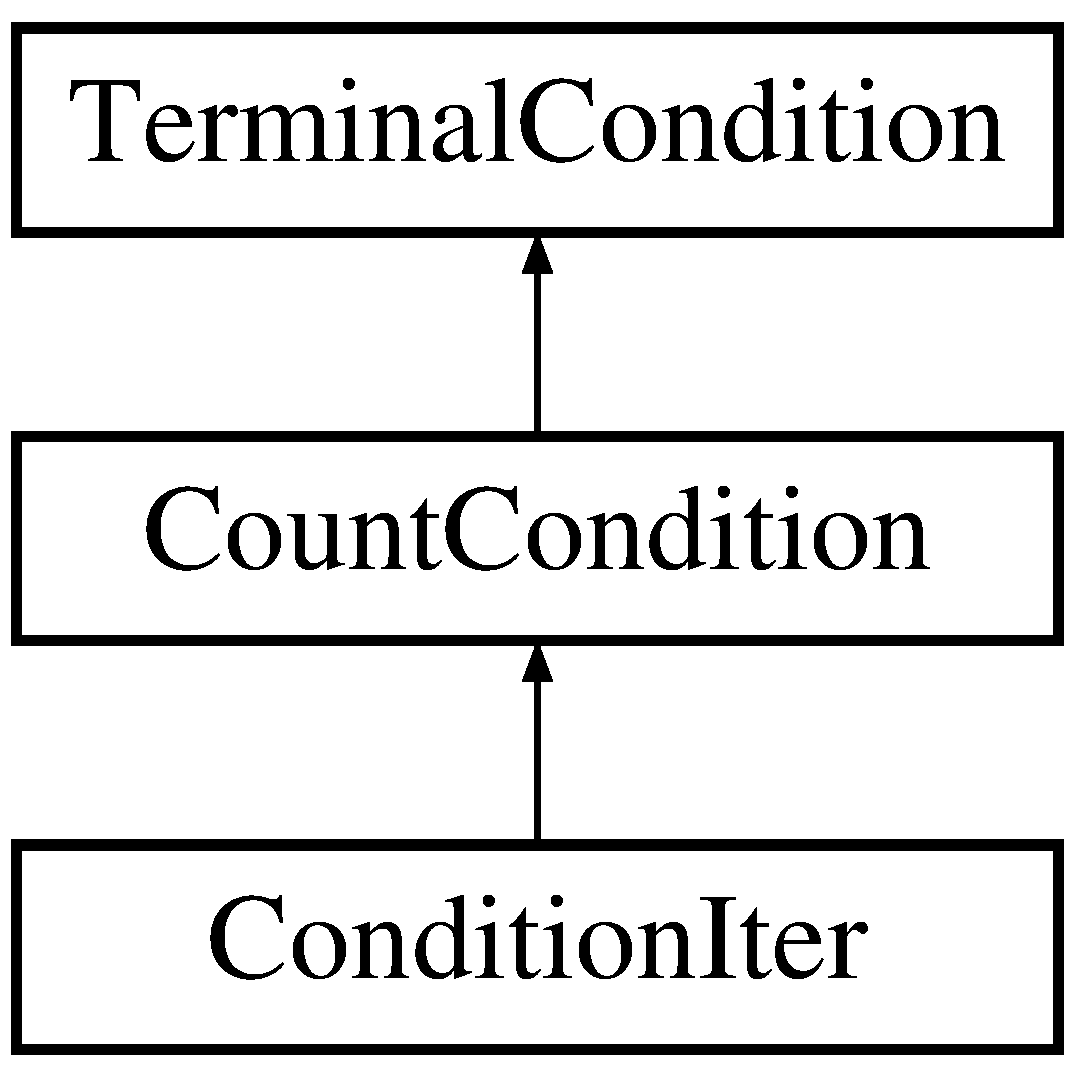
\includegraphics[height=3.000000cm]{class_condition_iter}
\end{center}
\end{figure}
\subsection*{Public Member Functions}
\begin{DoxyCompactItemize}
\item 
\mbox{\Hypertarget{class_condition_iter_a062d71109b94174f2efa1bab3fb0701d}\label{class_condition_iter_a062d71109b94174f2efa1bab3fb0701d}} 
\hyperlink{class_condition_iter_a062d71109b94174f2efa1bab3fb0701d}{Condition\+Iter} (int \+\_\+mcount)
\begin{DoxyCompactList}\small\item\em constructor \end{DoxyCompactList}\item 
virtual bool \hyperlink{class_condition_iter_af9de25d536e5a9af7bd711e569356533}{Stop} (std\+::shared\+\_\+ptr$<$ \hyperlink{class_function}{Function} $>$ F, const std\+::vector$<$ \hyperlink{classv_point}{v\+Point} $>$ \&Approx, const std\+::vector$<$ double $>$ \&Evals) const override
\item 
\mbox{\Hypertarget{class_condition_iter_acc2c4303cd4bbc84abb9619af2f74e5c}\label{class_condition_iter_acc2c4303cd4bbc84abb9619af2f74e5c}} 
virtual void \hyperlink{class_condition_iter_acc2c4303cd4bbc84abb9619af2f74e5c}{Info} () const
\begin{DoxyCompactList}\small\item\em writes the name of the method and the current value of maximum count of iterations \end{DoxyCompactList}\end{DoxyCompactItemize}


\subsection{Detailed Description}
\hypertarget{function_8h_DESCRIPTION}{}\subsection{D\+E\+S\+C\+R\+I\+P\+T\+I\+ON}\label{function_8h_DESCRIPTION}
\hyperlink{class_condition_iter}{Condition\+Iter} class is derived from \hyperlink{class_count_condition}{Count\+Condition} and represents a terminal condition based on the current number of iterations. 

\subsection{Member Function Documentation}
\mbox{\Hypertarget{class_condition_iter_af9de25d536e5a9af7bd711e569356533}\label{class_condition_iter_af9de25d536e5a9af7bd711e569356533}} 
\index{Condition\+Iter@{Condition\+Iter}!Stop@{Stop}}
\index{Stop@{Stop}!Condition\+Iter@{Condition\+Iter}}
\subsubsection{\texorpdfstring{Stop()}{Stop()}}
{\footnotesize\ttfamily bool Condition\+Iter\+::\+Stop (\begin{DoxyParamCaption}\item[{std\+::shared\+\_\+ptr$<$ \hyperlink{class_function}{Function} $>$}]{F,  }\item[{const std\+::vector$<$ \hyperlink{classv_point}{v\+Point} $>$ \&}]{Approx,  }\item[{const std\+::vector$<$ double $>$ \&}]{Evals }\end{DoxyParamCaption}) const\hspace{0.3cm}{\ttfamily [override]}, {\ttfamily [virtual]}}

Overrides \hyperlink{class_terminal_condition_ad6294bf2bd6f5e2c6164e461c24d3198}{Terminal\+Condition\+::\+Stop} \begin{DoxyReturn}{Returns}
T\+R\+UE if the number of iteration exceeds the maximum count and F\+A\+L\+SE otherwise 
\end{DoxyReturn}


Reimplemented from \hyperlink{class_terminal_condition_ad6294bf2bd6f5e2c6164e461c24d3198}{Terminal\+Condition}.



The documentation for this class was generated from the following files\+:\begin{DoxyCompactItemize}
\item 
condition\+\_\+iter.\+h\item 
condition\+\_\+iter.\+cpp\end{DoxyCompactItemize}

\hypertarget{class_condition_x_diff}{}\section{Condition\+X\+Diff Class Reference}
\label{class_condition_x_diff}\index{Condition\+X\+Diff@{Condition\+X\+Diff}}


{\ttfamily \#include $<$condition\+\_\+x\+\_\+difference.\+h$>$}

Inheritance diagram for Condition\+X\+Diff\+:\begin{figure}[H]
\begin{center}
\leavevmode
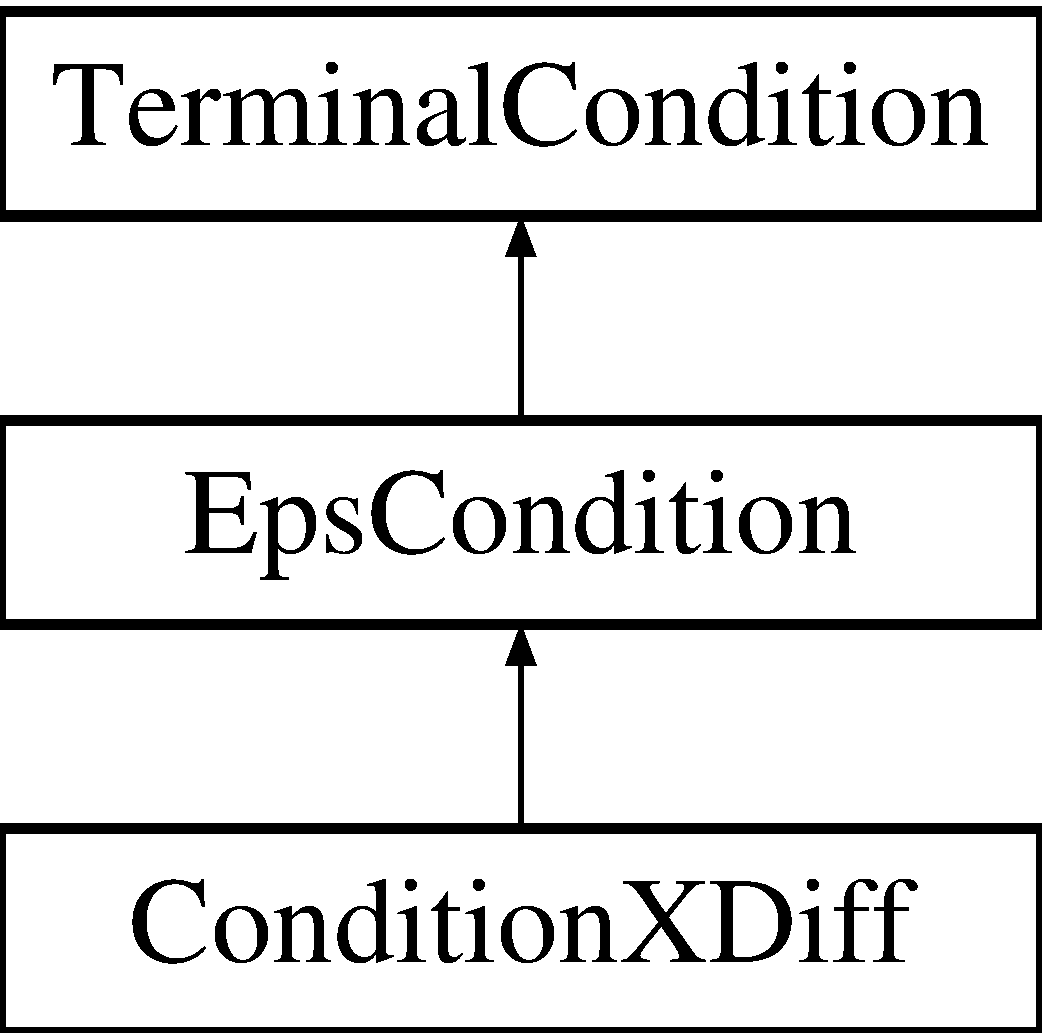
\includegraphics[height=3.000000cm]{class_condition_x_diff}
\end{center}
\end{figure}
\subsection*{Public Member Functions}
\begin{DoxyCompactItemize}
\item 
\mbox{\Hypertarget{class_condition_x_diff_a9a4c11adfbc93943c02c5ad778792467}\label{class_condition_x_diff_a9a4c11adfbc93943c02c5ad778792467}} 
\hyperlink{class_condition_x_diff_a9a4c11adfbc93943c02c5ad778792467}{Condition\+X\+Diff} (double \+\_\+eps)
\begin{DoxyCompactList}\small\item\em constructor \end{DoxyCompactList}\item 
\mbox{\Hypertarget{class_condition_x_diff_addb0a5448d4424e8bdacc31a0674b0b5}\label{class_condition_x_diff_addb0a5448d4424e8bdacc31a0674b0b5}} 
virtual \hyperlink{class_condition_x_diff_addb0a5448d4424e8bdacc31a0674b0b5}{$\sim$\+Condition\+X\+Diff} ()
\begin{DoxyCompactList}\small\item\em destructor \end{DoxyCompactList}\item 
virtual bool \hyperlink{class_condition_x_diff_a375e80eb4b88db5c2823a7d4efe20972}{Stop} (std\+::shared\+\_\+ptr$<$ \hyperlink{class_function}{Function} $>$ F, const std\+::vector$<$ \hyperlink{classv_point}{v\+Point} $>$ \&Approx, const std\+::vector$<$ double $>$ \&Evals) const override
\item 
\mbox{\Hypertarget{class_condition_x_diff_a90e346147a31dafdf5e79809efc6babd}\label{class_condition_x_diff_a90e346147a31dafdf5e79809efc6babd}} 
virtual void \hyperlink{class_condition_x_diff_a90e346147a31dafdf5e79809efc6babd}{Info} () const
\begin{DoxyCompactList}\small\item\em writes the name of the condition and the current value of epsilon \end{DoxyCompactList}\end{DoxyCompactItemize}
\subsection*{Additional Inherited Members}


\subsection{Detailed Description}
\hypertarget{function_8h_DESCRIPTION}{}\subsection{D\+E\+S\+C\+R\+I\+P\+T\+I\+ON}\label{function_8h_DESCRIPTION}
\hyperlink{class_condition_x_diff}{Condition\+X\+Diff} class is derived from \hyperlink{class_eps_condition}{Eps\+Condition} and represents a terminal condition based on the current value of the norm of the difference between the last two approximations. 

\subsection{Member Function Documentation}
\mbox{\Hypertarget{class_condition_x_diff_a375e80eb4b88db5c2823a7d4efe20972}\label{class_condition_x_diff_a375e80eb4b88db5c2823a7d4efe20972}} 
\index{Condition\+X\+Diff@{Condition\+X\+Diff}!Stop@{Stop}}
\index{Stop@{Stop}!Condition\+X\+Diff@{Condition\+X\+Diff}}
\subsubsection{\texorpdfstring{Stop()}{Stop()}}
{\footnotesize\ttfamily bool Condition\+X\+Diff\+::\+Stop (\begin{DoxyParamCaption}\item[{std\+::shared\+\_\+ptr$<$ \hyperlink{class_function}{Function} $>$}]{F,  }\item[{const std\+::vector$<$ \hyperlink{classv_point}{v\+Point} $>$ \&}]{Approx,  }\item[{const std\+::vector$<$ double $>$ \&}]{Evals }\end{DoxyParamCaption}) const\hspace{0.3cm}{\ttfamily [override]}, {\ttfamily [virtual]}}

Overrides \hyperlink{class_terminal_condition_ad6294bf2bd6f5e2c6164e461c24d3198}{Terminal\+Condition\+::\+Stop}. \begin{DoxyReturn}{Returns}
T\+R\+UE if the norm of the difference betweeen the two last approximations is less than epsilon and F\+A\+L\+SE otherwise. 
\end{DoxyReturn}


Reimplemented from \hyperlink{class_terminal_condition_ad6294bf2bd6f5e2c6164e461c24d3198}{Terminal\+Condition}.



The documentation for this class was generated from the following files\+:\begin{DoxyCompactItemize}
\item 
condition\+\_\+x\+\_\+difference.\+h\item 
condition\+\_\+x\+\_\+difference.\+cpp\end{DoxyCompactItemize}

\hypertarget{class_count_condition}{}\section{Count\+Condition Class Reference}
\label{class_count_condition}\index{Count\+Condition@{Count\+Condition}}


{\ttfamily \#include $<$count\+\_\+condition.\+h$>$}

Inheritance diagram for Count\+Condition\+:\begin{figure}[H]
\begin{center}
\leavevmode
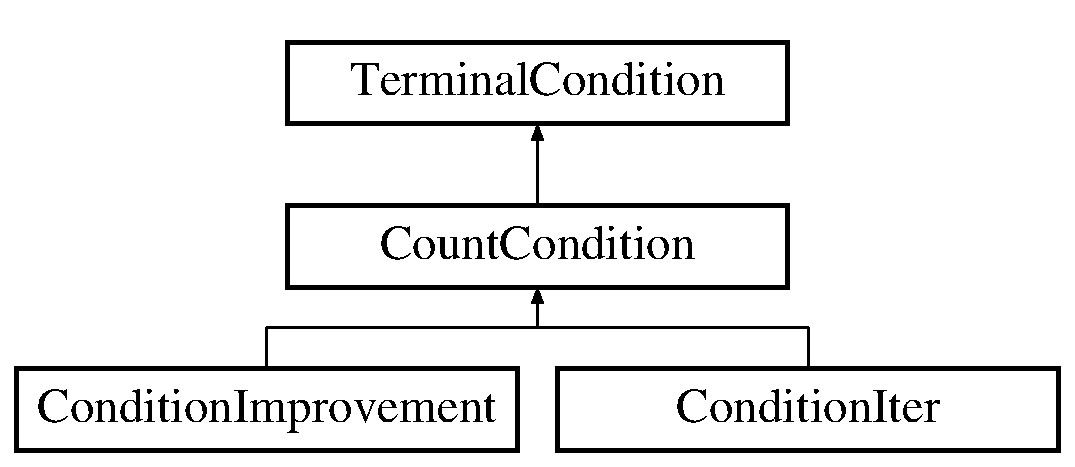
\includegraphics[height=3.000000cm]{class_count_condition}
\end{center}
\end{figure}
\subsection*{Public Member Functions}
\begin{DoxyCompactItemize}
\item 
\mbox{\Hypertarget{class_count_condition_a5de1b537356b81f9deae0092acaa1f6c}\label{class_count_condition_a5de1b537356b81f9deae0092acaa1f6c}} 
\hyperlink{class_count_condition_a5de1b537356b81f9deae0092acaa1f6c}{Count\+Condition} (int \+\_\+mcount)
\begin{DoxyCompactList}\small\item\em constructor that sets the main parameter of the condition \end{DoxyCompactList}\item 
\mbox{\Hypertarget{class_count_condition_a64dd5e9e032acc504a780f1110e369d3}\label{class_count_condition_a64dd5e9e032acc504a780f1110e369d3}} 
virtual \hyperlink{class_count_condition_a64dd5e9e032acc504a780f1110e369d3}{$\sim$\+Count\+Condition} ()
\begin{DoxyCompactList}\small\item\em destructor \end{DoxyCompactList}\item 
\mbox{\Hypertarget{class_count_condition_a7652f4ce1530378d617b2700b984a3a6}\label{class_count_condition_a7652f4ce1530378d617b2700b984a3a6}} 
bool \hyperlink{class_count_condition_a7652f4ce1530378d617b2700b984a3a6}{Set\+Max\+Count} (int \+\_\+mcount)
\begin{DoxyCompactList}\small\item\em sets the maximum count of the event to a given value with argument validation. \end{DoxyCompactList}\item 
\mbox{\Hypertarget{class_count_condition_ae7f23cc8b64ae574691fd62af2e2091d}\label{class_count_condition_ae7f23cc8b64ae574691fd62af2e2091d}} 
int \hyperlink{class_count_condition_ae7f23cc8b64ae574691fd62af2e2091d}{Get\+Max\+Count} () const
\begin{DoxyCompactList}\small\item\em returns the maximum count \end{DoxyCompactList}\end{DoxyCompactItemize}


\subsection{Detailed Description}
\hypertarget{function_8h_DESCRIPTION}{}\subsection{D\+E\+S\+C\+R\+I\+P\+T\+I\+ON}\label{function_8h_DESCRIPTION}
The \hyperlink{class_count_condition}{Count\+Condition} class represents a \hyperlink{class_terminal_condition}{Terminal\+Condition} with an integer number as main parameter (the count of an event) 

The documentation for this class was generated from the following files\+:\begin{DoxyCompactItemize}
\item 
count\+\_\+condition.\+h\item 
count\+\_\+condition.\+cpp\end{DoxyCompactItemize}

\hypertarget{class_eps_condition}{}\section{Eps\+Condition Class Reference}
\label{class_eps_condition}\index{Eps\+Condition@{Eps\+Condition}}
Inheritance diagram for Eps\+Condition\+:\begin{figure}[H]
\begin{center}
\leavevmode
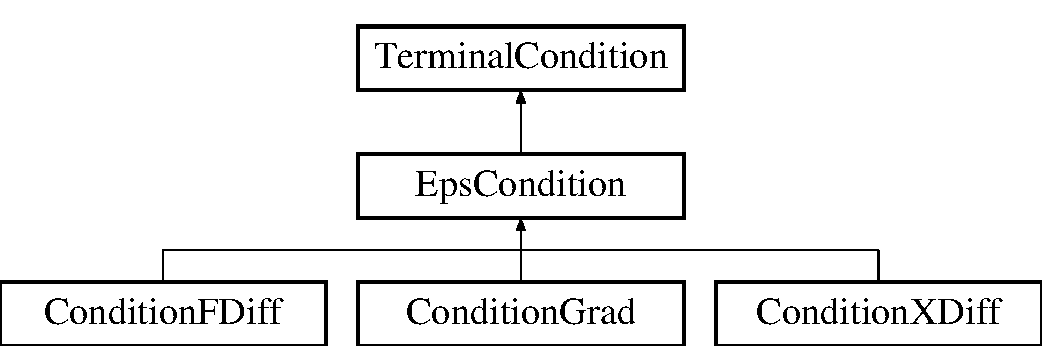
\includegraphics[height=3.000000cm]{class_eps_condition}
\end{center}
\end{figure}
\subsection*{Public Member Functions}
\begin{DoxyCompactItemize}
\item 
\mbox{\Hypertarget{class_eps_condition_ad6d567f401d6a5028a2d48c61f2ac3d8}\label{class_eps_condition_ad6d567f401d6a5028a2d48c61f2ac3d8}} 
\hyperlink{class_eps_condition_ad6d567f401d6a5028a2d48c61f2ac3d8}{Eps\+Condition} (double \+\_\+eps)
\begin{DoxyCompactList}\small\item\em constructor that sets the main parameter of the condition \end{DoxyCompactList}\item 
\mbox{\Hypertarget{class_eps_condition_a892b576e42fe950c0fea5a3afcf4ea69}\label{class_eps_condition_a892b576e42fe950c0fea5a3afcf4ea69}} 
virtual \hyperlink{class_eps_condition_a892b576e42fe950c0fea5a3afcf4ea69}{$\sim$\+Eps\+Condition} ()
\begin{DoxyCompactList}\small\item\em destructor \end{DoxyCompactList}\item 
\mbox{\Hypertarget{class_eps_condition_a8a0fd013059f6f45c1ecfe2a6f38ece7}\label{class_eps_condition_a8a0fd013059f6f45c1ecfe2a6f38ece7}} 
bool \hyperlink{class_eps_condition_a8a0fd013059f6f45c1ecfe2a6f38ece7}{Set\+Eps} (double \+\_\+eps)
\begin{DoxyCompactList}\small\item\em sets the main parameter of the condition with argument validation \end{DoxyCompactList}\item 
\mbox{\Hypertarget{class_eps_condition_a0b5c302ebf949287188abf368df4c2b8}\label{class_eps_condition_a0b5c302ebf949287188abf368df4c2b8}} 
double \hyperlink{class_eps_condition_a0b5c302ebf949287188abf368df4c2b8}{Get\+Eps} () const
\begin{DoxyCompactList}\small\item\em returns the main parameter of the condition \end{DoxyCompactList}\end{DoxyCompactItemize}
\subsection*{Protected Attributes}
\begin{DoxyCompactItemize}
\item 
\mbox{\Hypertarget{class_eps_condition_a43f4dafd1f2fd2b425a7a51a74f1551f}\label{class_eps_condition_a43f4dafd1f2fd2b425a7a51a74f1551f}} 
double \hyperlink{class_eps_condition_a43f4dafd1f2fd2b425a7a51a74f1551f}{epsilon}
\begin{DoxyCompactList}\small\item\em the main parameter of the condition (a double that is used in number comparison) \end{DoxyCompactList}\end{DoxyCompactItemize}


The documentation for this class was generated from the following files\+:\begin{DoxyCompactItemize}
\item 
eps\+\_\+condition.\+h\item 
eps\+\_\+condition.\+cpp\end{DoxyCompactItemize}

\hypertarget{class_function}{}\section{Function Class Reference}
\label{class_function}\index{Function@{Function}}
Inheritance diagram for Function\+:\begin{figure}[H]
\begin{center}
\leavevmode
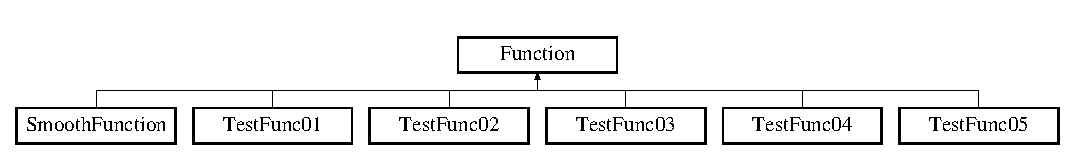
\includegraphics[height=1.696970cm]{class_function}
\end{center}
\end{figure}
\subsection*{Public Member Functions}
\begin{DoxyCompactItemize}
\item 
\hyperlink{class_function_a28c4db5ca9f2bbe27fd51ed0169bd2de}{Function} (std\+::shared\+\_\+ptr$<$ \hyperlink{class_area}{Area} $>$ \+\_\+domain)
\item 
virtual \hyperlink{class_function_a8697b2e490a4314a7ccbb17aea8ce537}{$\sim$\+Function} ()
\item 
virtual double \hyperlink{class_function_a8b9d55271a531b6f5bef09bfae0a23d9}{eval} (const \hyperlink{classv_point}{v\+Point} \&X) const =0
\item 
int \hyperlink{class_function_a531e81f5d7f7cafce7c211c08c3c7041}{Get\+Dim} () const
\item 
double \hyperlink{class_function_acc67abadb0c13fbe3a0cc96c65f2b55b}{operator()} (const \hyperlink{classv_point}{v\+Point} \&X) const
\item 
virtual void \hyperlink{class_function_a6915be18a065224ed73b1288c6125948}{Info} () const =0
\end{DoxyCompactItemize}
\subsection*{Protected Attributes}
\begin{DoxyCompactItemize}
\item 
\mbox{\Hypertarget{class_function_a809df8b9c6dc40e7853e96efa4756881}\label{class_function_a809df8b9c6dc40e7853e96efa4756881}} 
std\+::shared\+\_\+ptr$<$ \hyperlink{class_area}{Area} $>$ \hyperlink{class_function_a809df8b9c6dc40e7853e96efa4756881}{domain}
\begin{DoxyCompactList}\small\item\em the domain of the function (the area in which the function is defined) \end{DoxyCompactList}\end{DoxyCompactItemize}
\subsection*{Friends}
\begin{DoxyCompactItemize}
\item 
std\+::ostream \& \hyperlink{class_function_ada3899626dabeaf7910d55f156499baf}{operator$<$$<$} (std\+::ostream \&out, std\+::shared\+\_\+ptr$<$ \hyperlink{class_function}{Function} $>$ F)
\item 
double \hyperlink{class_function_a74f93e0ab18699467c6a96e4c500b256}{Calc\+Grad} (std\+::shared\+\_\+ptr$<$ \hyperlink{class_function}{Function} $>$ F, const \hyperlink{classv_point}{v\+Point} \&X, double delta)
\end{DoxyCompactItemize}


\subsection{Constructor \& Destructor Documentation}
\mbox{\Hypertarget{class_function_a28c4db5ca9f2bbe27fd51ed0169bd2de}\label{class_function_a28c4db5ca9f2bbe27fd51ed0169bd2de}} 
\index{Function@{Function}!Function@{Function}}
\index{Function@{Function}!Function@{Function}}
\subsubsection{\texorpdfstring{Function()}{Function()}}
{\footnotesize\ttfamily Function\+::\+Function (\begin{DoxyParamCaption}\item[{std\+::shared\+\_\+ptr$<$ \hyperlink{class_area}{Area} $>$}]{\+\_\+domain }\end{DoxyParamCaption})\hspace{0.3cm}{\ttfamily [inline]}}

constructor that sets the domain of the function 
\begin{DoxyParams}{Parameters}
{\em \+\_\+domain} & Domain of the function \\
\hline
\end{DoxyParams}
\mbox{\Hypertarget{class_function_a8697b2e490a4314a7ccbb17aea8ce537}\label{class_function_a8697b2e490a4314a7ccbb17aea8ce537}} 
\index{Function@{Function}!````~Function@{$\sim$\+Function}}
\index{````~Function@{$\sim$\+Function}!Function@{Function}}
\subsubsection{\texorpdfstring{$\sim$\+Function()}{~Function()}}
{\footnotesize\ttfamily virtual Function\+::$\sim$\+Function (\begin{DoxyParamCaption}{ }\end{DoxyParamCaption})\hspace{0.3cm}{\ttfamily [inline]}, {\ttfamily [virtual]}}

destructor of the class 

\subsection{Member Function Documentation}
\mbox{\Hypertarget{class_function_a8b9d55271a531b6f5bef09bfae0a23d9}\label{class_function_a8b9d55271a531b6f5bef09bfae0a23d9}} 
\index{Function@{Function}!eval@{eval}}
\index{eval@{eval}!Function@{Function}}
\subsubsection{\texorpdfstring{eval()}{eval()}}
{\footnotesize\ttfamily virtual double Function\+::eval (\begin{DoxyParamCaption}\item[{const \hyperlink{classv_point}{v\+Point} \&}]{X }\end{DoxyParamCaption}) const\hspace{0.3cm}{\ttfamily [pure virtual]}}

abstract method that returns the result of evaluation of the function in given point 
\begin{DoxyParams}{Parameters}
{\em X} & The point in which the function is evaluated \\
\hline
\end{DoxyParams}
\begin{DoxyReturn}{Returns}
double precision number which represents the result of the evaluation 
\end{DoxyReturn}


Implemented in \hyperlink{class_test_func01_a50b43b414345a790599ef55960a81cdb}{Test\+Func01}, \hyperlink{class_test_func02_af4cbebcbe8a7bd282f48ae7053c044b0}{Test\+Func02}, \hyperlink{class_test_func03_a76417746f25346a1de704bfcac3eba47}{Test\+Func03}, \hyperlink{class_test_func04_a8c4666904611a414b985d17661847ec7}{Test\+Func04}, and \hyperlink{class_test_func05_a2848dbb9b76d0db3a701ce69ec700923}{Test\+Func05}.

\mbox{\Hypertarget{class_function_a531e81f5d7f7cafce7c211c08c3c7041}\label{class_function_a531e81f5d7f7cafce7c211c08c3c7041}} 
\index{Function@{Function}!Get\+Dim@{Get\+Dim}}
\index{Get\+Dim@{Get\+Dim}!Function@{Function}}
\subsubsection{\texorpdfstring{Get\+Dim()}{GetDim()}}
{\footnotesize\ttfamily int Function\+::\+Get\+Dim (\begin{DoxyParamCaption}{ }\end{DoxyParamCaption}) const\hspace{0.3cm}{\ttfamily [inline]}}

returns the dimension of the function domain \begin{DoxyReturn}{Returns}
the domain dimension 
\end{DoxyReturn}
\mbox{\Hypertarget{class_function_a6915be18a065224ed73b1288c6125948}\label{class_function_a6915be18a065224ed73b1288c6125948}} 
\index{Function@{Function}!Info@{Info}}
\index{Info@{Info}!Function@{Function}}
\subsubsection{\texorpdfstring{Info()}{Info()}}
{\footnotesize\ttfamily virtual void Function\+::\+Info (\begin{DoxyParamCaption}{ }\end{DoxyParamCaption}) const\hspace{0.3cm}{\ttfamily [pure virtual]}}

abstract method that prints the formula of the function 

Implemented in \hyperlink{class_test_func01_a731cfb0260fe58f6eab02f11449737e0}{Test\+Func01}, \hyperlink{class_test_func02_abb39a10959e945371e662db3cd9d86ce}{Test\+Func02}, \hyperlink{class_test_func03_aab454f96f95f28f7ce1d58736d7fdf86}{Test\+Func03}, \hyperlink{class_test_func04_a7c2bf8c334c926cbfa464081e33ac30f}{Test\+Func04}, and \hyperlink{class_test_func05_a2a1c8696724c5195e92b4194d6205dcb}{Test\+Func05}.

\mbox{\Hypertarget{class_function_acc67abadb0c13fbe3a0cc96c65f2b55b}\label{class_function_acc67abadb0c13fbe3a0cc96c65f2b55b}} 
\index{Function@{Function}!operator()@{operator()}}
\index{operator()@{operator()}!Function@{Function}}
\subsubsection{\texorpdfstring{operator()()}{operator()()}}
{\footnotesize\ttfamily double Function\+::operator() (\begin{DoxyParamCaption}\item[{const \hyperlink{classv_point}{v\+Point} \&}]{X }\end{DoxyParamCaption}) const\hspace{0.3cm}{\ttfamily [inline]}}

returns the result of evaluation of the function in given point (equal to eval(\+X)) 
\begin{DoxyParams}{Parameters}
{\em X} & The point in which the function is evaluated \\
\hline
\end{DoxyParams}
\begin{DoxyReturn}{Returns}
double precision number which represents the result of the evaluation 
\end{DoxyReturn}


\subsection{Friends And Related Function Documentation}
\mbox{\Hypertarget{class_function_a74f93e0ab18699467c6a96e4c500b256}\label{class_function_a74f93e0ab18699467c6a96e4c500b256}} 
\index{Function@{Function}!Calc\+Grad@{Calc\+Grad}}
\index{Calc\+Grad@{Calc\+Grad}!Function@{Function}}
\subsubsection{\texorpdfstring{Calc\+Grad}{CalcGrad}}
{\footnotesize\ttfamily double Calc\+Grad (\begin{DoxyParamCaption}\item[{std\+::shared\+\_\+ptr$<$ \hyperlink{class_function}{Function} $>$}]{F,  }\item[{const \hyperlink{classv_point}{v\+Point} \&}]{X,  }\item[{double}]{delta }\end{DoxyParamCaption})\hspace{0.3cm}{\ttfamily [friend]}}

calculates gradient of the function F using formula\+: 1 / (2$\ast$dX) $\ast$ (F(X + dX) -\/ F(X -\/ dX)) \begin{DoxyReturn}{Returns}
double precision number which represents the result of the gradient calculation 
\end{DoxyReturn}
\mbox{\Hypertarget{class_function_ada3899626dabeaf7910d55f156499baf}\label{class_function_ada3899626dabeaf7910d55f156499baf}} 
\index{Function@{Function}!operator$<$$<$@{operator$<$$<$}}
\index{operator$<$$<$@{operator$<$$<$}!Function@{Function}}
\subsubsection{\texorpdfstring{operator$<$$<$}{operator<<}}
{\footnotesize\ttfamily std\+::ostream\& operator$<$$<$ (\begin{DoxyParamCaption}\item[{std\+::ostream \&}]{out,  }\item[{std\+::shared\+\_\+ptr$<$ \hyperlink{class_function}{Function} $>$}]{F }\end{DoxyParamCaption})\hspace{0.3cm}{\ttfamily [friend]}}

prints the formula of the function std\+::cout stream 
\begin{DoxyParams}{Parameters}
{\em out} & output stream \\
\hline
{\em F} & shared pointer to the function, which formula is to be printed \\
\hline
\end{DoxyParams}


The documentation for this class was generated from the following file\+:\begin{DoxyCompactItemize}
\item 
\hyperlink{function_8h}{function.\+h}\end{DoxyCompactItemize}

\hypertarget{class_n_cube}{}\section{N\+Cube Class Reference}
\label{class_n_cube}\index{N\+Cube@{N\+Cube}}


{\ttfamily \#include $<$ncube.\+h$>$}

Inheritance diagram for N\+Cube\+:\begin{figure}[H]
\begin{center}
\leavevmode
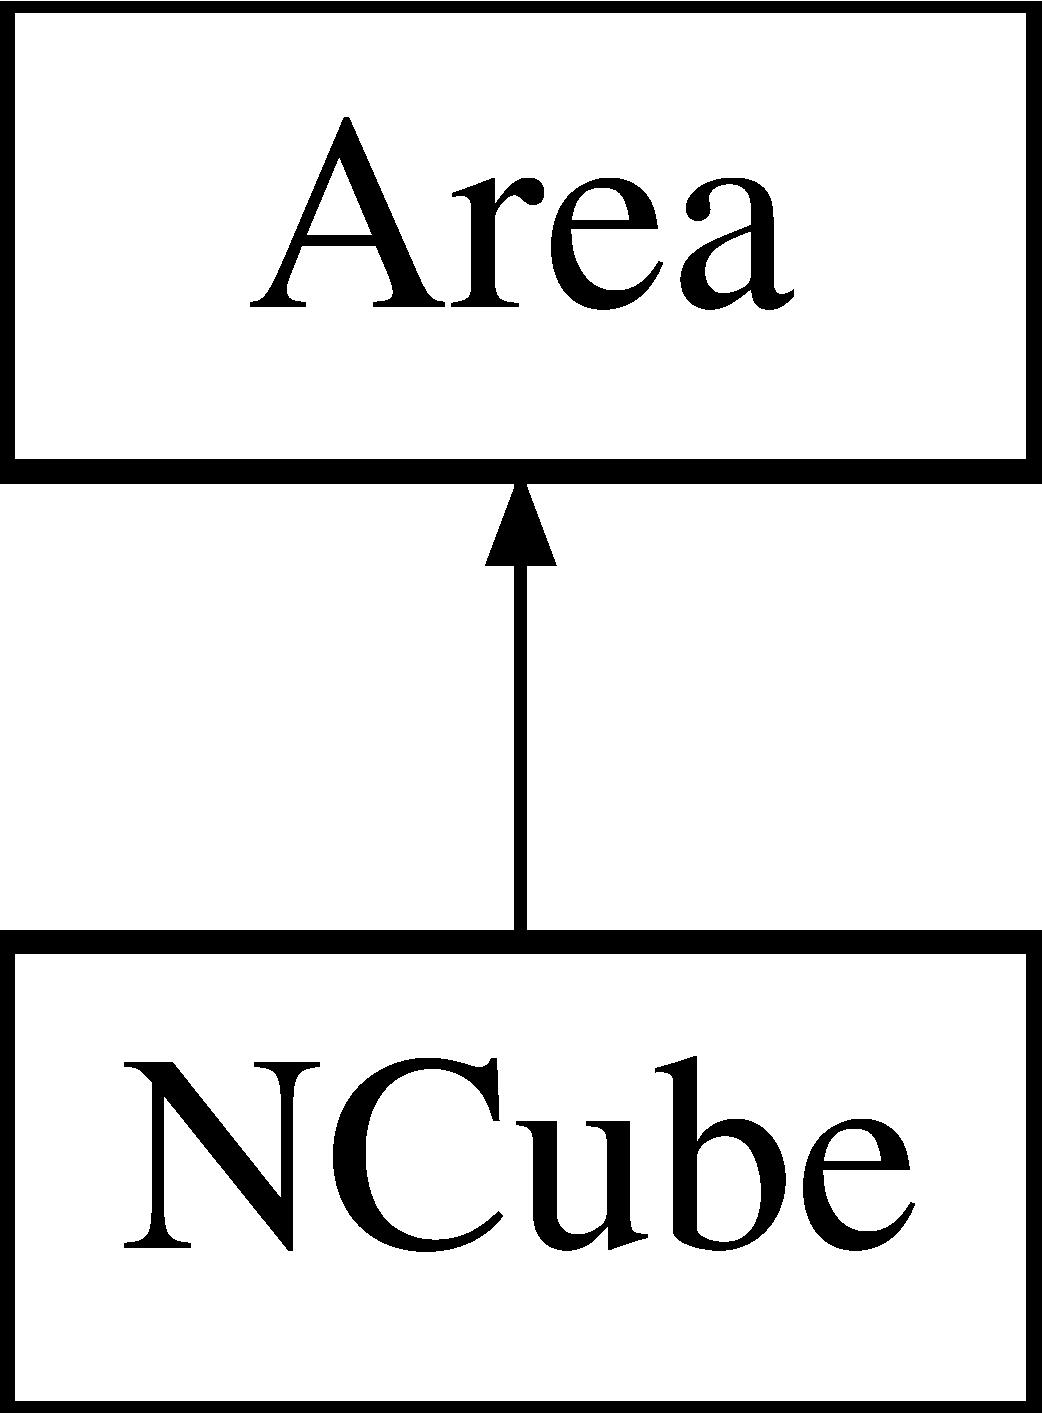
\includegraphics[height=2.000000cm]{class_n_cube}
\end{center}
\end{figure}
\subsection*{Public Member Functions}
\begin{DoxyCompactItemize}
\item 
\hyperlink{class_n_cube_ac5458bbe42846badcbd2100825a76556}{N\+Cube} (const Range\+Vec \&\+\_\+ranges)
\item 
\hyperlink{class_n_cube_a2eeaca555a32a13ed8fc58e2e83b1ec4}{N\+Cube} (int \+\_\+dim=2)
\item 
\hyperlink{class_n_cube_a6b4535debc936abca85e563f5b4e1d67}{N\+Cube} (std\+::vector$<$ double $>$ \&minimums, std\+::vector$<$ double $>$ \&maximums)
\item 
\mbox{\Hypertarget{class_n_cube_a7c2e9733c2a48e1c60397321166d688a}\label{class_n_cube_a7c2e9733c2a48e1c60397321166d688a}} 
virtual \hyperlink{class_n_cube_a7c2e9733c2a48e1c60397321166d688a}{$\sim$\+N\+Cube} ()
\begin{DoxyCompactList}\small\item\em destructor \end{DoxyCompactList}\item 
virtual bool \hyperlink{class_n_cube_a042595f5e33795b2b454c2da3e9f13e0}{In} (const \hyperlink{classv_point}{v\+Point} \&X) const
\item 
virtual \hyperlink{classv_point}{v\+Point} \hyperlink{class_n_cube_a44e37293282724b0454c4542fa001c60}{Random\+Point} () const
\item 
virtual std\+::shared\+\_\+ptr$<$ \hyperlink{class_area}{Area} $>$ \hyperlink{class_n_cube_a88be716167199c626d1c5063b6929303}{Sub\+Area} (const \hyperlink{classv_point}{v\+Point} \&X, double epsilon) const
\item 
\mbox{\Hypertarget{class_n_cube_a14a756408e6b20bb3537cc1e32f9032d}\label{class_n_cube_a14a756408e6b20bb3537cc1e32f9032d}} 
const \hyperlink{class_range}{Range} \& \hyperlink{class_n_cube_a14a756408e6b20bb3537cc1e32f9032d}{operator\mbox{[}$\,$\mbox{]}} (int index) const
\begin{DoxyCompactList}\small\item\em returns the range of the cube at given index \end{DoxyCompactList}\item 
\mbox{\Hypertarget{class_n_cube_a6018d8b57d76586cec10b6e4a2741e44}\label{class_n_cube_a6018d8b57d76586cec10b6e4a2741e44}} 
\hyperlink{class_range}{Range} \& \hyperlink{class_n_cube_a6018d8b57d76586cec10b6e4a2741e44}{operator\mbox{[}$\,$\mbox{]}} (int index)
\begin{DoxyCompactList}\small\item\em returns the range of the cube at given index \end{DoxyCompactList}\item 
\mbox{\Hypertarget{class_n_cube_a6e89fbd9fc41e833db790b6969b05e0e}\label{class_n_cube_a6e89fbd9fc41e833db790b6969b05e0e}} 
const \hyperlink{class_range}{Range} \& \hyperlink{class_n_cube_a6e89fbd9fc41e833db790b6969b05e0e}{at} (int index) const
\begin{DoxyCompactList}\small\item\em returns the range of the cube at given index but validates whether the index is in index range \end{DoxyCompactList}\item 
\mbox{\Hypertarget{class_n_cube_a4b10f642983c3c2d32f7b9c4ab5117a0}\label{class_n_cube_a4b10f642983c3c2d32f7b9c4ab5117a0}} 
\hyperlink{class_range}{Range} \& \hyperlink{class_n_cube_a4b10f642983c3c2d32f7b9c4ab5117a0}{at} (int index)
\begin{DoxyCompactList}\small\item\em returns the range of the cube at given index but validates whether the index is in index range \end{DoxyCompactList}\item 
\mbox{\Hypertarget{class_n_cube_aa7387e8654574bf3f4a0e32633516451}\label{class_n_cube_aa7387e8654574bf3f4a0e32633516451}} 
virtual void \hyperlink{class_n_cube_aa7387e8654574bf3f4a0e32633516451}{Info} () const
\begin{DoxyCompactList}\small\item\em writes the information about the cube and its ranges to std\+::cout \end{DoxyCompactList}\end{DoxyCompactItemize}
\subsection*{Additional Inherited Members}


\subsection{Detailed Description}
\hypertarget{function_8h_DESCRIPTION}{}\subsection{D\+E\+S\+C\+R\+I\+P\+T\+I\+ON}\label{function_8h_DESCRIPTION}
The \hyperlink{class_n_cube}{N\+Cube} class is derived from \hyperlink{class_area}{Area} and represents a multidimensional cube that consists of onedimensional ranges 

\subsection{Constructor \& Destructor Documentation}
\mbox{\Hypertarget{class_n_cube_ac5458bbe42846badcbd2100825a76556}\label{class_n_cube_ac5458bbe42846badcbd2100825a76556}} 
\index{N\+Cube@{N\+Cube}!N\+Cube@{N\+Cube}}
\index{N\+Cube@{N\+Cube}!N\+Cube@{N\+Cube}}
\subsubsection{\texorpdfstring{N\+Cube()}{NCube()}\hspace{0.1cm}{\footnotesize\ttfamily [1/3]}}
{\footnotesize\ttfamily N\+Cube\+::\+N\+Cube (\begin{DoxyParamCaption}\item[{const Range\+Vec \&}]{\+\_\+ranges }\end{DoxyParamCaption})\hspace{0.3cm}{\ttfamily [inline]}}

constructor that sets the ranges of the cube \mbox{\Hypertarget{class_n_cube_a2eeaca555a32a13ed8fc58e2e83b1ec4}\label{class_n_cube_a2eeaca555a32a13ed8fc58e2e83b1ec4}} 
\index{N\+Cube@{N\+Cube}!N\+Cube@{N\+Cube}}
\index{N\+Cube@{N\+Cube}!N\+Cube@{N\+Cube}}
\subsubsection{\texorpdfstring{N\+Cube()}{NCube()}\hspace{0.1cm}{\footnotesize\ttfamily [2/3]}}
{\footnotesize\ttfamily N\+Cube\+::\+N\+Cube (\begin{DoxyParamCaption}\item[{int}]{\+\_\+dim = {\ttfamily 2} }\end{DoxyParamCaption})}

constructor that sets the dimension of the cube and fills it with standard ranges \mbox{\Hypertarget{class_n_cube_a6b4535debc936abca85e563f5b4e1d67}\label{class_n_cube_a6b4535debc936abca85e563f5b4e1d67}} 
\index{N\+Cube@{N\+Cube}!N\+Cube@{N\+Cube}}
\index{N\+Cube@{N\+Cube}!N\+Cube@{N\+Cube}}
\subsubsection{\texorpdfstring{N\+Cube()}{NCube()}\hspace{0.1cm}{\footnotesize\ttfamily [3/3]}}
{\footnotesize\ttfamily N\+Cube\+::\+N\+Cube (\begin{DoxyParamCaption}\item[{std\+::vector$<$ double $>$ \&}]{minimums,  }\item[{std\+::vector$<$ double $>$ \&}]{maximums }\end{DoxyParamCaption})}

constructor that sets the ranges of the cube to ranges with given left and right bounds 
\begin{DoxyParams}{Parameters}
{\em minimums} & std\+::vector of left bounds of the ranges \\
\hline
{\em maximums} & std\+::vector of right bounds of the ranges \\
\hline
\end{DoxyParams}


\subsection{Member Function Documentation}
\mbox{\Hypertarget{class_n_cube_a042595f5e33795b2b454c2da3e9f13e0}\label{class_n_cube_a042595f5e33795b2b454c2da3e9f13e0}} 
\index{N\+Cube@{N\+Cube}!In@{In}}
\index{In@{In}!N\+Cube@{N\+Cube}}
\subsubsection{\texorpdfstring{In()}{In()}}
{\footnotesize\ttfamily bool N\+Cube\+::\+In (\begin{DoxyParamCaption}\item[{const \hyperlink{classv_point}{v\+Point} \&}]{X }\end{DoxyParamCaption}) const\hspace{0.3cm}{\ttfamily [virtual]}}

inhereted from \hyperlink{class_area}{Area} 
\begin{DoxyParams}{Parameters}
{\em X} & vector point \\
\hline
\end{DoxyParams}
\begin{DoxyReturn}{Returns}
true if coordinates of X are in within the ranges of the cube and false otherwise 
\end{DoxyReturn}


Implements \hyperlink{class_area_a08775973fcf205fb91654b25a08f6bea}{Area}.

\mbox{\Hypertarget{class_n_cube_a44e37293282724b0454c4542fa001c60}\label{class_n_cube_a44e37293282724b0454c4542fa001c60}} 
\index{N\+Cube@{N\+Cube}!Random\+Point@{Random\+Point}}
\index{Random\+Point@{Random\+Point}!N\+Cube@{N\+Cube}}
\subsubsection{\texorpdfstring{Random\+Point()}{RandomPoint()}}
{\footnotesize\ttfamily \hyperlink{classv_point}{v\+Point} N\+Cube\+::\+Random\+Point (\begin{DoxyParamCaption}{ }\end{DoxyParamCaption}) const\hspace{0.3cm}{\ttfamily [virtual]}}

inherited from \hyperlink{class_area}{Area} \begin{DoxyReturn}{Returns}
a random vector point that is uniformly distributed in the cube 
\end{DoxyReturn}


Implements \hyperlink{class_area_a8a921495c0cca4095c8386f7b48ef086}{Area}.

\mbox{\Hypertarget{class_n_cube_a88be716167199c626d1c5063b6929303}\label{class_n_cube_a88be716167199c626d1c5063b6929303}} 
\index{N\+Cube@{N\+Cube}!Sub\+Area@{Sub\+Area}}
\index{Sub\+Area@{Sub\+Area}!N\+Cube@{N\+Cube}}
\subsubsection{\texorpdfstring{Sub\+Area()}{SubArea()}}
{\footnotesize\ttfamily std\+::shared\+\_\+ptr$<$ \hyperlink{class_area}{Area} $>$ N\+Cube\+::\+Sub\+Area (\begin{DoxyParamCaption}\item[{const \hyperlink{classv_point}{v\+Point} \&}]{X,  }\item[{double}]{epsilon }\end{DoxyParamCaption}) const\hspace{0.3cm}{\ttfamily [virtual]}}

inherited from \hyperlink{class_area}{Area} \begin{DoxyReturn}{Returns}
intersection of epsilon cube around vector point X and this cube 
\end{DoxyReturn}


Implements \hyperlink{class_area_a8f28e6be12d6b1bf7217f51307ab937e}{Area}.



The documentation for this class was generated from the following files\+:\begin{DoxyCompactItemize}
\item 
ncube.\+h\item 
ncube.\+cpp\end{DoxyCompactItemize}

\hypertarget{class_nelder_mead}{}\section{Nelder\+Mead Class Reference}
\label{class_nelder_mead}\index{Nelder\+Mead@{Nelder\+Mead}}


{\ttfamily \#include $<$nelder\+\_\+mead.\+h$>$}

Inheritance diagram for Nelder\+Mead\+:\begin{figure}[H]
\begin{center}
\leavevmode
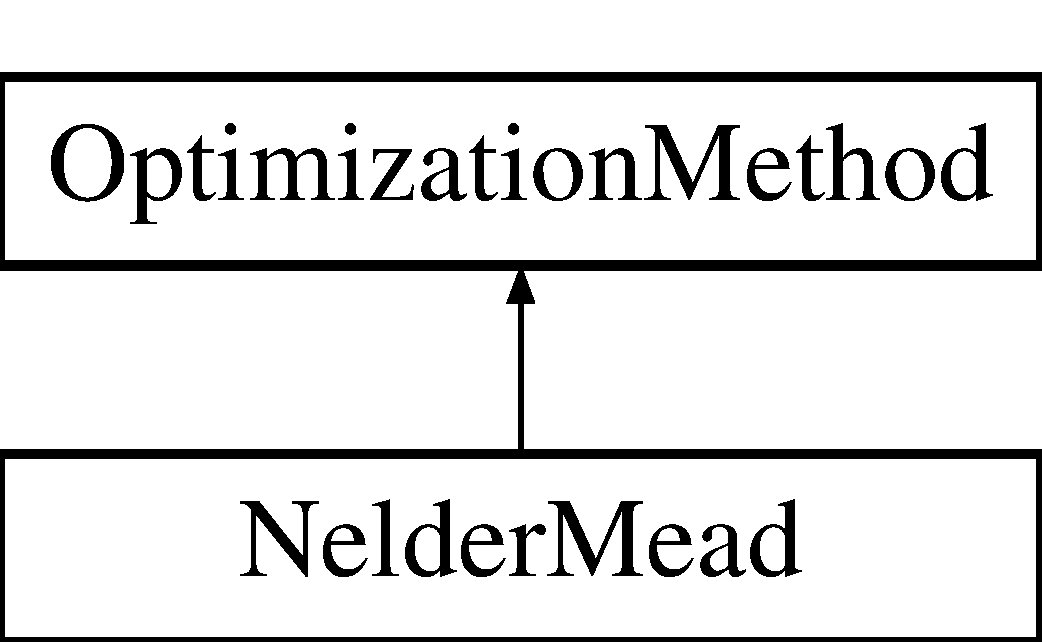
\includegraphics[height=2.000000cm]{class_nelder_mead}
\end{center}
\end{figure}
\subsection*{Public Member Functions}
\begin{DoxyCompactItemize}
\item 
\hyperlink{class_nelder_mead_afbf2f00242cc95bd533c8bd6a5dfbba6}{Nelder\+Mead} (double \+\_\+reflection=1.\+0, double \+\_\+expansion=2.\+0, double \+\_\+contraction=0.\+5, double \+\_\+shrink=0.\+5)
\item 
\mbox{\Hypertarget{class_nelder_mead_a0b52b4a63babb9a1849c51de1445947c}\label{class_nelder_mead_a0b52b4a63babb9a1849c51de1445947c}} 
virtual \hyperlink{class_nelder_mead_a0b52b4a63babb9a1849c51de1445947c}{$\sim$\+Nelder\+Mead} ()
\begin{DoxyCompactList}\small\item\em destructor \end{DoxyCompactList}\item 
virtual \hyperlink{struct_opt_result}{Opt\+Result} \hyperlink{class_nelder_mead_a67ad06a8e8f67f6c6a28bfe2d61afd08}{Optimize} (std\+::shared\+\_\+ptr$<$ \hyperlink{class_area}{Area} $>$ A, std\+::shared\+\_\+ptr$<$ \hyperlink{class_function}{Function} $>$ F, std\+::shared\+\_\+ptr$<$ \hyperlink{class_terminal_condition}{Terminal\+Condition} $>$ T, const \hyperlink{classv_point}{v\+Point} \&First\+Point)
\item 
\mbox{\Hypertarget{class_nelder_mead_a54134743c71c8790210b1249c577505e}\label{class_nelder_mead_a54134743c71c8790210b1249c577505e}} 
virtual char $\ast$ \hyperlink{class_nelder_mead_a54134743c71c8790210b1249c577505e}{Name} () const
\begin{DoxyCompactList}\small\item\em returns the name of the method \end{DoxyCompactList}\item 
\mbox{\Hypertarget{class_nelder_mead_aa8844aa9b710ab1e611a071e8a2ef282}\label{class_nelder_mead_aa8844aa9b710ab1e611a071e8a2ef282}} 
bool \hyperlink{class_nelder_mead_aa8844aa9b710ab1e611a071e8a2ef282}{Set\+Reflection} (double \+\_\+reflection)
\begin{DoxyCompactList}\small\item\em sets the reflection parameter of the method with argument validation \end{DoxyCompactList}\item 
\mbox{\Hypertarget{class_nelder_mead_a07345c18aa9b15bf061b7b040cb1c485}\label{class_nelder_mead_a07345c18aa9b15bf061b7b040cb1c485}} 
bool \hyperlink{class_nelder_mead_a07345c18aa9b15bf061b7b040cb1c485}{Set\+Expansion} (double \+\_\+expansion)
\begin{DoxyCompactList}\small\item\em sets the expansion parameter of the method with argument validation \end{DoxyCompactList}\item 
\mbox{\Hypertarget{class_nelder_mead_a1ecc71f01ee28a75efa27addb041670e}\label{class_nelder_mead_a1ecc71f01ee28a75efa27addb041670e}} 
bool \hyperlink{class_nelder_mead_a1ecc71f01ee28a75efa27addb041670e}{Set\+Contraction} (double \+\_\+contraction)
\begin{DoxyCompactList}\small\item\em sets the contraction parameter of the method with argument validation \end{DoxyCompactList}\item 
\mbox{\Hypertarget{class_nelder_mead_a93d6e7b0cc0fdec157a7975c52c2da80}\label{class_nelder_mead_a93d6e7b0cc0fdec157a7975c52c2da80}} 
bool \hyperlink{class_nelder_mead_a93d6e7b0cc0fdec157a7975c52c2da80}{Set\+Shrink} (double \+\_\+shrink)
\begin{DoxyCompactList}\small\item\em sets the shrink parameter of the method with argument validation \end{DoxyCompactList}\item 
\mbox{\Hypertarget{class_nelder_mead_a8ef919184e1d3da6c126d1edf56162b2}\label{class_nelder_mead_a8ef919184e1d3da6c126d1edf56162b2}} 
double \hyperlink{class_nelder_mead_a8ef919184e1d3da6c126d1edf56162b2}{Get\+Reflection} () const
\begin{DoxyCompactList}\small\item\em returns the reflection parameter of the method \end{DoxyCompactList}\item 
\mbox{\Hypertarget{class_nelder_mead_a819eb62e9a97129acb690753ddae7c0f}\label{class_nelder_mead_a819eb62e9a97129acb690753ddae7c0f}} 
double \hyperlink{class_nelder_mead_a819eb62e9a97129acb690753ddae7c0f}{Get\+Expansion} () const
\begin{DoxyCompactList}\small\item\em returns the expansion parameter of the method \end{DoxyCompactList}\item 
\mbox{\Hypertarget{class_nelder_mead_a1b370090db3d9b58a662eab50a6ed3c9}\label{class_nelder_mead_a1b370090db3d9b58a662eab50a6ed3c9}} 
double \hyperlink{class_nelder_mead_a1b370090db3d9b58a662eab50a6ed3c9}{Get\+Contraction} () const
\begin{DoxyCompactList}\small\item\em returns the contraction parameter of the method \end{DoxyCompactList}\item 
\mbox{\Hypertarget{class_nelder_mead_a2333e386995f2a3025ec61a20c5d3f0f}\label{class_nelder_mead_a2333e386995f2a3025ec61a20c5d3f0f}} 
double \hyperlink{class_nelder_mead_a2333e386995f2a3025ec61a20c5d3f0f}{Get\+Shrink} () const
\begin{DoxyCompactList}\small\item\em returns the shrink parameter of the method \end{DoxyCompactList}\item 
\mbox{\Hypertarget{class_nelder_mead_a651153fd9c477da6e2aeeb2473251506}\label{class_nelder_mead_a651153fd9c477da6e2aeeb2473251506}} 
virtual void \hyperlink{class_nelder_mead_a651153fd9c477da6e2aeeb2473251506}{Info} () const
\begin{DoxyCompactList}\small\item\em writes the information about the method and its arguments to std\+::cout \end{DoxyCompactList}\end{DoxyCompactItemize}


\subsection{Detailed Description}
\hypertarget{function_8h_DESCRIPTION}{}\subsection{D\+E\+S\+C\+R\+I\+P\+T\+I\+ON}\label{function_8h_DESCRIPTION}
The \hyperlink{class_nelder_mead}{Nelder\+Mead} class is derived from \hyperlink{class_optimization_method}{Optimization\+Method} and represents an instance of Nelder-\/\+Mead optimization algorithm with algorithm parameters 

\subsection{Constructor \& Destructor Documentation}
\mbox{\Hypertarget{class_nelder_mead_afbf2f00242cc95bd533c8bd6a5dfbba6}\label{class_nelder_mead_afbf2f00242cc95bd533c8bd6a5dfbba6}} 
\index{Nelder\+Mead@{Nelder\+Mead}!Nelder\+Mead@{Nelder\+Mead}}
\index{Nelder\+Mead@{Nelder\+Mead}!Nelder\+Mead@{Nelder\+Mead}}
\subsubsection{\texorpdfstring{Nelder\+Mead()}{NelderMead()}}
{\footnotesize\ttfamily Nelder\+Mead\+::\+Nelder\+Mead (\begin{DoxyParamCaption}\item[{double}]{\+\_\+reflection = {\ttfamily 1.0},  }\item[{double}]{\+\_\+expansion = {\ttfamily 2.0},  }\item[{double}]{\+\_\+contraction = {\ttfamily 0.5},  }\item[{double}]{\+\_\+shrink = {\ttfamily 0.5} }\end{DoxyParamCaption})}

constructor that sets the parameters of the method to the given values or to default values if no value is provided 

\subsection{Member Function Documentation}
\mbox{\Hypertarget{class_nelder_mead_a67ad06a8e8f67f6c6a28bfe2d61afd08}\label{class_nelder_mead_a67ad06a8e8f67f6c6a28bfe2d61afd08}} 
\index{Nelder\+Mead@{Nelder\+Mead}!Optimize@{Optimize}}
\index{Optimize@{Optimize}!Nelder\+Mead@{Nelder\+Mead}}
\subsubsection{\texorpdfstring{Optimize()}{Optimize()}}
{\footnotesize\ttfamily \hyperlink{struct_opt_result}{Opt\+Result} Nelder\+Mead\+::\+Optimize (\begin{DoxyParamCaption}\item[{std\+::shared\+\_\+ptr$<$ \hyperlink{class_area}{Area} $>$}]{A,  }\item[{std\+::shared\+\_\+ptr$<$ \hyperlink{class_function}{Function} $>$}]{F,  }\item[{std\+::shared\+\_\+ptr$<$ \hyperlink{class_terminal_condition}{Terminal\+Condition} $>$}]{T,  }\item[{const \hyperlink{classv_point}{v\+Point} \&}]{First\+Point }\end{DoxyParamCaption})\hspace{0.3cm}{\ttfamily [virtual]}}

inherited from \hyperlink{class_optimization_method}{Optimization\+Method} optimizes the function in given area using the Nelder-\/\+Mead algorithm 

Implements \hyperlink{class_optimization_method_a98a1e917667c3ca851cbcd9068b0a9d9}{Optimization\+Method}.



The documentation for this class was generated from the following files\+:\begin{DoxyCompactItemize}
\item 
nelder\+\_\+mead.\+h\item 
nelder\+\_\+mead.\+cpp\end{DoxyCompactItemize}

\hypertarget{class_optimization_method}{}\section{Optimization\+Method Class Reference}
\label{class_optimization_method}\index{Optimization\+Method@{Optimization\+Method}}


{\ttfamily \#include $<$optimization\+\_\+method.\+h$>$}

Inheritance diagram for Optimization\+Method\+:\begin{figure}[H]
\begin{center}
\leavevmode
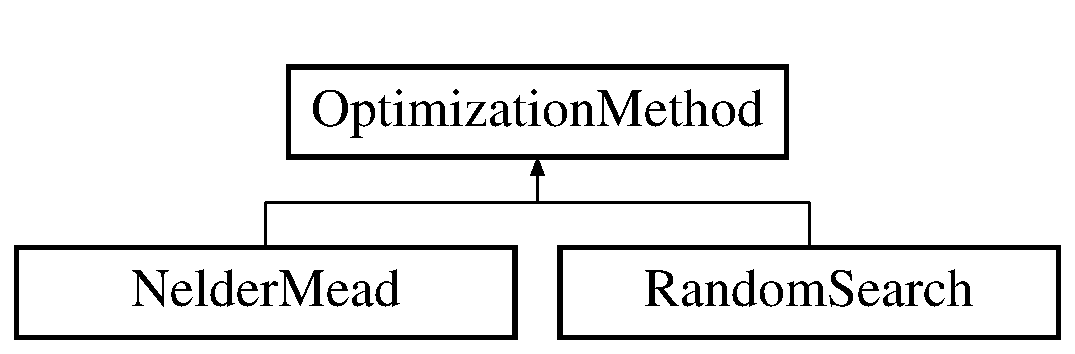
\includegraphics[height=2.000000cm]{class_optimization_method}
\end{center}
\end{figure}
\subsection*{Public Member Functions}
\begin{DoxyCompactItemize}
\item 
\mbox{\Hypertarget{class_optimization_method_a8490a7cd0e3334f7e61469377c7d4217}\label{class_optimization_method_a8490a7cd0e3334f7e61469377c7d4217}} 
\hyperlink{class_optimization_method_a8490a7cd0e3334f7e61469377c7d4217}{Optimization\+Method} ()
\begin{DoxyCompactList}\small\item\em constructor \end{DoxyCompactList}\item 
\mbox{\Hypertarget{class_optimization_method_ab33ddd12499ebedbc73f125a65a21442}\label{class_optimization_method_ab33ddd12499ebedbc73f125a65a21442}} 
virtual \hyperlink{class_optimization_method_ab33ddd12499ebedbc73f125a65a21442}{$\sim$\+Optimization\+Method} ()
\begin{DoxyCompactList}\small\item\em destructor \end{DoxyCompactList}\item 
virtual \hyperlink{struct_opt_result}{Opt\+Result} \hyperlink{class_optimization_method_a98a1e917667c3ca851cbcd9068b0a9d9}{Optimize} (std\+::shared\+\_\+ptr$<$ \hyperlink{class_area}{Area} $>$ A, std\+::shared\+\_\+ptr$<$ \hyperlink{class_function}{Function} $>$ F, std\+::shared\+\_\+ptr$<$ \hyperlink{class_terminal_condition}{Terminal\+Condition} $>$ T, const \hyperlink{classv_point}{v\+Point} \&First\+Point)=0
\item 
\mbox{\Hypertarget{class_optimization_method_a2bb0f33d599675937787db8bd17197c1}\label{class_optimization_method_a2bb0f33d599675937787db8bd17197c1}} 
virtual char $\ast$ \hyperlink{class_optimization_method_a2bb0f33d599675937787db8bd17197c1}{Name} () const =0
\begin{DoxyCompactList}\small\item\em abstract method that returns the name of the method \end{DoxyCompactList}\item 
\mbox{\Hypertarget{class_optimization_method_adc3fa59ab209fd11044696319b45cf2a}\label{class_optimization_method_adc3fa59ab209fd11044696319b45cf2a}} 
virtual void \hyperlink{class_optimization_method_adc3fa59ab209fd11044696319b45cf2a}{Info} () const =0
\begin{DoxyCompactList}\small\item\em abstract method that writes the information about the method to std\+::cout \end{DoxyCompactList}\end{DoxyCompactItemize}
\subsection*{Friends}
\begin{DoxyCompactItemize}
\item 
std\+::ostream \& \hyperlink{class_optimization_method_ad4282eaeda272e5bec7a542d1889253a}{operator$<$$<$} (std\+::ostream \&out, std\+::shared\+\_\+ptr$<$ \hyperlink{class_optimization_method}{Optimization\+Method} $>$ opt\+Method)
\end{DoxyCompactItemize}


\subsection{Detailed Description}
\hypertarget{function_8h_DESCRIPTION}{}\subsection{D\+E\+S\+C\+R\+I\+P\+T\+I\+ON}\label{function_8h_DESCRIPTION}
The \hyperlink{class_optimization_method}{Optimization\+Method} class represent an optimization method with the method parameters 

\subsection{Member Function Documentation}
\mbox{\Hypertarget{class_optimization_method_a98a1e917667c3ca851cbcd9068b0a9d9}\label{class_optimization_method_a98a1e917667c3ca851cbcd9068b0a9d9}} 
\index{Optimization\+Method@{Optimization\+Method}!Optimize@{Optimize}}
\index{Optimize@{Optimize}!Optimization\+Method@{Optimization\+Method}}
\subsubsection{\texorpdfstring{Optimize()}{Optimize()}}
{\footnotesize\ttfamily virtual \hyperlink{struct_opt_result}{Opt\+Result} Optimization\+Method\+::\+Optimize (\begin{DoxyParamCaption}\item[{std\+::shared\+\_\+ptr$<$ \hyperlink{class_area}{Area} $>$}]{A,  }\item[{std\+::shared\+\_\+ptr$<$ \hyperlink{class_function}{Function} $>$}]{F,  }\item[{std\+::shared\+\_\+ptr$<$ \hyperlink{class_terminal_condition}{Terminal\+Condition} $>$}]{T,  }\item[{const \hyperlink{classv_point}{v\+Point} \&}]{First\+Point }\end{DoxyParamCaption})\hspace{0.3cm}{\ttfamily [pure virtual]}}

abstract method that runs the optimization process using the optimization method for a function in given area with given terminal condition 
\begin{DoxyParams}{Parameters}
{\em A} & pointer the area in which the function is optimized \\
\hline
{\em F} & pointer to the function that is optimized \\
\hline
{\em T} & pointer to the terminal condition for the method \\
\hline
{\em First\+Point} & vector point from which the optimization process begins \\
\hline
\end{DoxyParams}
\begin{DoxyReturn}{Returns}
\hyperlink{struct_opt_result}{Opt\+Result} structure with the result of the optimization 
\end{DoxyReturn}


Implemented in \hyperlink{class_random_search_a869069d90b1c12ec67182f415be7e8ce}{Random\+Search}, and \hyperlink{class_nelder_mead_a67ad06a8e8f67f6c6a28bfe2d61afd08}{Nelder\+Mead}.



\subsection{Friends And Related Function Documentation}
\mbox{\Hypertarget{class_optimization_method_ad4282eaeda272e5bec7a542d1889253a}\label{class_optimization_method_ad4282eaeda272e5bec7a542d1889253a}} 
\index{Optimization\+Method@{Optimization\+Method}!operator$<$$<$@{operator$<$$<$}}
\index{operator$<$$<$@{operator$<$$<$}!Optimization\+Method@{Optimization\+Method}}
\subsubsection{\texorpdfstring{operator$<$$<$}{operator<<}}
{\footnotesize\ttfamily std\+::ostream\& operator$<$$<$ (\begin{DoxyParamCaption}\item[{std\+::ostream \&}]{out,  }\item[{std\+::shared\+\_\+ptr$<$ \hyperlink{class_optimization_method}{Optimization\+Method} $>$}]{opt\+Method }\end{DoxyParamCaption})\hspace{0.3cm}{\ttfamily [friend]}}

overloaded output operator for std\+::cout 

The documentation for this class was generated from the following file\+:\begin{DoxyCompactItemize}
\item 
optimization\+\_\+method.\+h\end{DoxyCompactItemize}

\hypertarget{struct_opt_result}{}\section{Opt\+Result Struct Reference}
\label{struct_opt_result}\index{Opt\+Result@{Opt\+Result}}


{\ttfamily \#include $<$optimization\+\_\+method.\+h$>$}

\subsection*{Public Attributes}
\begin{DoxyCompactItemize}
\item 
\mbox{\Hypertarget{struct_opt_result_ac00c99bd944240cc974270276330a9a0}\label{struct_opt_result_ac00c99bd944240cc974270276330a9a0}} 
std\+::shared\+\_\+ptr$<$ \hyperlink{class_function}{Function} $>$ \hyperlink{struct_opt_result_ac00c99bd944240cc974270276330a9a0}{Fun}
\begin{DoxyCompactList}\small\item\em pointer to the function for which the optimization was done \end{DoxyCompactList}\item 
\mbox{\Hypertarget{struct_opt_result_a6edfe9aa97b9b9f878d5608cde3708a3}\label{struct_opt_result_a6edfe9aa97b9b9f878d5608cde3708a3}} 
std\+::shared\+\_\+ptr$<$ \hyperlink{class_area}{Area} $>$ \hyperlink{struct_opt_result_a6edfe9aa97b9b9f878d5608cde3708a3}{Opt\+Area}
\begin{DoxyCompactList}\small\item\em pointer to the area in which the optimization was done \end{DoxyCompactList}\item 
\mbox{\Hypertarget{struct_opt_result_ad461a01a3be3bdce6b78713f701342c9}\label{struct_opt_result_ad461a01a3be3bdce6b78713f701342c9}} 
std\+::vector$<$ \hyperlink{classv_point}{v\+Point} $>$ \hyperlink{struct_opt_result_ad461a01a3be3bdce6b78713f701342c9}{Approximations}
\begin{DoxyCompactList}\small\item\em std\+::vector of approximation vector points \end{DoxyCompactList}\item 
\mbox{\Hypertarget{struct_opt_result_a0ba90701207d29e434638eac26f0d446}\label{struct_opt_result_a0ba90701207d29e434638eac26f0d446}} 
std\+::vector$<$ double $>$ \hyperlink{struct_opt_result_a0ba90701207d29e434638eac26f0d446}{Evaluations}
\begin{DoxyCompactList}\small\item\em std\+::vector of function evaluations in approximation points \end{DoxyCompactList}\item 
\mbox{\Hypertarget{struct_opt_result_ac4a11d14ca2867cff055e94ea49082cb}\label{struct_opt_result_ac4a11d14ca2867cff055e94ea49082cb}} 
\hyperlink{classv_point}{v\+Point} \hyperlink{struct_opt_result_ac4a11d14ca2867cff055e94ea49082cb}{Result}
\begin{DoxyCompactList}\small\item\em vector point that represents the result of optimization \end{DoxyCompactList}\item 
\mbox{\Hypertarget{struct_opt_result_ac2f40006e97cd3b32b8d36cb61e8c9b5}\label{struct_opt_result_ac2f40006e97cd3b32b8d36cb61e8c9b5}} 
double \hyperlink{struct_opt_result_ac2f40006e97cd3b32b8d36cb61e8c9b5}{Res\+Func\+Value}
\begin{DoxyCompactList}\small\item\em function evaluation value in the resulting point \end{DoxyCompactList}\item 
\mbox{\Hypertarget{struct_opt_result_a66494a483f7a183f8c382fa13e445b33}\label{struct_opt_result_a66494a483f7a183f8c382fa13e445b33}} 
int \hyperlink{struct_opt_result_a66494a483f7a183f8c382fa13e445b33}{Iterations}
\begin{DoxyCompactList}\small\item\em number of iterations of the optimization process \end{DoxyCompactList}\end{DoxyCompactItemize}


\subsection{Detailed Description}
\hypertarget{function_8h_DESCRIPTION}{}\subsection{D\+E\+S\+C\+R\+I\+P\+T\+I\+ON}\label{function_8h_DESCRIPTION}
The \hyperlink{struct_opt_result}{Opt\+Result} structure represents the result of optimization process for a function in given area 

The documentation for this struct was generated from the following file\+:\begin{DoxyCompactItemize}
\item 
optimization\+\_\+method.\+h\end{DoxyCompactItemize}

\hypertarget{class_random_search}{}\section{Random\+Search Class Reference}
\label{class_random_search}\index{Random\+Search@{Random\+Search}}


{\ttfamily \#include $<$random\+\_\+search.\+h$>$}

Inheritance diagram for Random\+Search\+:\begin{figure}[H]
\begin{center}
\leavevmode
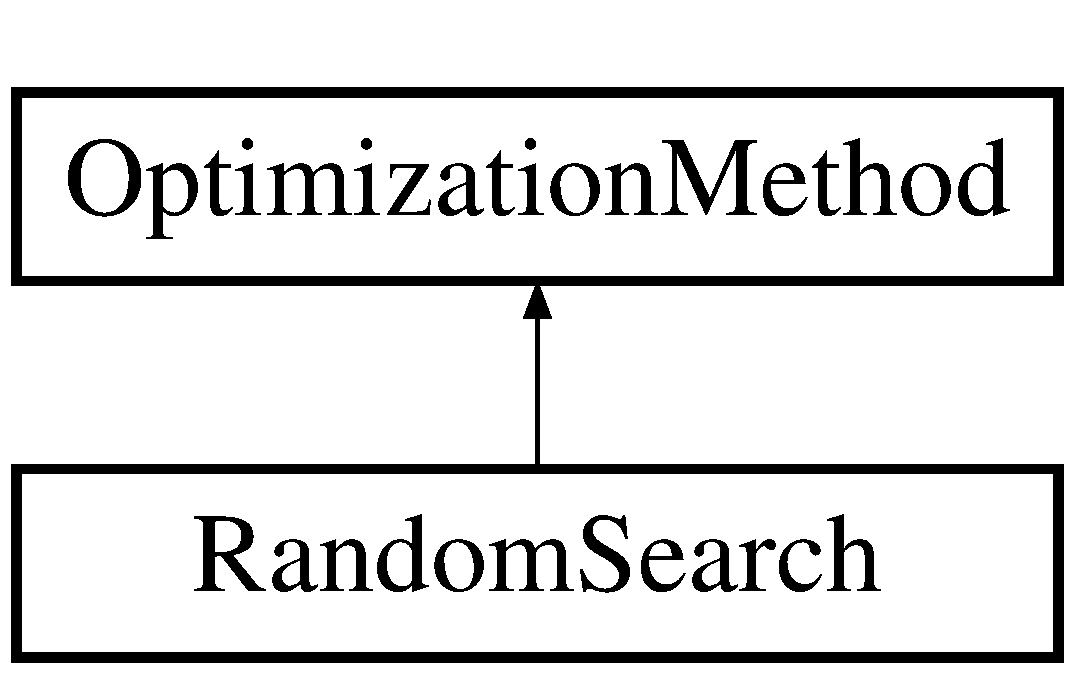
\includegraphics[height=2.000000cm]{class_random_search}
\end{center}
\end{figure}
\subsection*{Public Member Functions}
\begin{DoxyCompactItemize}
\item 
\hyperlink{class_random_search_a92e55b6d0dee76ebbae1c03685c25499}{Random\+Search} (double \+\_\+p=0.\+5, double \+\_\+gamma=0.\+5)
\item 
\mbox{\Hypertarget{class_random_search_a32308c3507abcf02bc0f7da0c53b5ab6}\label{class_random_search_a32308c3507abcf02bc0f7da0c53b5ab6}} 
double {\bfseries GetP} () const
\item 
double \hyperlink{class_random_search_a4009e36c2e604791a3f050280262fcc6}{Get\+Gamma} () const
\begin{DoxyCompactList}\small\item\em returns the bernoulli distribution parameter of the method \end{DoxyCompactList}\item 
\mbox{\Hypertarget{class_random_search_a1aef08ec9c0eb451d0c3350c99285506}\label{class_random_search_a1aef08ec9c0eb451d0c3350c99285506}} 
bool \hyperlink{class_random_search_a1aef08ec9c0eb451d0c3350c99285506}{SetP} (double \+\_\+p)
\begin{DoxyCompactList}\small\item\em sets the bernoulli distribution parameter of the method with argument validation \end{DoxyCompactList}\item 
\mbox{\Hypertarget{class_random_search_ad092544a0368d64432128842c365ed44}\label{class_random_search_ad092544a0368d64432128842c365ed44}} 
bool \hyperlink{class_random_search_ad092544a0368d64432128842c365ed44}{Set\+Gamma} (double \+\_\+gamma)
\begin{DoxyCompactList}\small\item\em sets the shrinking parameter of the method with argument validation \end{DoxyCompactList}\item 
virtual \hyperlink{struct_opt_result}{Opt\+Result} \hyperlink{class_random_search_a869069d90b1c12ec67182f415be7e8ce}{Optimize} (std\+::shared\+\_\+ptr$<$ \hyperlink{class_area}{Area} $>$ A, std\+::shared\+\_\+ptr$<$ \hyperlink{class_function}{Function} $>$ F, std\+::shared\+\_\+ptr$<$ \hyperlink{class_terminal_condition}{Terminal\+Condition} $>$ T, const \hyperlink{classv_point}{v\+Point} \&First\+Point)
\item 
\mbox{\Hypertarget{class_random_search_a3fcfd10ed0c2227c0bd7647e1a9be403}\label{class_random_search_a3fcfd10ed0c2227c0bd7647e1a9be403}} 
virtual char $\ast$ \hyperlink{class_random_search_a3fcfd10ed0c2227c0bd7647e1a9be403}{Name} () const
\begin{DoxyCompactList}\small\item\em returns the name of the method \end{DoxyCompactList}\item 
\mbox{\Hypertarget{class_random_search_a3229882f90a1a956d204447bd76781a4}\label{class_random_search_a3229882f90a1a956d204447bd76781a4}} 
virtual void \hyperlink{class_random_search_a3229882f90a1a956d204447bd76781a4}{Info} () const
\begin{DoxyCompactList}\small\item\em writes the information about the method and its arguments to std\+::cout \end{DoxyCompactList}\end{DoxyCompactItemize}


\subsection{Detailed Description}
\hypertarget{function_8h_DESCRIPTION}{}\subsection{D\+E\+S\+C\+R\+I\+P\+T\+I\+ON}\label{function_8h_DESCRIPTION}
The \hyperlink{class_nelder_mead}{Nelder\+Mead} class is derived from \hyperlink{class_optimization_method}{Optimization\+Method} and represents an instance of Nelder-\/\+Mead optimization algorithm with algorithm parameters 

\subsection{Constructor \& Destructor Documentation}
\mbox{\Hypertarget{class_random_search_a92e55b6d0dee76ebbae1c03685c25499}\label{class_random_search_a92e55b6d0dee76ebbae1c03685c25499}} 
\index{Random\+Search@{Random\+Search}!Random\+Search@{Random\+Search}}
\index{Random\+Search@{Random\+Search}!Random\+Search@{Random\+Search}}
\subsubsection{\texorpdfstring{Random\+Search()}{RandomSearch()}}
{\footnotesize\ttfamily Random\+Search\+::\+Random\+Search (\begin{DoxyParamCaption}\item[{double}]{\+\_\+p = {\ttfamily 0.5},  }\item[{double}]{\+\_\+gamma = {\ttfamily 0.5} }\end{DoxyParamCaption})\hspace{0.3cm}{\ttfamily [inline]}}

constructor that sets the parameters of the method to the given values or to default values if no value is provided 

\subsection{Member Function Documentation}
\mbox{\Hypertarget{class_random_search_a4009e36c2e604791a3f050280262fcc6}\label{class_random_search_a4009e36c2e604791a3f050280262fcc6}} 
\index{Random\+Search@{Random\+Search}!Get\+Gamma@{Get\+Gamma}}
\index{Get\+Gamma@{Get\+Gamma}!Random\+Search@{Random\+Search}}
\subsubsection{\texorpdfstring{Get\+Gamma()}{GetGamma()}}
{\footnotesize\ttfamily double Random\+Search\+::\+Get\+Gamma (\begin{DoxyParamCaption}{ }\end{DoxyParamCaption}) const\hspace{0.3cm}{\ttfamily [inline]}}



returns the bernoulli distribution parameter of the method 

returns the shrinking parameter of the method \mbox{\Hypertarget{class_random_search_a869069d90b1c12ec67182f415be7e8ce}\label{class_random_search_a869069d90b1c12ec67182f415be7e8ce}} 
\index{Random\+Search@{Random\+Search}!Optimize@{Optimize}}
\index{Optimize@{Optimize}!Random\+Search@{Random\+Search}}
\subsubsection{\texorpdfstring{Optimize()}{Optimize()}}
{\footnotesize\ttfamily \hyperlink{struct_opt_result}{Opt\+Result} Random\+Search\+::\+Optimize (\begin{DoxyParamCaption}\item[{std\+::shared\+\_\+ptr$<$ \hyperlink{class_area}{Area} $>$}]{A,  }\item[{std\+::shared\+\_\+ptr$<$ \hyperlink{class_function}{Function} $>$}]{F,  }\item[{std\+::shared\+\_\+ptr$<$ \hyperlink{class_terminal_condition}{Terminal\+Condition} $>$}]{T,  }\item[{const \hyperlink{classv_point}{v\+Point} \&}]{First\+Point }\end{DoxyParamCaption})\hspace{0.3cm}{\ttfamily [virtual]}}

inherited from \hyperlink{class_optimization_method}{Optimization\+Method} optimizes the function in given area using the modified Random Search algorithm 

Implements \hyperlink{class_optimization_method_a98a1e917667c3ca851cbcd9068b0a9d9}{Optimization\+Method}.



The documentation for this class was generated from the following files\+:\begin{DoxyCompactItemize}
\item 
random\+\_\+search.\+h\item 
random\+\_\+search.\+cpp\end{DoxyCompactItemize}

\hypertarget{class_range}{}\section{Range Class Reference}
\label{class_range}\index{Range@{Range}}


{\ttfamily \#include $<$range.\+h$>$}

Inheritance diagram for Range\+:\begin{figure}[H]
\begin{center}
\leavevmode
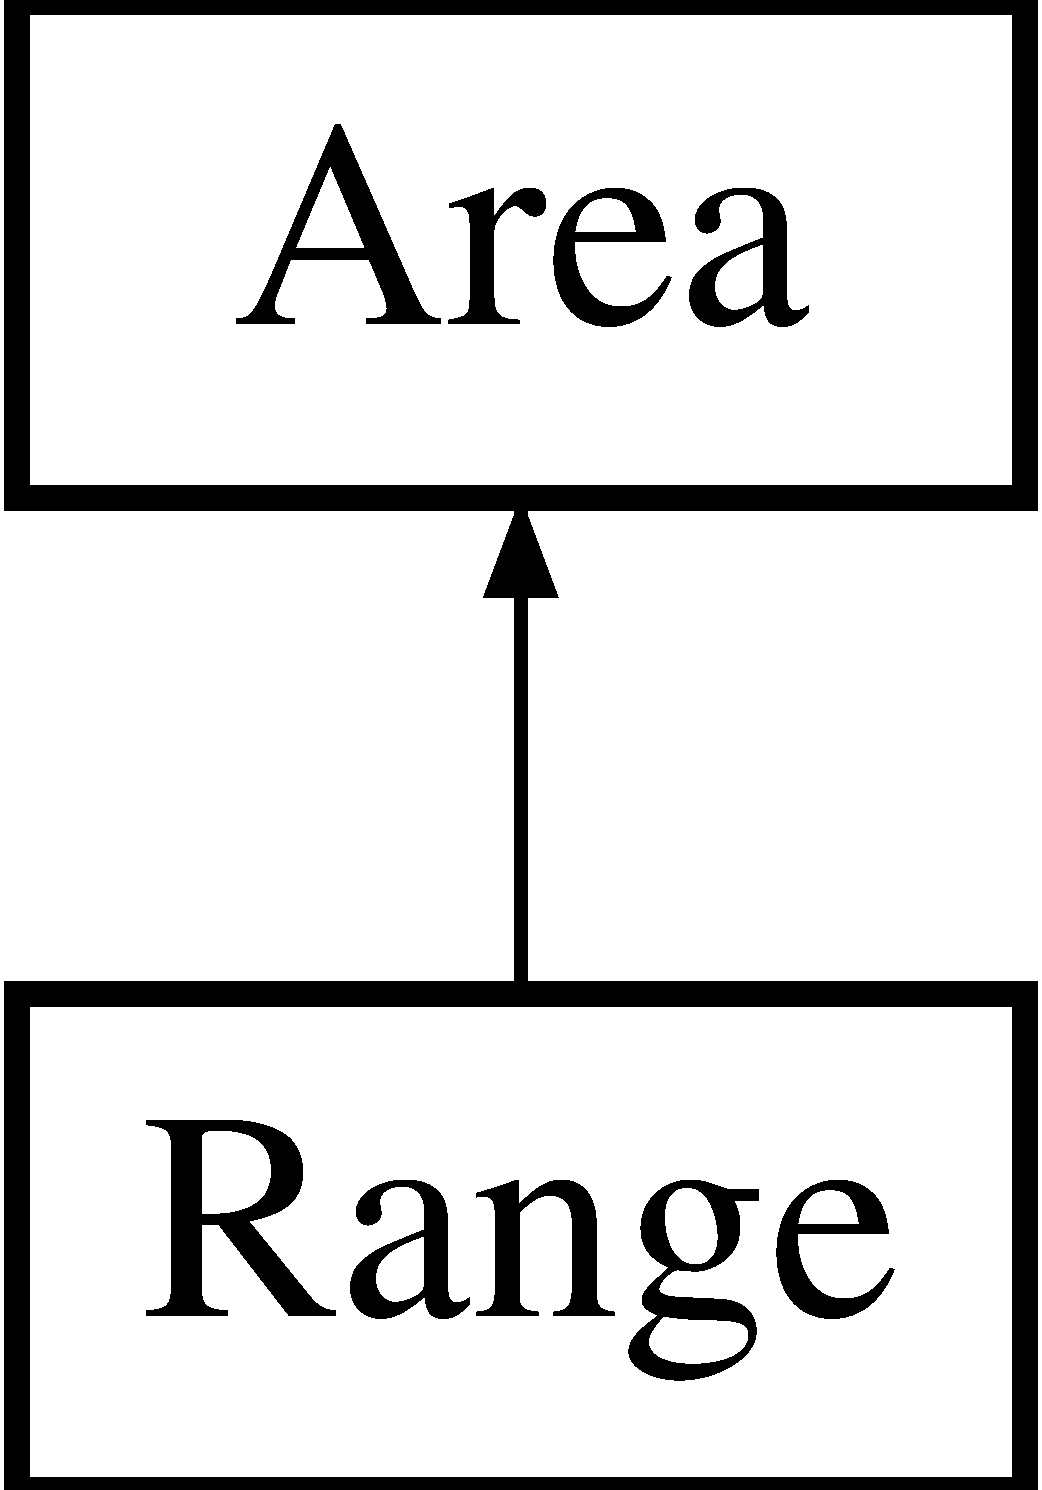
\includegraphics[height=2.000000cm]{class_range}
\end{center}
\end{figure}
\subsection*{Public Member Functions}
\begin{DoxyCompactItemize}
\item 
\hyperlink{class_range_aad92f98f8860648f7d6756f0c07d66ba}{Range} (double \+\_\+min=-\/1.\+0, double \+\_\+max=1.\+0)
\item 
\mbox{\Hypertarget{class_range_a55756d815e35f6a003536342cf2e694b}\label{class_range_a55756d815e35f6a003536342cf2e694b}} 
virtual \hyperlink{class_range_a55756d815e35f6a003536342cf2e694b}{$\sim$\+Range} ()
\begin{DoxyCompactList}\small\item\em destructor \end{DoxyCompactList}\item 
virtual bool \hyperlink{class_range_abaec0363220c4fbedaca148a4790bc9e}{In} (const \hyperlink{classv_point}{v\+Point} \&X) const
\item 
bool \hyperlink{class_range_a2d76a15c78b08d8c14dd076b630ee1eb}{In} (double X) const
\begin{DoxyCompactList}\small\item\em checks whether a double number is within the range \end{DoxyCompactList}\item 
virtual \hyperlink{classv_point}{v\+Point} \hyperlink{class_range_a71795faae3f99507eb999e7df0c248da}{Random\+Point} () const
\item 
virtual std\+::shared\+\_\+ptr$<$ \hyperlink{class_area}{Area} $>$ \hyperlink{class_range_ab75514ad9a6e950a15d901020a65119a}{Sub\+Area} (const \hyperlink{classv_point}{v\+Point} \&X, double epsilon) const
\item 
\mbox{\Hypertarget{class_range_afd09ccc714abb96009efd345ee2b8f91}\label{class_range_afd09ccc714abb96009efd345ee2b8f91}} 
double \hyperlink{class_range_afd09ccc714abb96009efd345ee2b8f91}{Get\+Max} () const
\begin{DoxyCompactList}\small\item\em return the right bound of the range \end{DoxyCompactList}\item 
\mbox{\Hypertarget{class_range_ad1a4ac0512e07c9987c9b78297e9ae4e}\label{class_range_ad1a4ac0512e07c9987c9b78297e9ae4e}} 
double \hyperlink{class_range_ad1a4ac0512e07c9987c9b78297e9ae4e}{Get\+Min} () const
\begin{DoxyCompactList}\small\item\em return the left bound of the range \end{DoxyCompactList}\item 
virtual void \hyperlink{class_range_adcbfaa8ea3d2e6da005573fd8146e952}{Info} () const
\end{DoxyCompactItemize}
\subsection*{Friends}
\begin{DoxyCompactItemize}
\item 
std\+::ostream \& \hyperlink{class_range_a4720a1c61f7e023f4ae120b4eeb5a1da}{operator$<$$<$} (std\+::ostream \&out, std\+::shared\+\_\+ptr$<$ \hyperlink{class_range}{Range} $>$ R)
\end{DoxyCompactItemize}
\subsection*{Additional Inherited Members}


\subsection{Detailed Description}
\hypertarget{function_8h_DESCRIPTION}{}\subsection{D\+E\+S\+C\+R\+I\+P\+T\+I\+ON}\label{function_8h_DESCRIPTION}
The \hyperlink{class_range}{Range} class is derived from \hyperlink{class_area}{Area} and represents a onedimensional range of real numbers (a, b) 

\subsection{Constructor \& Destructor Documentation}
\mbox{\Hypertarget{class_range_aad92f98f8860648f7d6756f0c07d66ba}\label{class_range_aad92f98f8860648f7d6756f0c07d66ba}} 
\index{Range@{Range}!Range@{Range}}
\index{Range@{Range}!Range@{Range}}
\subsubsection{\texorpdfstring{Range()}{Range()}}
{\footnotesize\ttfamily Range\+::\+Range (\begin{DoxyParamCaption}\item[{double}]{\+\_\+min = {\ttfamily -\/1.0},  }\item[{double}]{\+\_\+max = {\ttfamily 1.0} }\end{DoxyParamCaption})\hspace{0.3cm}{\ttfamily [inline]}}

constructor that sets the bounds of the range 

\subsection{Member Function Documentation}
\mbox{\Hypertarget{class_range_abaec0363220c4fbedaca148a4790bc9e}\label{class_range_abaec0363220c4fbedaca148a4790bc9e}} 
\index{Range@{Range}!In@{In}}
\index{In@{In}!Range@{Range}}
\subsubsection{\texorpdfstring{In()}{In()}\hspace{0.1cm}{\footnotesize\ttfamily [1/2]}}
{\footnotesize\ttfamily virtual bool Range\+::\+In (\begin{DoxyParamCaption}\item[{const \hyperlink{classv_point}{v\+Point} \&}]{X }\end{DoxyParamCaption}) const\hspace{0.3cm}{\ttfamily [inline]}, {\ttfamily [virtual]}}

inhereted from \hyperlink{class_area}{Area} 
\begin{DoxyParams}{Parameters}
{\em X} & vector point \\
\hline
\end{DoxyParams}
\begin{DoxyReturn}{Returns}
true if X is onedimensional and its coordinate is in the range and false otherwise 
\end{DoxyReturn}


Implements \hyperlink{class_area_a08775973fcf205fb91654b25a08f6bea}{Area}.

\mbox{\Hypertarget{class_range_a2d76a15c78b08d8c14dd076b630ee1eb}\label{class_range_a2d76a15c78b08d8c14dd076b630ee1eb}} 
\index{Range@{Range}!In@{In}}
\index{In@{In}!Range@{Range}}
\subsubsection{\texorpdfstring{In()}{In()}\hspace{0.1cm}{\footnotesize\ttfamily [2/2]}}
{\footnotesize\ttfamily bool Range\+::\+In (\begin{DoxyParamCaption}\item[{double}]{X }\end{DoxyParamCaption}) const\hspace{0.3cm}{\ttfamily [inline]}}



checks whether a double number is within the range 

inhereted from \hyperlink{class_area}{Area} 
\begin{DoxyParams}{Parameters}
{\em X} & vector point \\
\hline
\end{DoxyParams}
\begin{DoxyReturn}{Returns}
true if X is onedimensional and its coordinate is in the range and false otherwise 
\end{DoxyReturn}
\mbox{\Hypertarget{class_range_adcbfaa8ea3d2e6da005573fd8146e952}\label{class_range_adcbfaa8ea3d2e6da005573fd8146e952}} 
\index{Range@{Range}!Info@{Info}}
\index{Info@{Info}!Range@{Range}}
\subsubsection{\texorpdfstring{Info()}{Info()}}
{\footnotesize\ttfamily void Range\+::\+Info (\begin{DoxyParamCaption}{ }\end{DoxyParamCaption}) const\hspace{0.3cm}{\ttfamily [virtual]}}

inherited from \hyperlink{class_area}{Area} prints the range bounds to std\+::cout 

Implements \hyperlink{class_area_abc427001b3685b08cd836badffedfbbe}{Area}.

\mbox{\Hypertarget{class_range_a71795faae3f99507eb999e7df0c248da}\label{class_range_a71795faae3f99507eb999e7df0c248da}} 
\index{Range@{Range}!Random\+Point@{Random\+Point}}
\index{Random\+Point@{Random\+Point}!Range@{Range}}
\subsubsection{\texorpdfstring{Random\+Point()}{RandomPoint()}}
{\footnotesize\ttfamily \hyperlink{classv_point}{v\+Point} Range\+::\+Random\+Point (\begin{DoxyParamCaption}{ }\end{DoxyParamCaption}) const\hspace{0.3cm}{\ttfamily [virtual]}}

inhereted from \hyperlink{class_area}{Area} \begin{DoxyReturn}{Returns}
a random onedimensioal vector point uniformly distributed in the range 
\end{DoxyReturn}


Implements \hyperlink{class_area_a8a921495c0cca4095c8386f7b48ef086}{Area}.

\mbox{\Hypertarget{class_range_ab75514ad9a6e950a15d901020a65119a}\label{class_range_ab75514ad9a6e950a15d901020a65119a}} 
\index{Range@{Range}!Sub\+Area@{Sub\+Area}}
\index{Sub\+Area@{Sub\+Area}!Range@{Range}}
\subsubsection{\texorpdfstring{Sub\+Area()}{SubArea()}}
{\footnotesize\ttfamily std\+::shared\+\_\+ptr$<$ \hyperlink{class_area}{Area} $>$ Range\+::\+Sub\+Area (\begin{DoxyParamCaption}\item[{const \hyperlink{classv_point}{v\+Point} \&}]{X,  }\item[{double}]{epsilon }\end{DoxyParamCaption}) const\hspace{0.3cm}{\ttfamily [virtual]}}

inhereted from \hyperlink{class_area}{Area} \begin{DoxyReturn}{Returns}
the intersection between the epsilon range of vector point X and the range 
\end{DoxyReturn}


Implements \hyperlink{class_area_a8f28e6be12d6b1bf7217f51307ab937e}{Area}.



\subsection{Friends And Related Function Documentation}
\mbox{\Hypertarget{class_range_a4720a1c61f7e023f4ae120b4eeb5a1da}\label{class_range_a4720a1c61f7e023f4ae120b4eeb5a1da}} 
\index{Range@{Range}!operator$<$$<$@{operator$<$$<$}}
\index{operator$<$$<$@{operator$<$$<$}!Range@{Range}}
\subsubsection{\texorpdfstring{operator$<$$<$}{operator<<}}
{\footnotesize\ttfamily std\+::ostream\& operator$<$$<$ (\begin{DoxyParamCaption}\item[{std\+::ostream \&}]{out,  }\item[{std\+::shared\+\_\+ptr$<$ \hyperlink{class_range}{Range} $>$}]{R }\end{DoxyParamCaption})\hspace{0.3cm}{\ttfamily [friend]}}

prints the range bounds to std\+::cout 

The documentation for this class was generated from the following files\+:\begin{DoxyCompactItemize}
\item 
range.\+h\item 
range.\+cpp\end{DoxyCompactItemize}

\hypertarget{class_simplex}{}\section{Simplex Class Reference}
\label{class_simplex}\index{Simplex@{Simplex}}


{\ttfamily \#include $<$Simplex.\+h$>$}

\subsection*{Public Member Functions}
\begin{DoxyCompactItemize}
\item 
\mbox{\Hypertarget{class_simplex_a0556b901b7d46c7d4600aa5442f02585}\label{class_simplex_a0556b901b7d46c7d4600aa5442f02585}} 
\hyperlink{class_simplex_a0556b901b7d46c7d4600aa5442f02585}{Simplex} (int \+\_\+dim=2)
\begin{DoxyCompactList}\small\item\em creates a standard simplex with given size \end{DoxyCompactList}\item 
\mbox{\Hypertarget{class_simplex_ad227962dec843392bb95c02e106eb21c}\label{class_simplex_ad227962dec843392bb95c02e106eb21c}} 
\hyperlink{class_simplex_ad227962dec843392bb95c02e106eb21c}{Simplex} (const std\+::vector$<$ \hyperlink{classv_point}{v\+Point} $>$ \&\+\_\+vertices)
\begin{DoxyCompactList}\small\item\em creates a simplex with given vertices \end{DoxyCompactList}\item 
void \hyperlink{class_simplex_a78284170bf58df27fcd5a8df6de283f3}{Move\+To} (const \hyperlink{classv_point}{v\+Point} \&X)
\begin{DoxyCompactList}\small\item\em destructor \end{DoxyCompactList}\item 
\mbox{\Hypertarget{class_simplex_a8963be87ef81afde1c0865a71411eb1b}\label{class_simplex_a8963be87ef81afde1c0865a71411eb1b}} 
void \hyperlink{class_simplex_a8963be87ef81afde1c0865a71411eb1b}{Squeeze} (std\+::shared\+\_\+ptr$<$ \hyperlink{class_area}{Area} $>$ A)
\begin{DoxyCompactList}\small\item\em shrinks the simplex until it fits the area \end{DoxyCompactList}\item 
\mbox{\Hypertarget{class_simplex_acf5182ffe99d4420d73ac6677175587a}\label{class_simplex_acf5182ffe99d4420d73ac6677175587a}} 
const \hyperlink{classv_point}{v\+Point} \& \hyperlink{class_simplex_acf5182ffe99d4420d73ac6677175587a}{operator\mbox{[}$\,$\mbox{]}} (int index) const
\begin{DoxyCompactList}\small\item\em returns a vertex of the simplex at given index \end{DoxyCompactList}\item 
\mbox{\Hypertarget{class_simplex_a1da07de5cbb1433ea77ac92d6f68bfe7}\label{class_simplex_a1da07de5cbb1433ea77ac92d6f68bfe7}} 
\hyperlink{classv_point}{v\+Point} \& \hyperlink{class_simplex_a1da07de5cbb1433ea77ac92d6f68bfe7}{operator\mbox{[}$\,$\mbox{]}} (int index)
\begin{DoxyCompactList}\small\item\em returns a vertex of the simplex at given index \end{DoxyCompactList}\item 
\mbox{\Hypertarget{class_simplex_a0c567acb24ab41c2bfde8c33ed6c4a11}\label{class_simplex_a0c567acb24ab41c2bfde8c33ed6c4a11}} 
int \hyperlink{class_simplex_a0c567acb24ab41c2bfde8c33ed6c4a11}{Size} () const
\begin{DoxyCompactList}\small\item\em returns the size of the simplex \end{DoxyCompactList}\item 
\mbox{\Hypertarget{class_simplex_a78acd46dc28c213c8b16f2bce71d8e5a}\label{class_simplex_a78acd46dc28c213c8b16f2bce71d8e5a}} 
void \hyperlink{class_simplex_a78acd46dc28c213c8b16f2bce71d8e5a}{Sort} (std\+::shared\+\_\+ptr$<$ \hyperlink{class_function}{Function} $>$ F)
\begin{DoxyCompactList}\small\item\em sorts the vertices of the simplex by comparing the evaluations of a function at each vertex \end{DoxyCompactList}\end{DoxyCompactItemize}


\subsection{Detailed Description}
\hypertarget{function_8h_DESCRIPTION}{}\subsection{D\+E\+S\+C\+R\+I\+P\+T\+I\+ON}\label{function_8h_DESCRIPTION}
The \hyperlink{class_simplex}{Simplex} class is used by \hyperlink{class_nelder_mead}{Nelder\+Mead} and represents a simplex of vector points 

\subsection{Member Function Documentation}
\mbox{\Hypertarget{class_simplex_a78284170bf58df27fcd5a8df6de283f3}\label{class_simplex_a78284170bf58df27fcd5a8df6de283f3}} 
\index{Simplex@{Simplex}!Move\+To@{Move\+To}}
\index{Move\+To@{Move\+To}!Simplex@{Simplex}}
\subsubsection{\texorpdfstring{Move\+To()}{MoveTo()}}
{\footnotesize\ttfamily void Simplex\+::\+Move\+To (\begin{DoxyParamCaption}\item[{const \hyperlink{classv_point}{v\+Point} \&}]{X }\end{DoxyParamCaption})}



destructor 

offsets all vertices of the simplex by given vector point 

The documentation for this class was generated from the following files\+:\begin{DoxyCompactItemize}
\item 
Simplex.\+h\item 
Simplex.\+cpp\end{DoxyCompactItemize}

\hypertarget{class_smooth_function}{}\section{Smooth\+Function Class Reference}
\label{class_smooth_function}\index{Smooth\+Function@{Smooth\+Function}}


{\ttfamily \#include $<$smooth\+\_\+function.\+h$>$}

Inheritance diagram for Smooth\+Function\+:\begin{figure}[H]
\begin{center}
\leavevmode
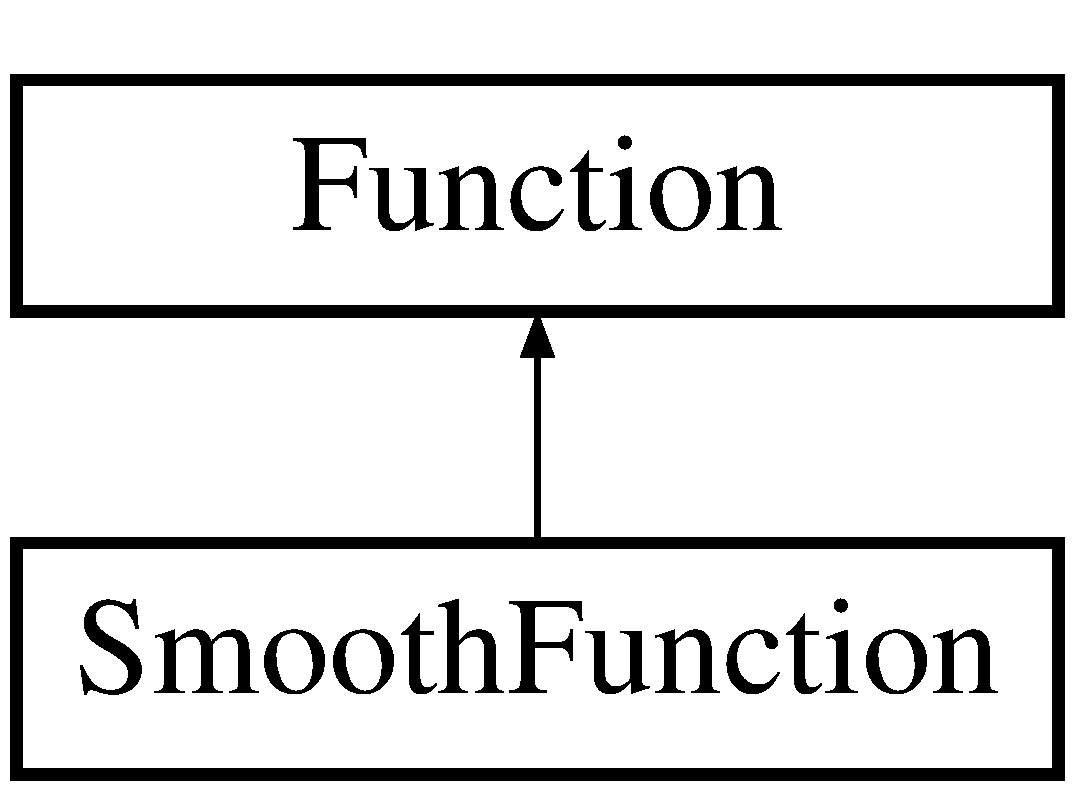
\includegraphics[height=2.000000cm]{class_smooth_function}
\end{center}
\end{figure}
\subsection*{Public Member Functions}
\begin{DoxyCompactItemize}
\item 
\hyperlink{class_smooth_function_aef997deb82c58de84cefd6559faa563b}{Smooth\+Function} (std\+::shared\+\_\+ptr$<$ \hyperlink{class_area}{Area} $>$ \+\_\+domain, std\+::shared\+\_\+ptr$<$ \hyperlink{class_function}{Function} $>$ \+\_\+grad=0)
\item 
\mbox{\Hypertarget{class_smooth_function_a0248faaf91e0e718103573574c83a517}\label{class_smooth_function_a0248faaf91e0e718103573574c83a517}} 
double \hyperlink{class_smooth_function_a0248faaf91e0e718103573574c83a517}{eval\+Grad} (const \hyperlink{classv_point}{v\+Point} \&X) const
\begin{DoxyCompactList}\small\item\em returns the evaluation of the gradient function at given point \end{DoxyCompactList}\item 
\mbox{\Hypertarget{class_smooth_function_ac71c6ad9eeb1baf639d8fc6db333033c}\label{class_smooth_function_ac71c6ad9eeb1baf639d8fc6db333033c}} 
std\+::shared\+\_\+ptr$<$ \hyperlink{class_function}{Function} $>$ \hyperlink{class_smooth_function_ac71c6ad9eeb1baf639d8fc6db333033c}{Get\+Grad} () const
\begin{DoxyCompactList}\small\item\em returns a pointer to the gradient function \end{DoxyCompactList}\end{DoxyCompactItemize}
\subsection*{Additional Inherited Members}


\subsection{Detailed Description}
\hypertarget{function_8h_DESCRIPTION}{}\subsection{D\+E\+S\+C\+R\+I\+P\+T\+I\+ON}\label{function_8h_DESCRIPTION}
The \hyperlink{class_smooth_function}{Smooth\+Function} class is derived from \hyperlink{class_function}{Function} and represents a smooth function with known gradient formula 

\subsection{Constructor \& Destructor Documentation}
\mbox{\Hypertarget{class_smooth_function_aef997deb82c58de84cefd6559faa563b}\label{class_smooth_function_aef997deb82c58de84cefd6559faa563b}} 
\index{Smooth\+Function@{Smooth\+Function}!Smooth\+Function@{Smooth\+Function}}
\index{Smooth\+Function@{Smooth\+Function}!Smooth\+Function@{Smooth\+Function}}
\subsubsection{\texorpdfstring{Smooth\+Function()}{SmoothFunction()}}
{\footnotesize\ttfamily Smooth\+Function\+::\+Smooth\+Function (\begin{DoxyParamCaption}\item[{std\+::shared\+\_\+ptr$<$ \hyperlink{class_area}{Area} $>$}]{\+\_\+domain,  }\item[{std\+::shared\+\_\+ptr$<$ \hyperlink{class_function}{Function} $>$}]{\+\_\+grad = {\ttfamily 0} }\end{DoxyParamCaption})\hspace{0.3cm}{\ttfamily [inline]}}

sets the domain and gradient function values of the smooth function 

The documentation for this class was generated from the following file\+:\begin{DoxyCompactItemize}
\item 
smooth\+\_\+function.\+h\end{DoxyCompactItemize}

\hypertarget{class_terminal_condition}{}\section{Terminal\+Condition Class Reference}
\label{class_terminal_condition}\index{Terminal\+Condition@{Terminal\+Condition}}


{\ttfamily \#include $<$terminal\+\_\+condition.\+h$>$}

Inheritance diagram for Terminal\+Condition\+:\begin{figure}[H]
\begin{center}
\leavevmode
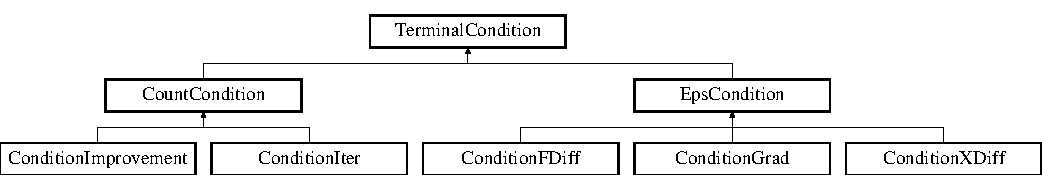
\includegraphics[height=2.333333cm]{class_terminal_condition}
\end{center}
\end{figure}
\subsection*{Public Member Functions}
\begin{DoxyCompactItemize}
\item 
\hyperlink{class_terminal_condition_a4c95c14f8dd8e7b5d6e625ff438f53d3}{Terminal\+Condition} (long \+\_\+crititer=C\+R\+I\+T\+\_\+\+I\+T\+ER)
\item 
\mbox{\Hypertarget{class_terminal_condition_a824a95f1dbd4c295cdc9eee2a1f6b464}\label{class_terminal_condition_a824a95f1dbd4c295cdc9eee2a1f6b464}} 
int \hyperlink{class_terminal_condition_a824a95f1dbd4c295cdc9eee2a1f6b464}{Get\+Crit\+Iter} () const
\begin{DoxyCompactList}\small\item\em returns critical number of iterations \end{DoxyCompactList}\item 
virtual bool \hyperlink{class_terminal_condition_ad6294bf2bd6f5e2c6164e461c24d3198}{Stop} (std\+::shared\+\_\+ptr$<$ \hyperlink{class_function}{Function} $>$ F, const std\+::vector$<$ \hyperlink{classv_point}{v\+Point} $>$ \&Approx, const std\+::vector$<$ double $>$ \&Evals) const
\item 
virtual void \hyperlink{class_terminal_condition_a55f2460a4776875211b0a4c3b449b40f}{Info} () const =0
\end{DoxyCompactItemize}
\subsection*{Friends}
\begin{DoxyCompactItemize}
\item 
std\+::ostream \& \hyperlink{class_terminal_condition_a734331dfe86aa4863287602132c3ce97}{operator$<$$<$} (std\+::ostream \&out, std\+::shared\+\_\+ptr$<$ \hyperlink{class_terminal_condition}{Terminal\+Condition} $>$ T)
\end{DoxyCompactItemize}


\subsection{Detailed Description}
\hypertarget{function_8h_DESCRIPTION}{}\subsection{D\+E\+S\+C\+R\+I\+P\+T\+I\+ON}\label{function_8h_DESCRIPTION}
The \hyperlink{class_terminal_condition}{Terminal\+Condition} class represents a method of termination of an optimization process based on the process state 

\subsection{Constructor \& Destructor Documentation}
\mbox{\Hypertarget{class_terminal_condition_a4c95c14f8dd8e7b5d6e625ff438f53d3}\label{class_terminal_condition_a4c95c14f8dd8e7b5d6e625ff438f53d3}} 
\index{Terminal\+Condition@{Terminal\+Condition}!Terminal\+Condition@{Terminal\+Condition}}
\index{Terminal\+Condition@{Terminal\+Condition}!Terminal\+Condition@{Terminal\+Condition}}
\subsubsection{\texorpdfstring{Terminal\+Condition()}{TerminalCondition()}}
{\footnotesize\ttfamily Terminal\+Condition\+::\+Terminal\+Condition (\begin{DoxyParamCaption}\item[{long}]{\+\_\+crititer = {\ttfamily CRIT\+\_\+ITER} }\end{DoxyParamCaption})}

constructor that sets the critical number of iterations to a given value 

\subsection{Member Function Documentation}
\mbox{\Hypertarget{class_terminal_condition_a55f2460a4776875211b0a4c3b449b40f}\label{class_terminal_condition_a55f2460a4776875211b0a4c3b449b40f}} 
\index{Terminal\+Condition@{Terminal\+Condition}!Info@{Info}}
\index{Info@{Info}!Terminal\+Condition@{Terminal\+Condition}}
\subsubsection{\texorpdfstring{Info()}{Info()}}
{\footnotesize\ttfamily virtual void Terminal\+Condition\+::\+Info (\begin{DoxyParamCaption}{ }\end{DoxyParamCaption}) const\hspace{0.3cm}{\ttfamily [pure virtual]}}

writes the information about the terminal condition to std\+::cout 

Implemented in \hyperlink{class_condition_grad_a76f405067bfa70754c77dfadbaad5d3e}{Condition\+Grad}, \hyperlink{class_condition_x_diff_a90e346147a31dafdf5e79809efc6babd}{Condition\+X\+Diff}, \hyperlink{class_condition_improvement_a88b5dfa7c724f8d75276d4a65eb1f398}{Condition\+Improvement}, \hyperlink{class_condition_iter_acc2c4303cd4bbc84abb9619af2f74e5c}{Condition\+Iter}, and \hyperlink{class_condition_f_diff_af632ec588748eeb234bd1df7e95f74ea}{Condition\+F\+Diff}.

\mbox{\Hypertarget{class_terminal_condition_ad6294bf2bd6f5e2c6164e461c24d3198}\label{class_terminal_condition_ad6294bf2bd6f5e2c6164e461c24d3198}} 
\index{Terminal\+Condition@{Terminal\+Condition}!Stop@{Stop}}
\index{Stop@{Stop}!Terminal\+Condition@{Terminal\+Condition}}
\subsubsection{\texorpdfstring{Stop()}{Stop()}}
{\footnotesize\ttfamily virtual bool Terminal\+Condition\+::\+Stop (\begin{DoxyParamCaption}\item[{std\+::shared\+\_\+ptr$<$ \hyperlink{class_function}{Function} $>$}]{F,  }\item[{const std\+::vector$<$ \hyperlink{classv_point}{v\+Point} $>$ \&}]{Approx,  }\item[{const std\+::vector$<$ double $>$ \&}]{Evals }\end{DoxyParamCaption}) const\hspace{0.3cm}{\ttfamily [inline]}, {\ttfamily [virtual]}}

analyzes whether the optimization process should be terminated based on the current state of the optimization 
\begin{DoxyParams}{Parameters}
{\em F} & a pointer to the function that is being optimized \\
\hline
{\em Approx} & std\+::vector of approximation vector points \\
\hline
{\em Evals} & std\+::vector of function evaluations in approximation points \\
\hline
\end{DoxyParams}
\begin{DoxyReturn}{Returns}
true if the condition requirements for termination are met and false otherwise 
\end{DoxyReturn}


Reimplemented in \hyperlink{class_condition_grad_a28d97a0d0291b24976d4499b904190a7}{Condition\+Grad}, \hyperlink{class_condition_x_diff_a375e80eb4b88db5c2823a7d4efe20972}{Condition\+X\+Diff}, \hyperlink{class_condition_improvement_a012d8db22fd6fcf8a71ab0fb5ecc1940}{Condition\+Improvement}, \hyperlink{class_condition_iter_af9de25d536e5a9af7bd711e569356533}{Condition\+Iter}, and \hyperlink{class_condition_f_diff_a31b06f62d08ab7c2ec1b011148889aab}{Condition\+F\+Diff}.



\subsection{Friends And Related Function Documentation}
\mbox{\Hypertarget{class_terminal_condition_a734331dfe86aa4863287602132c3ce97}\label{class_terminal_condition_a734331dfe86aa4863287602132c3ce97}} 
\index{Terminal\+Condition@{Terminal\+Condition}!operator$<$$<$@{operator$<$$<$}}
\index{operator$<$$<$@{operator$<$$<$}!Terminal\+Condition@{Terminal\+Condition}}
\subsubsection{\texorpdfstring{operator$<$$<$}{operator<<}}
{\footnotesize\ttfamily std\+::ostream\& operator$<$$<$ (\begin{DoxyParamCaption}\item[{std\+::ostream \&}]{out,  }\item[{std\+::shared\+\_\+ptr$<$ \hyperlink{class_terminal_condition}{Terminal\+Condition} $>$}]{T }\end{DoxyParamCaption})\hspace{0.3cm}{\ttfamily [friend]}}

overloaded output operator for std\+::cout 

The documentation for this class was generated from the following files\+:\begin{DoxyCompactItemize}
\item 
terminal\+\_\+condition.\+h\item 
terminal\+\_\+condition.\+cpp\end{DoxyCompactItemize}

\hypertarget{class_test_func01}{}\section{Test\+Func01 Class Reference}
\label{class_test_func01}\index{Test\+Func01@{Test\+Func01}}


{\ttfamily \#include $<$test\+\_\+func\+\_\+01.\+h$>$}

Inheritance diagram for Test\+Func01\+:\begin{figure}[H]
\begin{center}
\leavevmode
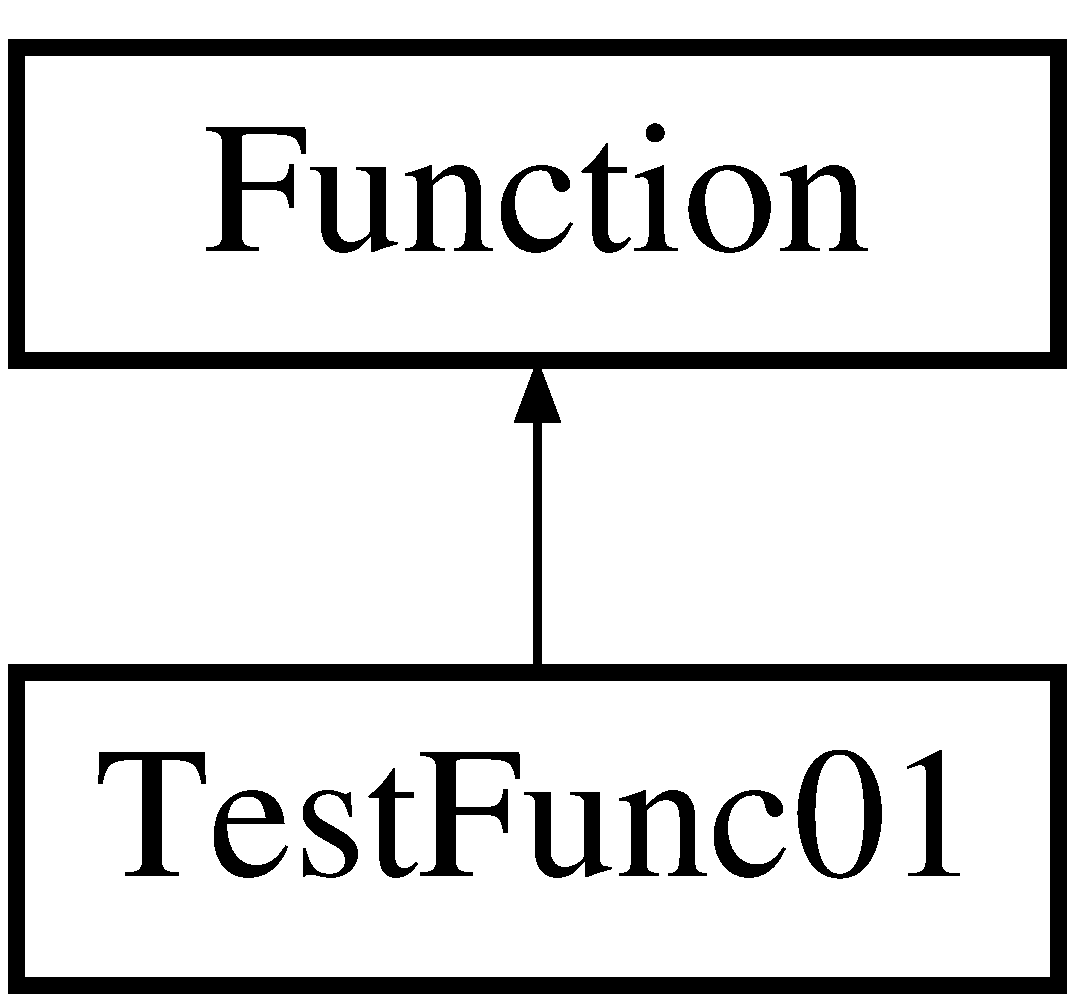
\includegraphics[height=2.000000cm]{class_test_func01}
\end{center}
\end{figure}
\subsection*{Public Member Functions}
\begin{DoxyCompactItemize}
\item 
\mbox{\Hypertarget{class_test_func01_aa0544781f37edb1d19675205c305e793}\label{class_test_func01_aa0544781f37edb1d19675205c305e793}} 
{\bfseries Test\+Func01} (std\+::shared\+\_\+ptr$<$ \hyperlink{class_area}{Area} $>$ \+\_\+domain)
\item 
virtual double \hyperlink{class_test_func01_a50b43b414345a790599ef55960a81cdb}{eval} (const \hyperlink{classv_point}{v\+Point} \&X) const
\item 
virtual void \hyperlink{class_test_func01_a731cfb0260fe58f6eab02f11449737e0}{Info} () const
\end{DoxyCompactItemize}
\subsection*{Additional Inherited Members}


\subsection{Detailed Description}
\hypertarget{function_8h_DESCRIPTION}{}\subsection{D\+E\+S\+C\+R\+I\+P\+T\+I\+ON}\label{function_8h_DESCRIPTION}
\hyperlink{class_test_func01}{Test\+Func01} is derived from \hyperlink{class_function}{Function} and represents the first test function from Khimmelblau \textquotesingle{}Nonlinear Programming\textquotesingle{} for optimization algorithms testing 

\subsection{Member Function Documentation}
\mbox{\Hypertarget{class_test_func01_a50b43b414345a790599ef55960a81cdb}\label{class_test_func01_a50b43b414345a790599ef55960a81cdb}} 
\index{Test\+Func01@{Test\+Func01}!eval@{eval}}
\index{eval@{eval}!Test\+Func01@{Test\+Func01}}
\subsubsection{\texorpdfstring{eval()}{eval()}}
{\footnotesize\ttfamily double Test\+Func01\+::eval (\begin{DoxyParamCaption}\item[{const \hyperlink{classv_point}{v\+Point} \&}]{X }\end{DoxyParamCaption}) const\hspace{0.3cm}{\ttfamily [virtual]}}

abstract method that returns the result of evaluation of the function in given point 
\begin{DoxyParams}{Parameters}
{\em X} & The point in which the function is evaluated \\
\hline
\end{DoxyParams}
\begin{DoxyReturn}{Returns}
double precision number which represents the result of the evaluation 
\end{DoxyReturn}


Implements \hyperlink{class_function_a8b9d55271a531b6f5bef09bfae0a23d9}{Function}.

\mbox{\Hypertarget{class_test_func01_a731cfb0260fe58f6eab02f11449737e0}\label{class_test_func01_a731cfb0260fe58f6eab02f11449737e0}} 
\index{Test\+Func01@{Test\+Func01}!Info@{Info}}
\index{Info@{Info}!Test\+Func01@{Test\+Func01}}
\subsubsection{\texorpdfstring{Info()}{Info()}}
{\footnotesize\ttfamily void Test\+Func01\+::\+Info (\begin{DoxyParamCaption}{ }\end{DoxyParamCaption}) const\hspace{0.3cm}{\ttfamily [virtual]}}

abstract method that prints the formula of the function 

Implements \hyperlink{class_function_a6915be18a065224ed73b1288c6125948}{Function}.



The documentation for this class was generated from the following files\+:\begin{DoxyCompactItemize}
\item 
test\+\_\+func\+\_\+01.\+h\item 
test\+\_\+func\+\_\+01.\+cpp\end{DoxyCompactItemize}

\hypertarget{class_test_func02}{}\section{Test\+Func02 Class Reference}
\label{class_test_func02}\index{Test\+Func02@{Test\+Func02}}


{\ttfamily \#include $<$test\+\_\+func\+\_\+02.\+h$>$}

Inheritance diagram for Test\+Func02\+:\begin{figure}[H]
\begin{center}
\leavevmode
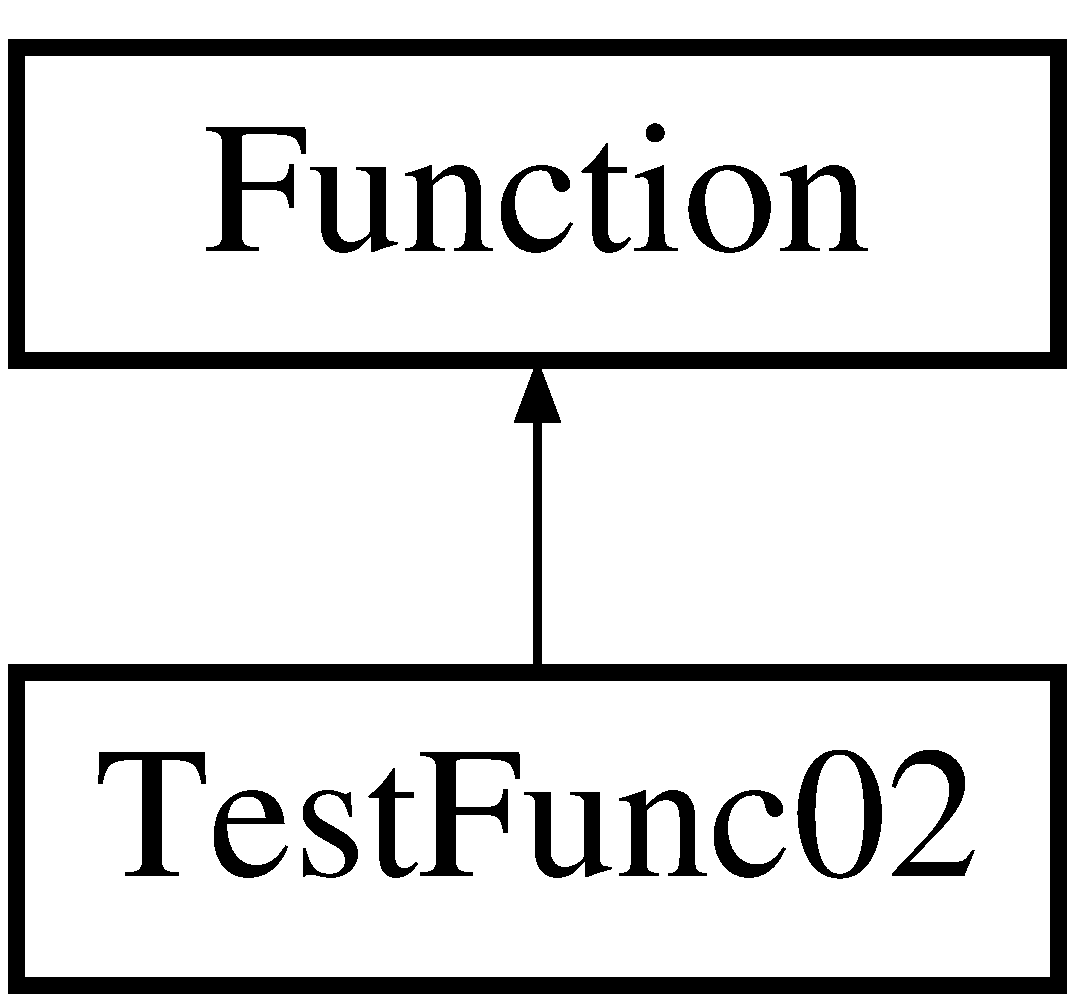
\includegraphics[height=2.000000cm]{class_test_func02}
\end{center}
\end{figure}
\subsection*{Public Member Functions}
\begin{DoxyCompactItemize}
\item 
\mbox{\Hypertarget{class_test_func02_aeb12e0d6d3c926c2074247773e44f894}\label{class_test_func02_aeb12e0d6d3c926c2074247773e44f894}} 
{\bfseries Test\+Func02} (std\+::shared\+\_\+ptr$<$ \hyperlink{class_area}{Area} $>$ \+\_\+domain)
\item 
virtual double \hyperlink{class_test_func02_af4cbebcbe8a7bd282f48ae7053c044b0}{eval} (const \hyperlink{classv_point}{v\+Point} \&X) const
\item 
virtual void \hyperlink{class_test_func02_abb39a10959e945371e662db3cd9d86ce}{Info} () const
\end{DoxyCompactItemize}
\subsection*{Additional Inherited Members}


\subsection{Detailed Description}
\hypertarget{function_8h_DESCRIPTION}{}\subsection{D\+E\+S\+C\+R\+I\+P\+T\+I\+ON}\label{function_8h_DESCRIPTION}
\hyperlink{class_test_func02}{Test\+Func02} is derived from \hyperlink{class_function}{Function} and represents the second test function from Khimmelblau \textquotesingle{}Nonlinear Programming\textquotesingle{} for optimization algorithms testing 

\subsection{Member Function Documentation}
\mbox{\Hypertarget{class_test_func02_af4cbebcbe8a7bd282f48ae7053c044b0}\label{class_test_func02_af4cbebcbe8a7bd282f48ae7053c044b0}} 
\index{Test\+Func02@{Test\+Func02}!eval@{eval}}
\index{eval@{eval}!Test\+Func02@{Test\+Func02}}
\subsubsection{\texorpdfstring{eval()}{eval()}}
{\footnotesize\ttfamily double Test\+Func02\+::eval (\begin{DoxyParamCaption}\item[{const \hyperlink{classv_point}{v\+Point} \&}]{X }\end{DoxyParamCaption}) const\hspace{0.3cm}{\ttfamily [virtual]}}

abstract method that returns the result of evaluation of the function in given point 
\begin{DoxyParams}{Parameters}
{\em X} & The point in which the function is evaluated \\
\hline
\end{DoxyParams}
\begin{DoxyReturn}{Returns}
double precision number which represents the result of the evaluation 
\end{DoxyReturn}


Implements \hyperlink{class_function_a8b9d55271a531b6f5bef09bfae0a23d9}{Function}.

\mbox{\Hypertarget{class_test_func02_abb39a10959e945371e662db3cd9d86ce}\label{class_test_func02_abb39a10959e945371e662db3cd9d86ce}} 
\index{Test\+Func02@{Test\+Func02}!Info@{Info}}
\index{Info@{Info}!Test\+Func02@{Test\+Func02}}
\subsubsection{\texorpdfstring{Info()}{Info()}}
{\footnotesize\ttfamily void Test\+Func02\+::\+Info (\begin{DoxyParamCaption}{ }\end{DoxyParamCaption}) const\hspace{0.3cm}{\ttfamily [virtual]}}

abstract method that prints the formula of the function 

Implements \hyperlink{class_function_a6915be18a065224ed73b1288c6125948}{Function}.



The documentation for this class was generated from the following files\+:\begin{DoxyCompactItemize}
\item 
test\+\_\+func\+\_\+02.\+h\item 
test\+\_\+func\+\_\+02.\+cpp\end{DoxyCompactItemize}

\hypertarget{class_test_func03}{}\section{Test\+Func03 Class Reference}
\label{class_test_func03}\index{Test\+Func03@{Test\+Func03}}


{\ttfamily \#include $<$test\+\_\+func\+\_\+03.\+h$>$}

Inheritance diagram for Test\+Func03\+:\begin{figure}[H]
\begin{center}
\leavevmode
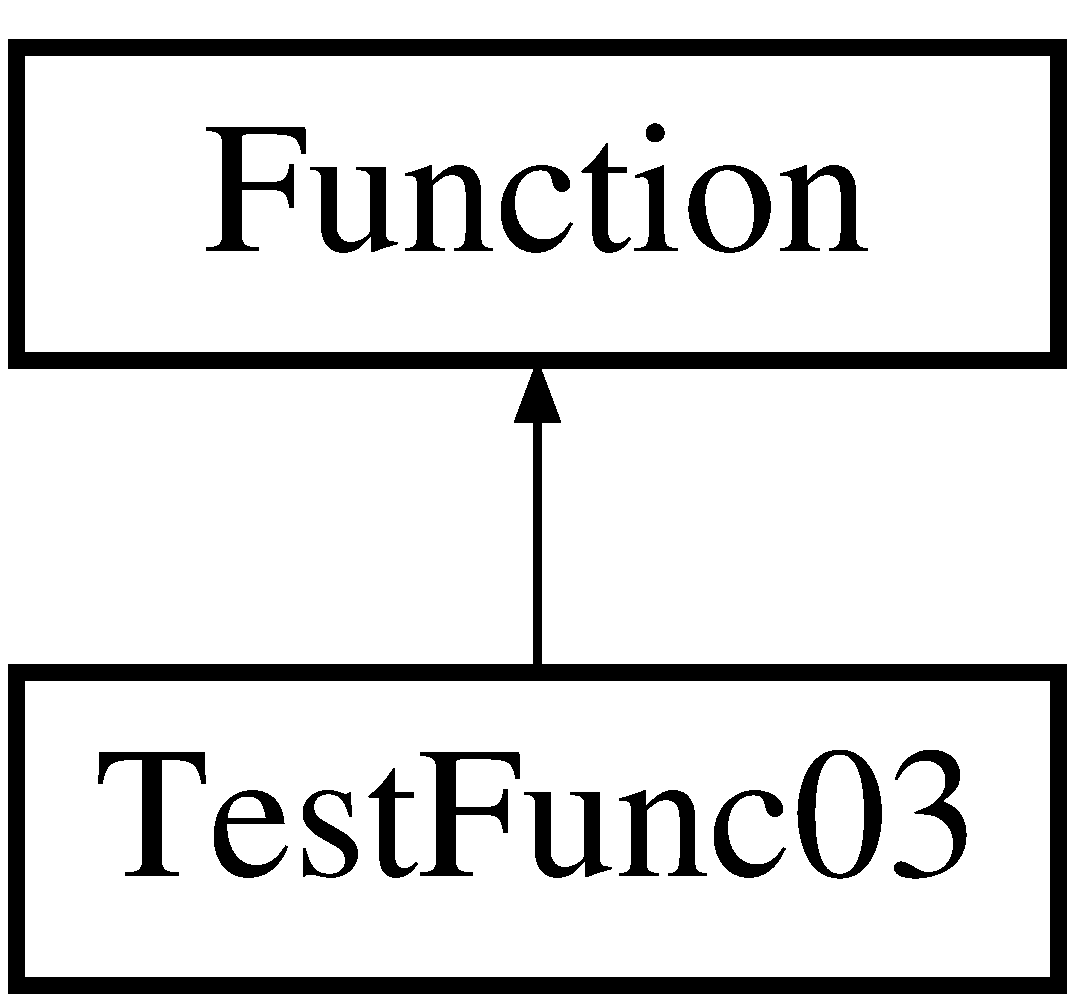
\includegraphics[height=2.000000cm]{class_test_func03}
\end{center}
\end{figure}
\subsection*{Public Member Functions}
\begin{DoxyCompactItemize}
\item 
\mbox{\Hypertarget{class_test_func03_aa3c2e1a41327b59bd09bd2bbb2663406}\label{class_test_func03_aa3c2e1a41327b59bd09bd2bbb2663406}} 
{\bfseries Test\+Func03} (std\+::shared\+\_\+ptr$<$ \hyperlink{class_area}{Area} $>$ \+\_\+domain)
\item 
virtual double \hyperlink{class_test_func03_a76417746f25346a1de704bfcac3eba47}{eval} (const \hyperlink{classv_point}{v\+Point} \&X) const
\item 
virtual void \hyperlink{class_test_func03_aab454f96f95f28f7ce1d58736d7fdf86}{Info} () const
\end{DoxyCompactItemize}
\subsection*{Additional Inherited Members}


\subsection{Detailed Description}
\hypertarget{function_8h_DESCRIPTION}{}\subsection{D\+E\+S\+C\+R\+I\+P\+T\+I\+ON}\label{function_8h_DESCRIPTION}
\hyperlink{class_test_func03}{Test\+Func03} is derived from \hyperlink{class_function}{Function} and represents the third test function from Khimmelblau \textquotesingle{}Nonlinear Programming\textquotesingle{} for optimization algorithms testing 

\subsection{Member Function Documentation}
\mbox{\Hypertarget{class_test_func03_a76417746f25346a1de704bfcac3eba47}\label{class_test_func03_a76417746f25346a1de704bfcac3eba47}} 
\index{Test\+Func03@{Test\+Func03}!eval@{eval}}
\index{eval@{eval}!Test\+Func03@{Test\+Func03}}
\subsubsection{\texorpdfstring{eval()}{eval()}}
{\footnotesize\ttfamily double Test\+Func03\+::eval (\begin{DoxyParamCaption}\item[{const \hyperlink{classv_point}{v\+Point} \&}]{X }\end{DoxyParamCaption}) const\hspace{0.3cm}{\ttfamily [virtual]}}

abstract method that returns the result of evaluation of the function in given point 
\begin{DoxyParams}{Parameters}
{\em X} & The point in which the function is evaluated \\
\hline
\end{DoxyParams}
\begin{DoxyReturn}{Returns}
double precision number which represents the result of the evaluation 
\end{DoxyReturn}


Implements \hyperlink{class_function_a8b9d55271a531b6f5bef09bfae0a23d9}{Function}.

\mbox{\Hypertarget{class_test_func03_aab454f96f95f28f7ce1d58736d7fdf86}\label{class_test_func03_aab454f96f95f28f7ce1d58736d7fdf86}} 
\index{Test\+Func03@{Test\+Func03}!Info@{Info}}
\index{Info@{Info}!Test\+Func03@{Test\+Func03}}
\subsubsection{\texorpdfstring{Info()}{Info()}}
{\footnotesize\ttfamily void Test\+Func03\+::\+Info (\begin{DoxyParamCaption}{ }\end{DoxyParamCaption}) const\hspace{0.3cm}{\ttfamily [virtual]}}

abstract method that prints the formula of the function 

Implements \hyperlink{class_function_a6915be18a065224ed73b1288c6125948}{Function}.



The documentation for this class was generated from the following files\+:\begin{DoxyCompactItemize}
\item 
test\+\_\+func\+\_\+03.\+h\item 
test\+\_\+func\+\_\+03.\+cpp\end{DoxyCompactItemize}

\hypertarget{class_test_func04}{}\section{Test\+Func04 Class Reference}
\label{class_test_func04}\index{Test\+Func04@{Test\+Func04}}


{\ttfamily \#include $<$test\+\_\+func\+\_\+04.\+h$>$}

Inheritance diagram for Test\+Func04\+:\begin{figure}[H]
\begin{center}
\leavevmode
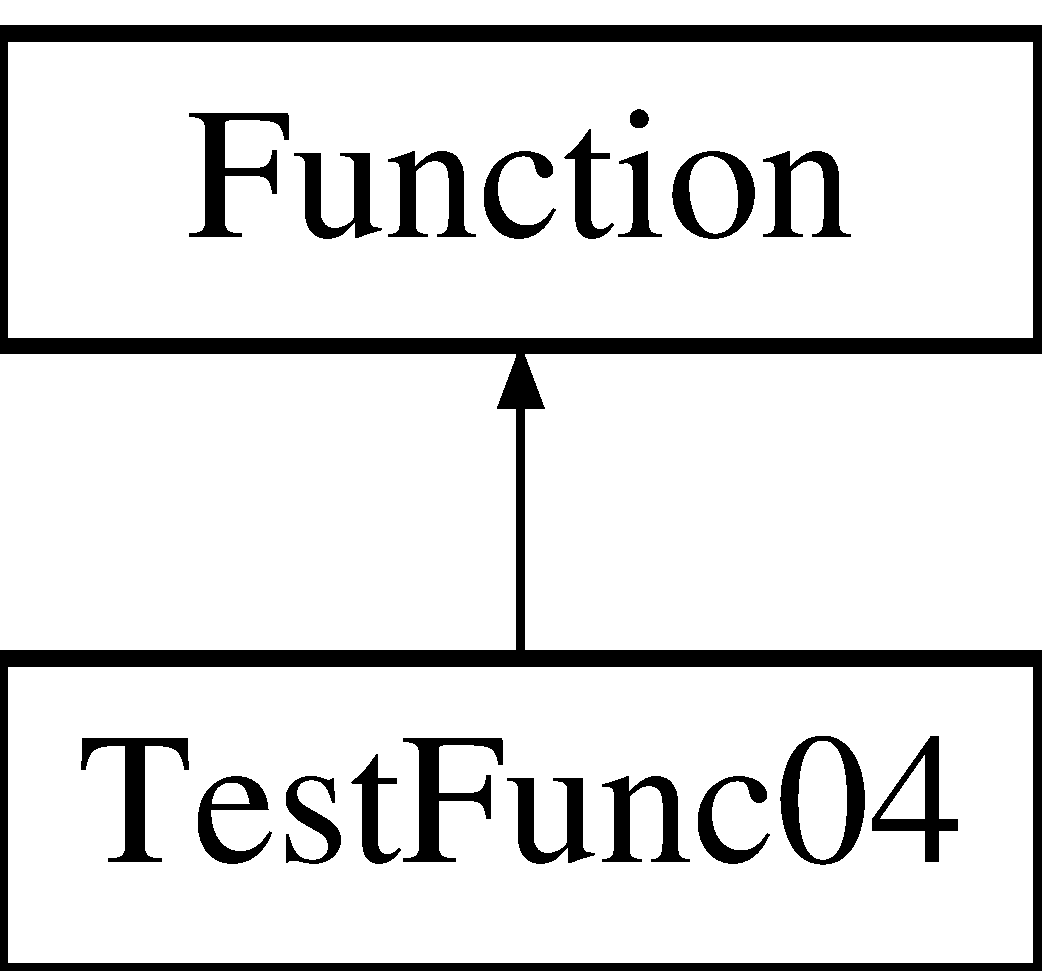
\includegraphics[height=2.000000cm]{class_test_func04}
\end{center}
\end{figure}
\subsection*{Public Member Functions}
\begin{DoxyCompactItemize}
\item 
\mbox{\Hypertarget{class_test_func04_a39b17958a522cab5a7aa4043d716cae3}\label{class_test_func04_a39b17958a522cab5a7aa4043d716cae3}} 
{\bfseries Test\+Func04} (std\+::shared\+\_\+ptr$<$ \hyperlink{class_area}{Area} $>$ \+\_\+domain)
\item 
virtual double \hyperlink{class_test_func04_a8c4666904611a414b985d17661847ec7}{eval} (const \hyperlink{classv_point}{v\+Point} \&X) const
\item 
virtual void \hyperlink{class_test_func04_a7c2bf8c334c926cbfa464081e33ac30f}{Info} () const
\end{DoxyCompactItemize}
\subsection*{Additional Inherited Members}


\subsection{Detailed Description}
\hypertarget{function_8h_DESCRIPTION}{}\subsection{D\+E\+S\+C\+R\+I\+P\+T\+I\+ON}\label{function_8h_DESCRIPTION}
\hyperlink{class_test_func04}{Test\+Func04} is derived from \hyperlink{class_function}{Function} and represents the fourth test function from Khimmelblau \textquotesingle{}Nonlinear Programming\textquotesingle{} for optimization algorithms testing 

\subsection{Member Function Documentation}
\mbox{\Hypertarget{class_test_func04_a8c4666904611a414b985d17661847ec7}\label{class_test_func04_a8c4666904611a414b985d17661847ec7}} 
\index{Test\+Func04@{Test\+Func04}!eval@{eval}}
\index{eval@{eval}!Test\+Func04@{Test\+Func04}}
\subsubsection{\texorpdfstring{eval()}{eval()}}
{\footnotesize\ttfamily double Test\+Func04\+::eval (\begin{DoxyParamCaption}\item[{const \hyperlink{classv_point}{v\+Point} \&}]{X }\end{DoxyParamCaption}) const\hspace{0.3cm}{\ttfamily [virtual]}}

abstract method that returns the result of evaluation of the function in given point 
\begin{DoxyParams}{Parameters}
{\em X} & The point in which the function is evaluated \\
\hline
\end{DoxyParams}
\begin{DoxyReturn}{Returns}
double precision number which represents the result of the evaluation 
\end{DoxyReturn}


Implements \hyperlink{class_function_a8b9d55271a531b6f5bef09bfae0a23d9}{Function}.

\mbox{\Hypertarget{class_test_func04_a7c2bf8c334c926cbfa464081e33ac30f}\label{class_test_func04_a7c2bf8c334c926cbfa464081e33ac30f}} 
\index{Test\+Func04@{Test\+Func04}!Info@{Info}}
\index{Info@{Info}!Test\+Func04@{Test\+Func04}}
\subsubsection{\texorpdfstring{Info()}{Info()}}
{\footnotesize\ttfamily void Test\+Func04\+::\+Info (\begin{DoxyParamCaption}{ }\end{DoxyParamCaption}) const\hspace{0.3cm}{\ttfamily [virtual]}}

abstract method that prints the formula of the function 

Implements \hyperlink{class_function_a6915be18a065224ed73b1288c6125948}{Function}.



The documentation for this class was generated from the following files\+:\begin{DoxyCompactItemize}
\item 
test\+\_\+func\+\_\+04.\+h\item 
test\+\_\+func\+\_\+04.\+cpp\end{DoxyCompactItemize}

\hypertarget{class_test_func05}{}\section{Test\+Func05 Class Reference}
\label{class_test_func05}\index{Test\+Func05@{Test\+Func05}}


{\ttfamily \#include $<$test\+\_\+func\+\_\+05.\+h$>$}

Inheritance diagram for Test\+Func05\+:\begin{figure}[H]
\begin{center}
\leavevmode
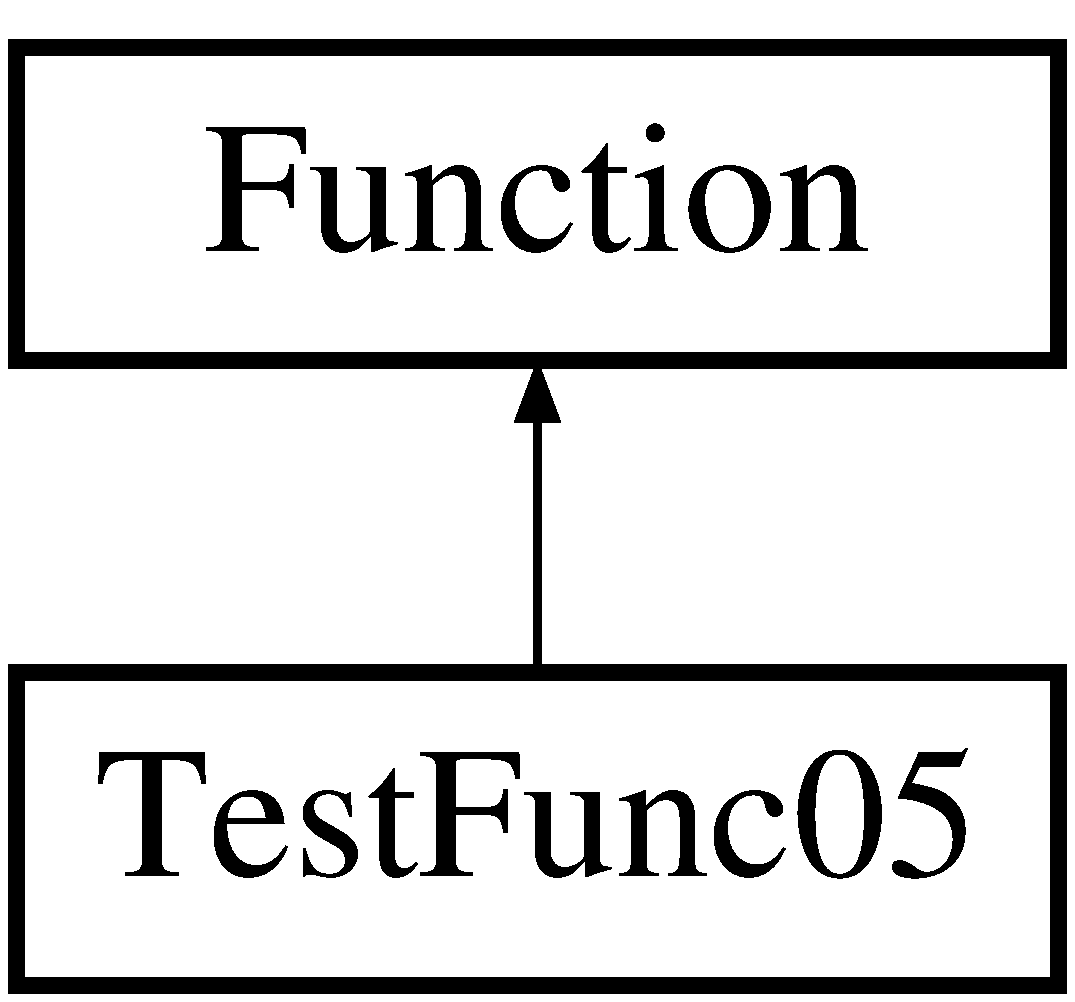
\includegraphics[height=2.000000cm]{class_test_func05}
\end{center}
\end{figure}
\subsection*{Public Member Functions}
\begin{DoxyCompactItemize}
\item 
\mbox{\Hypertarget{class_test_func05_a06502e0a2ae738dbdb79904c9264a7de}\label{class_test_func05_a06502e0a2ae738dbdb79904c9264a7de}} 
{\bfseries Test\+Func05} (std\+::shared\+\_\+ptr$<$ \hyperlink{class_area}{Area} $>$ \+\_\+domain)
\item 
virtual double \hyperlink{class_test_func05_a2848dbb9b76d0db3a701ce69ec700923}{eval} (const \hyperlink{classv_point}{v\+Point} \&X) const
\item 
virtual void \hyperlink{class_test_func05_a2a1c8696724c5195e92b4194d6205dcb}{Info} () const
\end{DoxyCompactItemize}
\subsection*{Additional Inherited Members}


\subsection{Detailed Description}
\hypertarget{function_8h_DESCRIPTION}{}\subsection{D\+E\+S\+C\+R\+I\+P\+T\+I\+ON}\label{function_8h_DESCRIPTION}
\hyperlink{class_test_func05}{Test\+Func05} is derived from \hyperlink{class_function}{Function} and represents the fifth test function from Khimmelblau \textquotesingle{}Nonlinear Programming\textquotesingle{} for optimization algorithms testing 

\subsection{Member Function Documentation}
\mbox{\Hypertarget{class_test_func05_a2848dbb9b76d0db3a701ce69ec700923}\label{class_test_func05_a2848dbb9b76d0db3a701ce69ec700923}} 
\index{Test\+Func05@{Test\+Func05}!eval@{eval}}
\index{eval@{eval}!Test\+Func05@{Test\+Func05}}
\subsubsection{\texorpdfstring{eval()}{eval()}}
{\footnotesize\ttfamily double Test\+Func05\+::eval (\begin{DoxyParamCaption}\item[{const \hyperlink{classv_point}{v\+Point} \&}]{X }\end{DoxyParamCaption}) const\hspace{0.3cm}{\ttfamily [virtual]}}

abstract method that returns the result of evaluation of the function in given point 
\begin{DoxyParams}{Parameters}
{\em X} & The point in which the function is evaluated \\
\hline
\end{DoxyParams}
\begin{DoxyReturn}{Returns}
double precision number which represents the result of the evaluation 
\end{DoxyReturn}


Implements \hyperlink{class_function_a8b9d55271a531b6f5bef09bfae0a23d9}{Function}.

\mbox{\Hypertarget{class_test_func05_a2a1c8696724c5195e92b4194d6205dcb}\label{class_test_func05_a2a1c8696724c5195e92b4194d6205dcb}} 
\index{Test\+Func05@{Test\+Func05}!Info@{Info}}
\index{Info@{Info}!Test\+Func05@{Test\+Func05}}
\subsubsection{\texorpdfstring{Info()}{Info()}}
{\footnotesize\ttfamily void Test\+Func05\+::\+Info (\begin{DoxyParamCaption}{ }\end{DoxyParamCaption}) const\hspace{0.3cm}{\ttfamily [virtual]}}

abstract method that prints the formula of the function 

Implements \hyperlink{class_function_a6915be18a065224ed73b1288c6125948}{Function}.



The documentation for this class was generated from the following files\+:\begin{DoxyCompactItemize}
\item 
test\+\_\+func\+\_\+05.\+h\item 
test\+\_\+func\+\_\+05.\+cpp\end{DoxyCompactItemize}

\hypertarget{classv_point}{}\section{v\+Point Class Reference}
\label{classv_point}\index{v\+Point@{v\+Point}}


{\ttfamily \#include $<$vpoint.\+h$>$}

\subsection*{Public Member Functions}
\begin{DoxyCompactItemize}
\item 
\hyperlink{classv_point_ab3ac707d0f2109ade8ee78a20b076e0d}{v\+Point} (std\+::vector$<$ double $>$ \+\_\+coords)
\item 
\hyperlink{classv_point_ab08b85daf7ffc356d9241cd3f62acec9}{v\+Point} (int \+\_\+dim=2)
\item 
\mbox{\Hypertarget{classv_point_aea28f9a9e8148227ef6c7e6d8066f71f}\label{classv_point_aea28f9a9e8148227ef6c7e6d8066f71f}} 
\hyperlink{classv_point_aea28f9a9e8148227ef6c7e6d8066f71f}{v\+Point} (const \hyperlink{classv_point}{v\+Point} \&other)
\begin{DoxyCompactList}\small\item\em copy constructor \end{DoxyCompactList}\item 
\mbox{\Hypertarget{classv_point_a9417173a073a0438a0edc8b742351c68}\label{classv_point_a9417173a073a0438a0edc8b742351c68}} 
\hyperlink{classv_point_a9417173a073a0438a0edc8b742351c68}{v\+Point} (\hyperlink{classv_point}{v\+Point} \&\&other)
\begin{DoxyCompactList}\small\item\em move constructor \end{DoxyCompactList}\item 
\mbox{\Hypertarget{classv_point_a6ba561bfb51c682ec29c88fb25fa70eb}\label{classv_point_a6ba561bfb51c682ec29c88fb25fa70eb}} 
virtual \hyperlink{classv_point_a6ba561bfb51c682ec29c88fb25fa70eb}{$\sim$v\+Point} ()
\begin{DoxyCompactList}\small\item\em destructor \end{DoxyCompactList}\item 
\mbox{\Hypertarget{classv_point_a9e1f704bf5ededf6933c79a927a723b4}\label{classv_point_a9e1f704bf5ededf6933c79a927a723b4}} 
int \hyperlink{classv_point_a9e1f704bf5ededf6933c79a927a723b4}{Get\+Dim} () const
\begin{DoxyCompactList}\small\item\em returns the dimeision of the vector point \end{DoxyCompactList}\item 
\mbox{\Hypertarget{classv_point_a72b0e383d2557164b7b859c70e4d2648}\label{classv_point_a72b0e383d2557164b7b859c70e4d2648}} 
double \& \hyperlink{classv_point_a72b0e383d2557164b7b859c70e4d2648}{operator\mbox{[}$\,$\mbox{]}} (int index)
\begin{DoxyCompactList}\small\item\em returns the coordinate of the vector point at given index \end{DoxyCompactList}\item 
\mbox{\Hypertarget{classv_point_a6618a9c75691efbf3c034c3f3d09697d}\label{classv_point_a6618a9c75691efbf3c034c3f3d09697d}} 
double \hyperlink{classv_point_a6618a9c75691efbf3c034c3f3d09697d}{operator\mbox{[}$\,$\mbox{]}} (int index) const
\begin{DoxyCompactList}\small\item\em returns the coordinate of the vector point at given index \end{DoxyCompactList}\item 
\mbox{\Hypertarget{classv_point_a93b3a66529a00011797a07b8084fd062}\label{classv_point_a93b3a66529a00011797a07b8084fd062}} 
\hyperlink{classv_point}{v\+Point} \& \hyperlink{classv_point_a93b3a66529a00011797a07b8084fd062}{operator=} (const \hyperlink{classv_point}{v\+Point} \&other)
\begin{DoxyCompactList}\small\item\em copy operator \end{DoxyCompactList}\item 
\mbox{\Hypertarget{classv_point_ab8419b418380071ae7b45293014991bf}\label{classv_point_ab8419b418380071ae7b45293014991bf}} 
\hyperlink{classv_point}{v\+Point} \& \hyperlink{classv_point_ab8419b418380071ae7b45293014991bf}{operator=} (const \hyperlink{classv_point}{v\+Point} \&\&other)
\begin{DoxyCompactList}\small\item\em move operator \end{DoxyCompactList}\item 
\hyperlink{classv_point}{v\+Point} \& \hyperlink{classv_point_ad0a97769619fe728547c474f856bbd66}{operator+=} (const \hyperlink{classv_point}{v\+Point} \&other)
\item 
\hyperlink{classv_point}{v\+Point} \& \hyperlink{classv_point_a3497af6c905c256e25fda5e0815bef56}{operator-\/=} (const \hyperlink{classv_point}{v\+Point} \&other)
\item 
\mbox{\Hypertarget{classv_point_a9b6165b57297692988ede20a59cd3379}\label{classv_point_a9b6165b57297692988ede20a59cd3379}} 
\hyperlink{classv_point}{v\+Point} \& \hyperlink{classv_point_a9b6165b57297692988ede20a59cd3379}{operator+=} (double offset)
\begin{DoxyCompactList}\small\item\em offsetsthe vector point by addition of the offset value to each coordinate \end{DoxyCompactList}\item 
\mbox{\Hypertarget{classv_point_a2d087a030cd39df3b548e04ea6499c7b}\label{classv_point_a2d087a030cd39df3b548e04ea6499c7b}} 
\hyperlink{classv_point}{v\+Point} \& \hyperlink{classv_point_a2d087a030cd39df3b548e04ea6499c7b}{operator-\/=} (double offset)
\begin{DoxyCompactList}\small\item\em offsetsthe vector point by subtraction of the offset value from each coordinate \end{DoxyCompactList}\item 
\mbox{\Hypertarget{classv_point_a83ce0b6a8451d2aae4af1c84cc5b8abe}\label{classv_point_a83ce0b6a8451d2aae4af1c84cc5b8abe}} 
\hyperlink{classv_point}{v\+Point} \& \hyperlink{classv_point_a83ce0b6a8451d2aae4af1c84cc5b8abe}{operator$\ast$=} (double scalar)
\begin{DoxyCompactList}\small\item\em multiplies each coordinate of the point by the scalar value \end{DoxyCompactList}\item 
\mbox{\Hypertarget{classv_point_ac0b1bd4a1f1e0472d1f21ea100c338d6}\label{classv_point_ac0b1bd4a1f1e0472d1f21ea100c338d6}} 
\hyperlink{classv_point}{v\+Point} \& \hyperlink{classv_point_ac0b1bd4a1f1e0472d1f21ea100c338d6}{operator/=} (double scalar)
\begin{DoxyCompactList}\small\item\em divides each coordinate of the point by the scalar value \end{DoxyCompactList}\end{DoxyCompactItemize}
\subsection*{Protected Attributes}
\begin{DoxyCompactItemize}
\item 
\mbox{\Hypertarget{classv_point_a01b26d19fd50e476447da555d6160bce}\label{classv_point_a01b26d19fd50e476447da555d6160bce}} 
int \hyperlink{classv_point_a01b26d19fd50e476447da555d6160bce}{dim}
\begin{DoxyCompactList}\small\item\em the dimension of the point (the number of point coordinates) \end{DoxyCompactList}\item 
\mbox{\Hypertarget{classv_point_a1bdcc85eb8914850b0c5e10aa97516de}\label{classv_point_a1bdcc85eb8914850b0c5e10aa97516de}} 
std\+::vector$<$ double $>$ \hyperlink{classv_point_a1bdcc85eb8914850b0c5e10aa97516de}{coordinates}
\begin{DoxyCompactList}\small\item\em std\+::vector of coordinates of the point \end{DoxyCompactList}\end{DoxyCompactItemize}
\subsection*{Friends}
\begin{DoxyCompactItemize}
\item 
\mbox{\Hypertarget{classv_point_a1c4599f190a262e247ba7c3593b4cfe5}\label{classv_point_a1c4599f190a262e247ba7c3593b4cfe5}} 
\hyperlink{classv_point}{v\+Point} \& \hyperlink{classv_point_a1c4599f190a262e247ba7c3593b4cfe5}{operator+} (const \hyperlink{classv_point}{v\+Point} \&left, const \hyperlink{classv_point}{v\+Point} \&right)
\begin{DoxyCompactList}\small\item\em returns the sum of two vector points \end{DoxyCompactList}\item 
\mbox{\Hypertarget{classv_point_ae0fc32c8942991e5183ee6070d749bca}\label{classv_point_ae0fc32c8942991e5183ee6070d749bca}} 
\hyperlink{classv_point}{v\+Point} \& \hyperlink{classv_point_ae0fc32c8942991e5183ee6070d749bca}{operator-\/} (const \hyperlink{classv_point}{v\+Point} \&left, const \hyperlink{classv_point}{v\+Point} \&right)
\begin{DoxyCompactList}\small\item\em subtracts one vector point from another and returns the result \end{DoxyCompactList}\item 
\hyperlink{classv_point}{v\+Point} \& \hyperlink{classv_point_ab409b6cbfb4ba84f7040ddcff0950ea3}{operator+} (const \hyperlink{classv_point}{v\+Point} \&point, double offset)
\item 
\hyperlink{classv_point}{v\+Point} \& \hyperlink{classv_point_a989b20bf1e5537591771480106d3e641}{operator-\/} (const \hyperlink{classv_point}{v\+Point} \&point, double offset)
\item 
\hyperlink{classv_point}{v\+Point} \& \hyperlink{classv_point_a3aab0a4b27ca1c92c3e690bfe7752ddd}{operator$\ast$} (const \hyperlink{classv_point}{v\+Point} \&point, double scalar)
\item 
\hyperlink{classv_point}{v\+Point} \& \hyperlink{classv_point_a71cb80dbf2851ffff4e92b87e38a3aaf}{operator/} (const \hyperlink{classv_point}{v\+Point} \&point, double scalar)
\item 
\mbox{\Hypertarget{classv_point_a5f06ca068d6617b91698fea5d816250e}\label{classv_point_a5f06ca068d6617b91698fea5d816250e}} 
std\+::ostream \& \hyperlink{classv_point_a5f06ca068d6617b91698fea5d816250e}{operator$<$$<$} (std\+::ostream \&out, const \hyperlink{classv_point}{v\+Point} \&Point)
\begin{DoxyCompactList}\small\item\em writes the information about the vector point to an std\+::ostream object \end{DoxyCompactList}\item 
\mbox{\Hypertarget{classv_point_ad65bf05cecb88ac33d7fa105e9ead1a7}\label{classv_point_ad65bf05cecb88ac33d7fa105e9ead1a7}} 
double {\bfseries norm} (const \hyperlink{classv_point}{v\+Point} \&Point)
\end{DoxyCompactItemize}


\subsection{Detailed Description}
\hypertarget{function_8h_DESCRIPTION}{}\subsection{D\+E\+S\+C\+R\+I\+P\+T\+I\+ON}\label{function_8h_DESCRIPTION}
The \hyperlink{classv_point}{v\+Point} class represents a vector point with real number coordinates 

\subsection{Constructor \& Destructor Documentation}
\mbox{\Hypertarget{classv_point_ab3ac707d0f2109ade8ee78a20b076e0d}\label{classv_point_ab3ac707d0f2109ade8ee78a20b076e0d}} 
\index{v\+Point@{v\+Point}!v\+Point@{v\+Point}}
\index{v\+Point@{v\+Point}!v\+Point@{v\+Point}}
\subsubsection{\texorpdfstring{v\+Point()}{vPoint()}\hspace{0.1cm}{\footnotesize\ttfamily [1/2]}}
{\footnotesize\ttfamily v\+Point\+::v\+Point (\begin{DoxyParamCaption}\item[{std\+::vector$<$ double $>$}]{\+\_\+coords }\end{DoxyParamCaption})}

constructor that sets the coordinates and dimension of the point based on the std\+::vector of coordinates 
\begin{DoxyParams}{Parameters}
{\em \+\_\+coords} & the coordinates of the vector \\
\hline
\end{DoxyParams}
\mbox{\Hypertarget{classv_point_ab08b85daf7ffc356d9241cd3f62acec9}\label{classv_point_ab08b85daf7ffc356d9241cd3f62acec9}} 
\index{v\+Point@{v\+Point}!v\+Point@{v\+Point}}
\index{v\+Point@{v\+Point}!v\+Point@{v\+Point}}
\subsubsection{\texorpdfstring{v\+Point()}{vPoint()}\hspace{0.1cm}{\footnotesize\ttfamily [2/2]}}
{\footnotesize\ttfamily v\+Point\+::v\+Point (\begin{DoxyParamCaption}\item[{int}]{\+\_\+dim = {\ttfamily 2} }\end{DoxyParamCaption})}

constructor that sets the dimension of the vector point and fills it with zeroes 
\begin{DoxyParams}{Parameters}
{\em \+\_\+dim} & the dimension of the point \\
\hline
\end{DoxyParams}


\subsection{Member Function Documentation}
\mbox{\Hypertarget{classv_point_ad0a97769619fe728547c474f856bbd66}\label{classv_point_ad0a97769619fe728547c474f856bbd66}} 
\index{v\+Point@{v\+Point}!operator+=@{operator+=}}
\index{operator+=@{operator+=}!v\+Point@{v\+Point}}
\subsubsection{\texorpdfstring{operator+=()}{operator+=()}}
{\footnotesize\ttfamily \hyperlink{classv_point}{v\+Point} \& v\+Point\+::operator+= (\begin{DoxyParamCaption}\item[{const \hyperlink{classv_point}{v\+Point} \&}]{other }\end{DoxyParamCaption})}

adds the coordinates of another vector point to this vector point 
\begin{DoxyParams}{Parameters}
{\em other} & vector point which is added to this vector point \\
\hline
\end{DoxyParams}
\begin{DoxyReturn}{Returns}
the resulting vector point 
\end{DoxyReturn}
\mbox{\Hypertarget{classv_point_a3497af6c905c256e25fda5e0815bef56}\label{classv_point_a3497af6c905c256e25fda5e0815bef56}} 
\index{v\+Point@{v\+Point}!operator-\/=@{operator-\/=}}
\index{operator-\/=@{operator-\/=}!v\+Point@{v\+Point}}
\subsubsection{\texorpdfstring{operator-\/=()}{operator-=()}}
{\footnotesize\ttfamily \hyperlink{classv_point}{v\+Point} \& v\+Point\+::operator-\/= (\begin{DoxyParamCaption}\item[{const \hyperlink{classv_point}{v\+Point} \&}]{other }\end{DoxyParamCaption})}

subtracts the coordinates of another vector point to this vector point 
\begin{DoxyParams}{Parameters}
{\em other} & vector point which is subtracted this vector point \\
\hline
\end{DoxyParams}
\begin{DoxyReturn}{Returns}
the resulting vector point 
\end{DoxyReturn}


\subsection{Friends And Related Function Documentation}
\mbox{\Hypertarget{classv_point_a3aab0a4b27ca1c92c3e690bfe7752ddd}\label{classv_point_a3aab0a4b27ca1c92c3e690bfe7752ddd}} 
\index{v\+Point@{v\+Point}!operator$\ast$@{operator$\ast$}}
\index{operator$\ast$@{operator$\ast$}!v\+Point@{v\+Point}}
\subsubsection{\texorpdfstring{operator$\ast$}{operator*}}
{\footnotesize\ttfamily \hyperlink{classv_point}{v\+Point}\& operator$\ast$ (\begin{DoxyParamCaption}\item[{const \hyperlink{classv_point}{v\+Point} \&}]{point,  }\item[{double}]{scalar }\end{DoxyParamCaption})\hspace{0.3cm}{\ttfamily [friend]}}


\begin{DoxyParams}{Parameters}
{\em point} & vector point coordinates of which are multiplied \\
\hline
{\em scalar} & a double by which the coordinates of the vector point are multiplied \\
\hline
\end{DoxyParams}
\begin{DoxyReturn}{Returns}
vector point with multiplied coordinates 
\end{DoxyReturn}
\mbox{\Hypertarget{classv_point_ab409b6cbfb4ba84f7040ddcff0950ea3}\label{classv_point_ab409b6cbfb4ba84f7040ddcff0950ea3}} 
\index{v\+Point@{v\+Point}!operator+@{operator+}}
\index{operator+@{operator+}!v\+Point@{v\+Point}}
\subsubsection{\texorpdfstring{operator+}{operator+}}
{\footnotesize\ttfamily \hyperlink{classv_point}{v\+Point}\& operator+ (\begin{DoxyParamCaption}\item[{const \hyperlink{classv_point}{v\+Point} \&}]{point,  }\item[{double}]{offset }\end{DoxyParamCaption})\hspace{0.3cm}{\ttfamily [friend]}}

offsets the coordinates of the point via addition of a real number to each coordinate 
\begin{DoxyParams}{Parameters}
{\em point} & the vector point that is being offset \\
\hline
{\em offset} & the double number that represents the offset value \\
\hline
\end{DoxyParams}
\begin{DoxyReturn}{Returns}
vector point with offset coordinates 
\end{DoxyReturn}
\mbox{\Hypertarget{classv_point_a989b20bf1e5537591771480106d3e641}\label{classv_point_a989b20bf1e5537591771480106d3e641}} 
\index{v\+Point@{v\+Point}!operator-\/@{operator-\/}}
\index{operator-\/@{operator-\/}!v\+Point@{v\+Point}}
\subsubsection{\texorpdfstring{operator-\/}{operator-}}
{\footnotesize\ttfamily \hyperlink{classv_point}{v\+Point}\& operator-\/ (\begin{DoxyParamCaption}\item[{const \hyperlink{classv_point}{v\+Point} \&}]{point,  }\item[{double}]{offset }\end{DoxyParamCaption})\hspace{0.3cm}{\ttfamily [friend]}}

offsets the coordinates of the point via subtraction of a real number to each coordinate 
\begin{DoxyParams}{Parameters}
{\em point} & the vector point that is being offset \\
\hline
{\em offset} & the double number that represents the offset value \\
\hline
\end{DoxyParams}
\begin{DoxyReturn}{Returns}
vector point with offset coordinates 
\end{DoxyReturn}
\mbox{\Hypertarget{classv_point_a71cb80dbf2851ffff4e92b87e38a3aaf}\label{classv_point_a71cb80dbf2851ffff4e92b87e38a3aaf}} 
\index{v\+Point@{v\+Point}!operator/@{operator/}}
\index{operator/@{operator/}!v\+Point@{v\+Point}}
\subsubsection{\texorpdfstring{operator/}{operator/}}
{\footnotesize\ttfamily \hyperlink{classv_point}{v\+Point}\& operator/ (\begin{DoxyParamCaption}\item[{const \hyperlink{classv_point}{v\+Point} \&}]{point,  }\item[{double}]{scalar }\end{DoxyParamCaption})\hspace{0.3cm}{\ttfamily [friend]}}


\begin{DoxyParams}{Parameters}
{\em point} & vector point coordinates of which are divided \\
\hline
{\em scalar} & a double by which the coordinates of the vector point are divided \\
\hline
\end{DoxyParams}
\begin{DoxyReturn}{Returns}
vector point with divided coordinates 
\end{DoxyReturn}


The documentation for this class was generated from the following files\+:\begin{DoxyCompactItemize}
\item 
vpoint.\+h\item 
vpoint.\+cpp\end{DoxyCompactItemize}

\chapter{File Documentation}
\hypertarget{function_8h}{}\section{function.\+h File Reference}
\label{function_8h}\index{function.\+h@{function.\+h}}
{\ttfamily \#include $<$memory$>$}\newline
{\ttfamily \#include $<$string$>$}\newline
{\ttfamily \#include \char`\"{}vpoint.\+h\char`\"{}}\newline
{\ttfamily \#include \char`\"{}area.\+h\char`\"{}}\newline
\subsection*{Classes}
\begin{DoxyCompactItemize}
\item 
class \hyperlink{class_function}{Function}
\end{DoxyCompactItemize}


\subsection{Detailed Description}
\begin{DoxyAuthor}{Author}
Nikita Fyodorov 
\end{DoxyAuthor}
\begin{DoxyVersion}{Version}
1.\+0
\end{DoxyVersion}
\hypertarget{function_8h_DESCRIPTION}{}\subsection{D\+E\+S\+C\+R\+I\+P\+T\+I\+ON}\label{function_8h_DESCRIPTION}
The \hyperlink{class_function}{Function} class represents an abstract vector-\/function which can be evaluated in given domain 
%--- End generated contents ---

% Index
\backmatter
\newpage
\phantomsection
\clearemptydoublepage
\addcontentsline{toc}{chapter}{Index}
\printindex

\end{document}
